\documentclass[a4paper,twoside,openright,fleqn,11pt]{book}
\usepackage[T1]{fontenc}
\usepackage[light,slantedGreeks]{kpfonts}
\usepackage[utf8]{inputenc}
\usepackage[italian]{babel}

%%%%% Pacchetti caricati
\usepackage{microtype}
\usepackage{layaureo}
\usepackage[autostyle=true]{csquotes}
\usepackage[style=authoryear,hyperref,abbreviate=false,backend=bibtex]{biblatex}
\usepackage{fancyhdr,emptypage}
\usepackage{tensor} % per rappresentare i tensori
\usepackage[font=small,format=hang,labelfont=bf,textformat=period]{caption}
% per tabelle e figure
\usepackage{booktabs,longtable,graphicx,sidecap,subfig}
\usepackage{tikz}
% `mathtools' serve per definire la norma e il valore assoluto
\usepackage{mathtools}
% pacchetti matematici dell'American Mathematical Society
\usepackage{amsthm}
% `bm' serve per scrivere i vettori in corsivo con il comando
% `\bm{vettore}'. Deve sostituire il comando `\mathbf{vettore}' perché questo
% restituisce erroneamente lettere in tondo, non in corsivo e non funziona con
% le lettere greche.
\usepackage{bm}
\usepackage{makeidx}
\usepackage{siunitx}
\usepackage{hyperref}
%%%%% Fine pacchetti

%%%%% Impostazioni
%% testatine.
\pagestyle{fancy}
\fancyhf{} % svuota tutti i campi delle testatine e dei piedi
\setlength{\headheight}{14pt}
% Nella testatina (`head') a destra (`R') nelle pagine pari (`E') mettiamo il
% nome del capitolo (`\leftmark'), non tutto maiuscolo (`\nouppercase'). Sulla
% sinistra (`L') delle pagine dispari (`O') mettiamo il nome del paragrafo
% (`\rightmark').
\fancyhead[RE]{\slshape\footnotesize\nouppercase{\leftmark}}
\fancyhead[LO]{\slshape\footnotesize\nouppercase{\rightmark}}
% All'esterno di ogni pagina (cioè a sinistra (`L') nelle pagine pari (`E') e a
% destra (`R') nelle pagine dispari (`O')), nella testatina (`head') mettiamo il
% numero della pagina (`\thepage').
\fancyhead[LE,RO]{\thepage}

% impostazioni per il pacchetto `hyperref'. Per l'elenco di tutte le opzioni del
% documento consulta il manuale: `texdoc hyperref'
\hypersetup{
  pdftitle={Cosmologia},
  pdfauthor={Mosè Giordano},
  breaklinks=true,% permette di spezzare i link su più righe
  bookmarksnumbered,% inserisce i numeri delle sezioni nei segnalibri
  hidelinks % link neri e senza bordi colorati, adatto per la stampa
}

\sisetup{per-mode=symbol,
  inter-unit-product=\ensuremath{{}\cdot{}},
  exponent-product=\cdot,
  output-product=\cdot,
  separate-uncertainty=true,
  math-micro=\muup,
  text-micro=\ensuremath{\muup},
}

% Posiziona le didascalie sopra le tabelle
\captionsetup[table]{position=top}

\addbibresource{bibliografia.bib} % nome del file contenente la bibliografia
\defbibheading{bibliography}[\refname]{\chapter*{#1}\markboth{#1}{#1}}

\theoremstyle{plain}
\newtheorem*{teorema}{Teorema}

% librerie ti TikZ
\usetikzlibrary{calc,decorations.pathmorphing,decorations.pathreplacing,
  intersections,matrix,backgrounds}
%%%%% Fine impostazioni

%%%%% Comandi personalizzati
% ridefinisco i comandi per alcune lettere greche in modo che si usino le
% varianti
\renewcommand{\phi}{\varphi}
\renewcommand{\epsilon}{\varepsilon}

% Comando per indicare la variazione di una quantità.  Deve produrre una delta
% maiuscola diritta, visto che carico il pacchetto `kpfonts' con l'opzione
% `slantedGreeks' uso la macro `\Deltaup'.
\newcommand{\var}{\Deltaup}

% comando per evidenziare le sezioni da completare o espandere.  NOTA: è un
% comando provvisorio, serve solo durante la scrittura del testo, ricordarsi di
% eliminarlo quando non serve più.
\newcommand{\completare}[1]{\textcolor{red}{#1 (COMPLETARE)}}

% Operatori
\newcommand*{\dd}{\mathop{}\!\mathrm{d}} % Operatore differenziale \dd
\newcommand*{\cdd}{\mathop{}\!\mathrm{D}} % Differenziale covariante \cdd
\DeclareMathOperator{\e}{\mathrm{e}} % Numero di Eulero
\DeclareMathOperator{\diag}{diag}
\DeclareMathOperator{\uimm}{\mathrm{i}} % unità immaginaria
\DeclareMathOperator{\arcsinh}{arcsinh}
% Operatore valore assoluto \abs{x}. Usa \abs*{} per le frazioni
\DeclarePairedDelimiter{\abs}{\lvert}{\rvert}
% Operatore norma \norm{x}. Usa \norm*{} per le frazioni
\DeclarePairedDelimiter{\norm}{\lVert}{\rVert}

%% Derivate
% Derivata totale: \toder[ordine]{funzione}{variabile}
\newcommand*{\toder}[3][]{\frac{{\dd^{#1}}#2}{\dd {#3}^{#1}}}
% Derivata covariante: \covder[ordine]{tensore}{variabile}
\newcommand*{\covder}[3][]{\frac{{\cdd^{#1}}#2}{\dd {#3}^{#1}}}
% Derivata lungo una curva: \covder[ordine]{tensore}
\newcommand*{\curder}[2][]{\frac{{\cdd^{#1}}#2}{\cdd \tau^{#1}}}
% operatore d'alambertiano.  Definisco un comando specifico nel caso in cui si
% decidesse di cambiare la notazione (per esempio \Box invece di \Box^{2}).
\newcommand{\dalamb}{\Box^{2}}

% Derivata parziale \parder[ordine]{funzione}{variabile}
% Per la definizione del comando `parder' (per inserire le derivate parziali)
% vedi
% http://www.guitex.org/home/index.php?option=com_kunena&func=view&catid=5&id=42178&Itemid=60#42199
\makeatletter
\newcommand{\parder}[2]{\begingroup
  \@tempswafalse\toks@={}\count@=\z@
  \@for\next:=#2\do
    {\expandafter\check@var\next\@nil
     \advance\count@\parder@exp
     \if@tempswa
       \toks@=\expandafter{\the\toks@\,}%
     \else
       \@tempswatrue
     \fi
     \toks@=\expandafter{\the\expandafter\toks@\expandafter\partial\parder@var}}%
  \frac{\partial\ifnum\count@=\@ne\else^{\number\count@}\fi#1}{\the\toks@}%
  \endgroup}
\def\check@var{\@ifstar{\mult@var}{\one@var}}
\def\mult@var#1#2\@nil{\def\parder@var{#2^{#1}}\def\parder@exp{#1}}
\def\one@var#1\@nil{\def\parder@var{#1}\chardef\parder@exp\@ne}
\makeatother

% Derivate per le formule in linea (usare \frac in linea è eccessivo). La `l'
% iniziale nel nome distingue questi comandi da quelli per le formule fuori
% corpo. Non uso `\dd' ma `\mathrm{d}' perché nelle formule in linea `\dd'
% aggiunge una spaziatura non adatta. Non sono dei comandi bellissimi, ma
% permettono di passare facilmente da formula in linea a fuori corpo e viceversa
% cambiando una lettera.
% Derivata totale: \ltoder[ordine]{funzione}{variabile}
\newcommand*{\ltoder}[3][]{\mathrm{d}^{#1}#2 / \mathrm{d} {#3}^{#1}}
% Derivata parziale: \lparder[ordine]{funzione}{variabile}
\newcommand*{\lparder}[3][]{\partial^{#1} #2 / \partial {#3}^{#1}}
% NOTA: `\parder' e `\lparder' non sono completamente interscambiabili, il primo
% comando è molto più complesso e permette di inserire le derivate miste, a
% differenza del secondo.

% Versore. Esempi: versore x: `\versore{x}', versore i: \versor{\imath}, versore
% j: \versor{\jmath} (solo `i' e `j' richiedono `\imath' e `\jmath', altrimenti
% il puntino litiga con `\hat')
\newcommand*{\versor}[1]{\hat{\bm{#1}}}

%% Campi notevoli
\let\numberset\mathbb
\newcommand{\N}{\numberset{N}}	% Naturali \N
\newcommand{\Z}{\numberset{Z}}	% Interi \Z
\newcommand{\R}{\numberset{R}}	% Reali \R
\newcommand{\C}{\numberset{C}}	% Complessi \C
\newcommand{\M}{\numberset{M}}	% spazio-tempo di Minkowski

% unità di misura aggiuntive (non-SI)
\DeclareSIUnit\dyne{dyn} % dyne
\DeclareSIUnit\erg{erg} % erg
\DeclareSIUnit\tonne{t} % tonnellata ("tonne" in inglese)
\DeclareSIUnit\parsec{pc} % parsec
\DeclareSIUnit\lightyear{ly} % anno luce
\DeclareSIUnit\radian{rad} % radiante
\DeclareSIUnit\solarmass{\ensuremath{M_{\odot}}} % massa solare
%%%%% Fine comandi personalizzati
\makeindex{}

\begin{document}

\frontmatter{}

%% copertina, rielaborazione dell'esempio `\titleGP' di pagina 34 del file di
%% documentazione `titlepages.pdf'
\thispagestyle{empty}
\begingroup
\scshape
\centering
\vspace*{\baselineskip}
\rule{\textwidth}{1.6pt}\vspace*{-\baselineskip}\vspace*{2pt}
\rule{\textwidth}{0.4pt}\\[0.2\baselineskip]
{\Huge Cosmologia}\\[0.2\baselineskip]
\rule{\textwidth}{0.4pt}\vspace*{-\baselineskip}\vspace{3.2pt}
\rule{\textwidth}{1.6pt}\\[\baselineskip]
\vspace*{2\baselineskip}
{\Large
  Mosè Giordano e  Gabriele Ingrosso} \\
{\it Dipartimento di Matematica e Fisica \\
 Università del Salento, Lecce}

\vfill

\includegraphics[width=2cm]{figure/logo_unisalento}\\
\today\par
\endgroup
%% Fine copertina

\newpage
{\large
 Appunti del corso di Gravitazione e Cosmologia, Laurea Magistrale in Fisica,
 tenuto dal Prof. Gabriele Ingrosso nell'anno accademico 2011-2012.

 Il lavoro è \emph{in progress} per cui sono gradite segnalazioni di errori ed
 in generale commenti che migliorino il testo.}

\cleardoublepage{}
\tableofcontents{} % indice generale
\cleardoublepage{}
\listoffigures{} % elenco delle figure

\cleardoublepage{}
\mainmatter{}
\chapter{Cosmografia}
\label{cha:cosmografia}

\section[Introduzione]{Introduzione\footnote{In questo paragrafo introduttivo
    alla Cosmologia ho seguito gli appunti del corso di Cosmologia di
    A. Cavaliere, Università di Roma.}}

L'inizio della Cosmologia moderna può essere datato agli anni '20 del secolo
scorso con la scoperta di stelle variabili periodiche del tipo delle Cefeidi in
alcune nebulose a spirale tra cui M31 nella costellazione di Andromeda.  Poiché
era nota per le Cefeidi una relazione empirica tra periodo $P$ e luminosità
assoluta $L$, la distanza $D$ di M31 è determinata attraverso la misura del
flusso $F$ e l'utilizzo della relazione (valida nel caso euclideo)
\begin{equation}
  D=\left( \frac{L}{4 \pi F} \right)^{1/2}
\end{equation}
La distanza di M31 risultò\footnote{Tale distanza risultò in seguito errata per
  difetto a causa di una sottostima di $L$ --- dovuta all'aver trascurato
  l'assorbimento della luce da parte del mezzo interstellare (ISM).  Oggi noi
  sappiamo che la distanza di M31 è 770 kpc.} di circa 240 kpc (1 pc equivale a
$3.08 \times 10^{18}$ cm $\equiv 3.3$ anni luce) e pertanto molto maggiore delle
dimensioni visibili della nostra galassia (la Galassia o Via Lattea) che allora
erano stimate in 10 kpc, dimostrando in modo conclusivo che M31 costituiva un
intero sistema di stelle esterno alla Galassia.

La scoperta, comunicata da E. Hubble il 1 gennaio 1925, pose fine a una lunga
controversia tra gli astronomi sulla natura delle nebulose che furono
interpretate definitivamente come sistemi di stelle (universi isola) analoghi
alla Galassia.

È da sottolineare subito che le osservazioni astronomiche hanno la seguente
peculiarità.  A causa della velocità finita di propagazione della luce, quando
noi guardiamo lontano nello spazio, necessariamente guardiamo indietro nel tempo
e alla distanza $D$ corrisponde il tempo nel passato
\begin{equation}
  \Delta T = \frac{D}{c}
\end{equation}
per cui noi vediamo M31, la più vicina tra le grandi galassie a spirale simili
alla Galassia, come era 2.5 milioni di anni fa.

Noi viviamo in una Galassia a spirale tipica, di cui il Sole è una stella media
tra le circa $\simeq 3 \times 10^{11}$ che la compongono.  La luminosità
complessiva della Galassia è $L_G \simeq 2 \times 10^{10} L_{\odot}$ (la
luminosit solare è $L_{\odot} = 3.90 \times 10^{33}$ erg s$^{-1}$), mentre la
massa della Galassia è $M_G \simeq 10^{11} M_{\odot}$.

La densità media della Galassia, considerando gli atomi componenti le stelle e
una modesta quantità di gas interstellare uniformemente diffusi all'interno
della Galassia, è $\rho_G \simeq 10^{-23}$ g cm$^{-3}$, corrispondente a circa 5
atomi di idrogeno al cm$^{3}$.  È questa una densità estremamente bassa se
confrontata, ad esempio, con quella dell'aria.  Tuttavia, a causa delle enormi
dimensioni, essa è sufficiente a fare della Galassia un sistema isolato
auto-gravitante in cui le forze gravitazionali interne sono in equilibrio con i
moti delle stelle.

La Galassia è circondata in ogni sua parte, in media uniformemente, da altre
``isole di stelle'' (galassie) e la separazione media delle galassie è circa 3
Mpc.

In realtà vi è una netta tendenza delle galassie a formare gruppi, a loro volta
autogravitanti, di varia consistenza: da sistemi binari, a gruppi di poche
decine di galassie\footnote{La Galassia fa parte del Gruppo Locale costituito da
  25 galassie, delle quali M31 è la più grande e la Galassia è seconda per
  dimensioni.} fino agli ammassi composti da migliaia di galassie come, ad
esempio, Coma e Virgo, a distanza di circa 20 Mpc.

In sostanza, la materia tende a condensarsi su scale di dimensioni crescenti:
\begin{itemize}
\item il gas $\to$ stelle (di dimensioni $R_{\odot} \simeq 10^6$ km)
\item le stelle $\to$ galassie (di dimensioni fino a $R_G \simeq$ 100 kpc)
\item le galassie $\to$ gruppi o ammassi (di dimensioni fino a $R_{Cl}\simeq 3-10$ Mpc)
\item gli ammassi $\to$ super-ammassi (di dimensioni $\simeq$ 50 Mpc)
\end{itemize}
Questi ultimi non sono sistemi in equilibrio gravitazionale ben isolati e
appaiono prevalentemente contigui.  Le condensazioni di dimensioni
progressivamente maggiori hanno densità via via minori, mentre aumenta
fortemente il fattore di riempimento, cioè il rapporto tra il volume occupato
dai componenti ed il volume totale del sistema: le stelle riempiono solo una
frazione minuscola del volume delle galassie (la distanza media tra le stelle è
circa 1 pc) mentre i super-ammassi sono contigui.

La gerarchia di condensazioni termina con i super-ammassi e a dimensioni
superiori a 100 Mpc non si osservano strutture ben definite.  I radio telescopi
permettono di osservare a distanze maggiori dei telescopi ottici ed essi
rivelano sorgenti radio di cui alcune sono connesse con le galassie ancora
visibili otticamente mentre altre sono più lontane; la distribuzione di queste
radio sorgenti non presenta differenze nelle varie direzioni nel cielo.

{In conclusione su scale di 100 Mpc l'Universo appare isotropo ed omogeneo, cioè
  con le stesse proprietà in ogni direzione ed in ogni luogo: esso gode quindi
  di simmetria spaziale massima (\emph{Principio Cosmologico}).}

Ha senso quindi parlare di densità media dell'Universo considerando la materia
visibile nelle stelle come diffusa uniformemente.  Ne risulta una densità media
$\rho_*(t_0) \simeq 10^{-31}$ gr cm$^{-3}$ (2 atomi di idrogeno in 10 m$^3$).

Quando si arriva a scale dell'ordine dei Gpc ha senso chiedersi se le proprietà
geometriche dello spazio siano ancora di tipo "Euclideo" o meno; per esempio,
con riferimento alle superfici 2-dimensionali, ci si può chiedere se la somma
degli angoli interni di un triangolo sia $180^{\circ}$ o maggiore, come per
superfici con curvatura positiva, o minore, come per superfici di curvatura
negativa, o se una sfera con distanza radiale $D$ abbia superficie $4 \pi D^2$ e
così via.

La risposta alla domanda sulla possibile geometria dell'Universo è fornita dalla
Teoria della Relatività Generale applicata alla Cosmologia.  Nei modelli
cosmologici più semplici (modelli di Friedmann senza costante cosmologica) si
distinguono tre possibili tipi di geometria: oltre al caso euclideo, sono
possibili spazi a curvatura positiva e a curvatura negativa.  I tre casi sono
indicati con $k=0,+1,-1$ e queste tre possibilità sono ricondotte a misure
fisiche della densità media dell'Universo all'istante attuale
$\rho_0=\rho(t_0)$.  Risulterà infatti definita una densità critica $\rho_c
\simeq 1.1 \times 10^{-29}$ gr cm$^{-3}$ (5 atomi di idrogeno per m$^3$, da
confrontare con i 0.2 atomi di idrogeno per m$^3$ cui ammonta la densità media
di materia visivile), per cui:
\begin{itemize}
\item se $\rho_0 < \rho_c \implies k=-1$, curvatura spaziale è negativa
  (universo aperto);
\item se $\rho_0 = \rho_c \implies k=0$ , curvatura spaziale è nulla;
\item se $\rho_0 > \rho_c \implies k=+1$, curvatura spaziale è positiva
  (universo chiuso).
\end{itemize}
La questione delle possibili 3-geometrie dell'Universo può essere affrontata
anche dal punto di vista geometrico con misure di distanza (magnitudine
apparente $m$) e red-shift $z$ (velocità di espansione) su grande scala.  Questo
però comporta la necessità di definire una classe di oggetti (indicatori di
distanza) la cui luminosità non varia con la distanza (indietro nel tempo).  Si
costruiscono così alcuni diagrammi osservativi $m-z$, noti anche come diagrammi
di Hubble, la cui analisi conduce alla stima di importanti parametri
cosmologici.  In particolare, poichè risulterà $\rho_0 = \rho_c$ avremo la
necessità di ipotizzare la presenza di Dark Matter (DM) (materia oscura, non
visibile) che d'altra parte non potrà essere totalmente in forma barionica
poichè la teoria della Nucleosintesi degli elementi leggeri (con $A \le 4$)
sviluppata da Gamov negli anni '40 pone un limite superiore ad $\Omega_B \equiv
\rho_{B}(t_0) / \rho_c < 0.05$.

Dopo il 1924 cominciò a porsi nella comunità astronomica la domanda se
l'Universo fosse statico, cioè se le distanze tra le galassie rimanessero
costanti nel tempo.  Fu ancora~\textcite{1929PNAS...15..168H} a suggerire una
risposta negativa a questa domanda verificando con centinaia di osservazioni che
le galassie si allontanano l'una dall'altra con una velocità $v_H$ proporzionale
alla distanza
\begin{equation}
  v_H  = H_0 D.
\end{equation}
Tale relazione (valida per distanze $D$ non troppo grandi) è nota come
\emph{legge di Hubble}.  In essa la costante $H_0$ (le cui dimensioni sono
l'inverso di un tempo) fu ricalibrata più volte dai tempi di Hubble e il valore
oggi accettato è $H_0 \simeq 65$ km s$^{-1}$ Mpc$^{-1}$. {Entro la precisione
  delle misure, $H_0$ è uguale in tutte le direzioni, il che costituisce una
  ulteriore manifestazione dell'isotropia dell'Universo}.

La legge di Hubble dice che l'Universo è soggetto ad una evoluzione cinematica
nel senso dell'espansione: mentre le dimensioni dei sistemi auto-gravitanti
(come le galassie e gli ammassi) rimangono costanti, le loro distanze reciproche
aumentano nel tempo, e ad ogni tempo esse sono sempre la stessa frazione della
"scala dell'Universo $R(t)$.

L'unità di misura più conveniente per la scala attuale $R_0$ dell'Universo è la
distanza $c/H_0 \simeq 14$ miliardi di anni luce, la distanza alla quale la
legge di Hubble darebbe $v=c$.  Questa distanza è detta \emph{raggio di Hubble}
o \emph{orizzonte di Hubble}.  La legge di Hubble dice anche che se la velocità
con cui le galassie si allontano fosse rimasta costante, a un tempo del passato
pari a $1/H_0 \simeq 14$ miliardi di anni le galassie sarebbero state così
vicine fino a toccarsi.  Questo istante di tempo (detto \emph{tempo di Hubble})
fornisce un limite superiore all'età dell'Universo.  Infatti poichè è intuitivo
che il moto delle galassie sia via via decelerato dalla gravità ($\ddot{R} <
0$), nel passato la velocità di recessione delle galassie era maggiore e quindi
il tempo di Hubble (che è ottenuto assumendo che $R(t) = \dot{R}_0 t$) è un
limite superiore all'età dell'Universo.

Il 1965 è la terza data fondamentale della Cosmologia (dopo il 1924 e il 1929)
perchè in quell'anno la scoperta della radiazione di fondo cosmico (CMB)
dimostrò che l'Universo è soggetto ad una evoluzione fisica.
\textcite{1965ApJ...142..419P} notarono in un ricevitore a microonde costruito
per altri scopi un rumore di fondo debole ma costante nel tempo e in tutte le
direzioni.

Da allora, numerose misure (con palloni e satelliti poiché l'atmosfera non è
trasparente alla radiazione nella banda delle microonde) hanno dimostrato che la
radiazione di fondo cosmico:
\begin{itemize}
\item ha una distribuzione spettrale di corpo nero a una temperatura $T \simeq
  2.7$K, cioè presenta lo spettro tipico della radiazione elettromagnetica in
  equilibrio con la materia alla stessa temperatura;
\item è strettamente isotropa in tutte le direzioni fino a livelli $\Delta T/T
  \simeq 10^{-5}$.  Comunque, bisogna prima sottrarre una anisotropia detta di
  dipolo, che contribuisce con $\Delta T/T \simeq 10^{-3}$, dovuta al moto della
  Terra (somma vettoriale delle velocità della Terra rispetto al Sole, del
  sistema solare rispetto al centro della Galassia, della Galassia rispetto al
  Gruppo Locale e di questo rispetto al Super Ammasso Locale) rispetto alla
  ``superficie di ultimo scattering''.
\end{itemize}
Lo spettro della CMB è di corpo nero, cioè quello tipico della radiazione in
equilibrio con la materia.  Ma oggi la densità media dell'Universo (0.2 atomi di
idrogeno per m$^3$) è così piccola da non permettere ai fotoni di portarsi in
equilibrio con la materia.  Possiamo stimare il tempo $T_0$ che intercorre tra
due successive collisioni di uno stesso fotone con gli atomi di idrogeno, la cui
densità sia $n_H(t_0)$, attraverso la relazione $T_0 \simeq (\sigma_T n_H(t_0)
c)^{-1}$.  Risulta che il tempo $T_0 \simeq 10^{12}$ anni, quindi molto più
lungo del tempo di Hubble.  Ne segue che è necessario concludere che
l'interazione tra fotoni del fondo cosmico e materia dovette avvenire nel
passato, e che la densità della materia nel passato $n_H(t)$ doveva essere molto
più alta di oggi.

Una prova collaterale di evoluzione è fornita dalla distribuzione dei conteggi
delle radio-sorgenti extragalattiche con il flusso $F$.  Se la popolazione di
sorgenti fosse invariabile, cioè uguale nelle zone remote ed in quelle vicine
dello spazio (e del tempo), il numero atteso $N(>F)$ di sorgenti con flusso
maggiore di un prefissato valore di $F$ dipenderebbe da $F$ secondo la legge
$N(>F) \simeq F^{-3/2}$.  Invece i dati mostrano un deficit di sorgenti deboli e
questo suggerisce che le ipotesi di geometria euclidea e/o di densità uniforme
di sorgenti (che non ci sia evoluzione) non sono soddisfatte.

Per ottenere la relazione $N(>F) \simeq F^{-3/2}$ consideriamo il caso limite di
un Universo con geometria euclidea contenente sorgenti con densità uniforme $n$
e luminosità fissa $L$.  Il numero $N(>F)$ di sorgenti con flusso maggiore di un
flusso dato $F$ è
\begin{equation}
  N(>F) = \int_F^{\infty} N(F') dF'.
\end{equation}
Sappiamo che $F=L/(4 \pi r^2$, e pertanto la distanza $r_F$ a cui la luminosità
$L$ produce un flusso $F$ fissato è $r_F=[L/(4 \pi F)]^{1/2}$.  Il numero di
sorgenti con flusso maggiore di $F$ è allora dato da tutte le sorgenti a
distanza minore di $r_F$:
\begin{equation}
  N(>F) = \frac{4}{3}\pi r_F^3 n = \frac{4}{3}\pi \left( \frac{L}{4 \pi F}
  \right)^{3/2} = \frac{\text{cost}}{F}^{3/2}.
\end{equation}

L'ultima tappa importante per la Cosmologia è la fine degli anni '90, quando
vengono pubblicati due
lavori~\parencites{1998AJ....116.1009R}{1999ApJ...517..565P} relativi al
diagramma di Hubble ($m-z$) per le supernovae di tipo Ia.  Si tratta di una
classe di oggetti estremamente luminosi e che pertanto risultano visibili fino a
grandi distanze.  Questi indicatori sono sistemi binari di una nana bianca e una
stella gigante rossa che, trasferendo massa alla nana bianca, ne provoca
l'esplosione in un stella di neutroni con la formazione di una supernova (una
shell di gas che si propaga con velocità dell'ordine di migliaia di km/sec e
luminosità maggiore di quella di un'intera galassia) quando la massa della nana
bianca supera la massa limite di Chandrasekhar.

Si assume che la luminosità $L$ di questi indicatori (candele standard) sia
indipendente dalla distanza, e dalle misure fotometriche e spettroscopiche si
costruisce il diagramma osservativo $-z$.  Per fittare i dati è necessario un
modello cosmologico basato su eq. di Einstein modificate.  In queste eq. si
introduce a sinistra un termine ($g_{\mu \nu} \Lambda$) con costante cosmologica
o, equivalentemente, si introduce a destra un termine di densità ($\rho_{DE}$)
noto come Dark Energy (DE).  Compare così nell'Universo una componente di DE che
ha eq. di stato $p_{DE} \simeq -\rho_{DE}$, quindi con pressione negativa e
gravità repulsiva, la quale quando l'Universo entra nella fase (dominata da DE)
con $\rho_{DE} > \rho_{m}$ produce un aumento della velocità di espansione
(Universo entra in una fase di espansione accelerata).  L'analisi di dati
osserativi sulle supernovae, sulle anisotropie della CMB e sulla distribuzione
angolare di sorgenti permette di fissare i parametri cosmologici $\Omega_k=0$,
$\Omega_m \simeq 0.3$ ed $\Omega_{\Lambda} \simeq 0.7$.  Quindi l'Universo
sarebbe spazialmente piatto ($k=0$) ed esisterebbero entrambe Dark Matter
(poichè di materia ordinaria non ce ne può essere troppa, $\Omega_{B}< 0.05$) e
Dark Energy.

% Nella struttura della Galassia si distinguono il bulge, il disco e l'alone.
% Il bulge costituito da stelle evolute e di piccola massa, ha forma sferica e dimensioni $\simeq 2$ kpc.
% Al centro del bulge si ritiene esserci un buco nero super-massivo con massa
% $M
% _{BH}\simeq 4.6 \times 10^{9}M_{\odot}$.
% Il disco è sede di intensa formazione stellare (nei bracci a spirale), ha raggio $R \simeq 15$ kpc,
% altezza $H \simeq 100-1000$ pc - dipendendo dall'eta delle stelle che lo compongono:
% le stelle nascono sul disco e poi a causa di ''incontri stellari'' acquistano una componente di
% velocità nella direzione trasversa e migrano verso l'alto.
%
% L'alone è costituito da stelle molto vecchie (di popolazione III) e si estende fino a $\simeq 100 $ kpc.
% Esso contiene circa 1000 ammassi di stelle (globular clusters)
% che sono gli oggetti più vecchi presenti nella Galassia. Tali sistemi sono costituito da circa
% $10^6$ stelle, hanno dimensioni $\simeq 10$ pc e la loro età (determinata dallo studio dei diagrammi HR)
% è stimata $\simeq 13$ miliardi di stelle (pertanto dell'ordine dell'età dell'Universo).

\section{Dark matter}

Negli anni '30 l'astronomo F. Zwicky ha ipotizzato che la massa dinamica degli
ammassi di galassie sia dominata dalla materia oscura, cioè che la materia
visibile (nelle stelle) sia una frazione della massa totale degli ammassi.
Dalla determinazione della velocità media delle galassie componenti l'ammasso
(attraverso misure di red-shift $z$ si risale alla velocità --- effetto Doppler
--- nella linea di vista $v_r = z c$) e con l'utilizzo del teorema del viriale
($2K+U=0$) è infatti possibile stimare la massa dinamica $M_{din}$ dell'ammasso
attraverso la relazione $m_{G} v^2_{G}/2 \simeq m_{G} M_{din} G / R$, in cui $R$
è la dimensione dell'ammasso. La velocità media $v_{G} \simeq 1000$ km s$^{-1}$
risultava molto maggiore del valore aspettato nell'ipotesi dell'esistenza della
sola massa visibile, cioè $M_{din} > M_*$.

Un'ulteriore evidenza dell'esistenza di materia oscura è stata fornita
da~\textcite{1970ApJ...159..379R} attraverso l'osservazione del moto (le curve
di rotazione galattica) di sistemi autogravitanti\footnote{Tra questi, galassie
  satelliti e nubi di idrogeno neutro, a temperatura di circa $10$K visibili
  nella banda radio per l'emissione di una riga a 21 cm.} nelle regioni esterne
delle galassie a spirale.
\begin{figure}
  \centering{}
  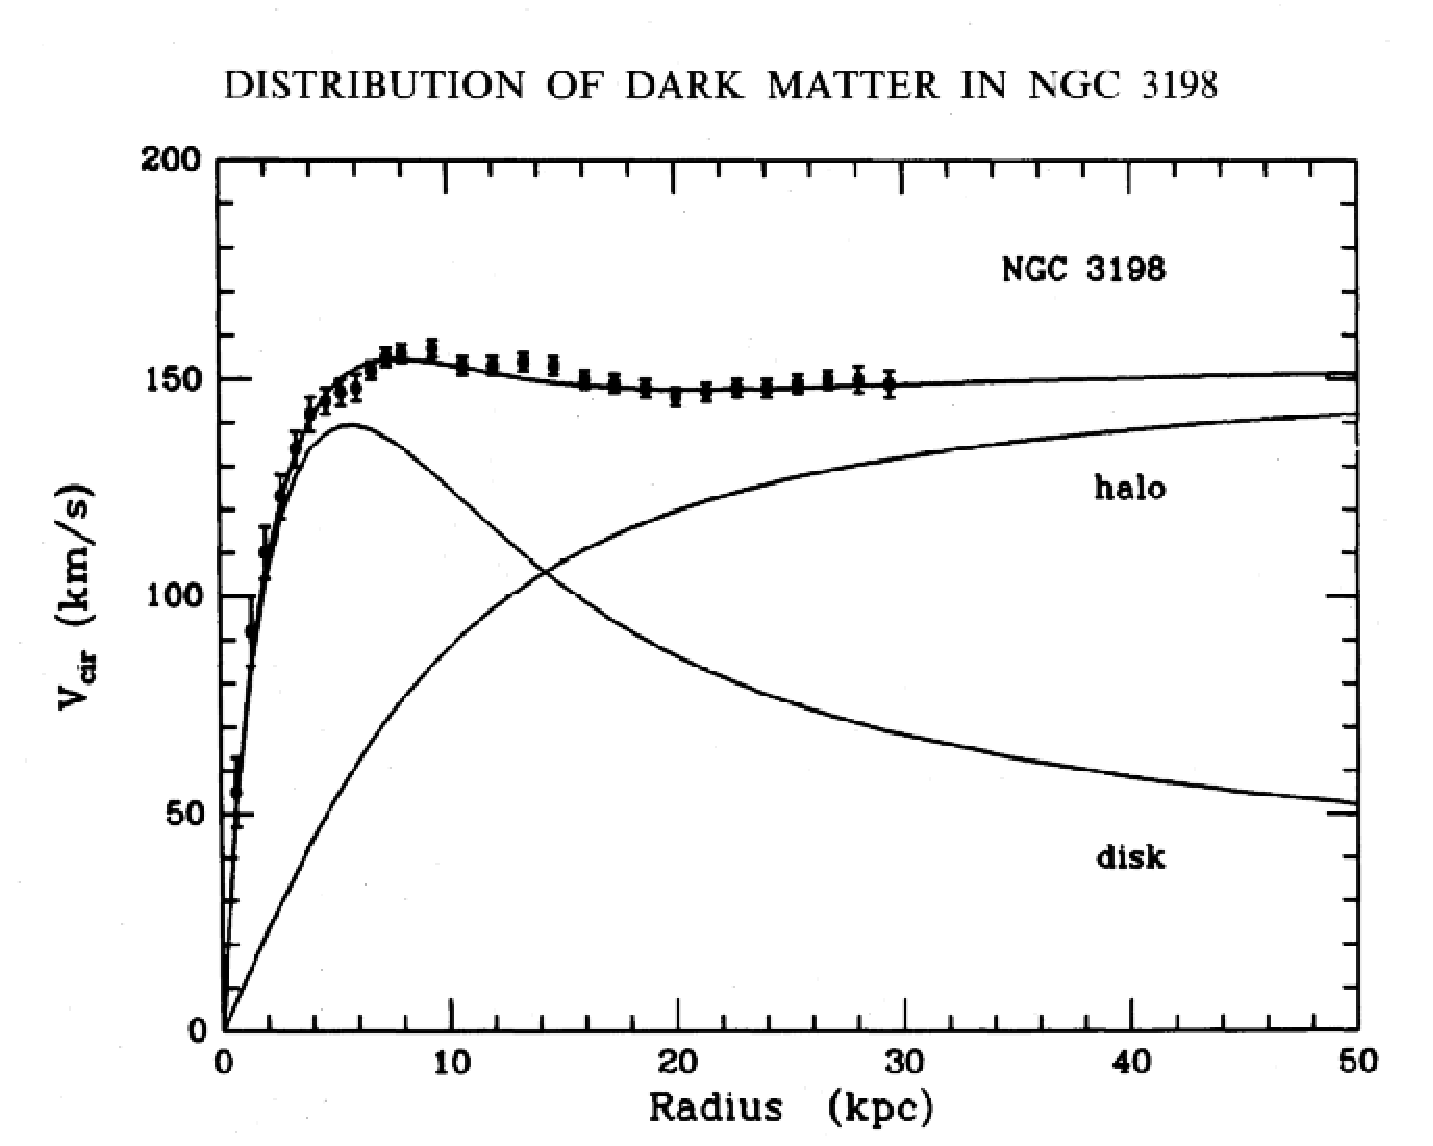
\includegraphics[width=\textwidth]{figure/Rot_vel_spir.pdf}
  \caption{Velocità di rotazione in una galassia a spirale}
  \label{vel_rot_spir}
\end{figure}
Si osserva che la velocità di rotazione galattica rimane costante fino a
distanze molto maggiori del raggio visibile $R_* \simeq 10$ kpc della galassia,
invece che diminuire con la distanza dal centro come $v_{rot}(r) \propto
r^{-1/2}$.  Questo comportamento è aspettato nell'ipotesi di esistenza della
sola materia visibile dalla 3$^a$ legge di Keplero.
\begin{figure}
  \centering{}
  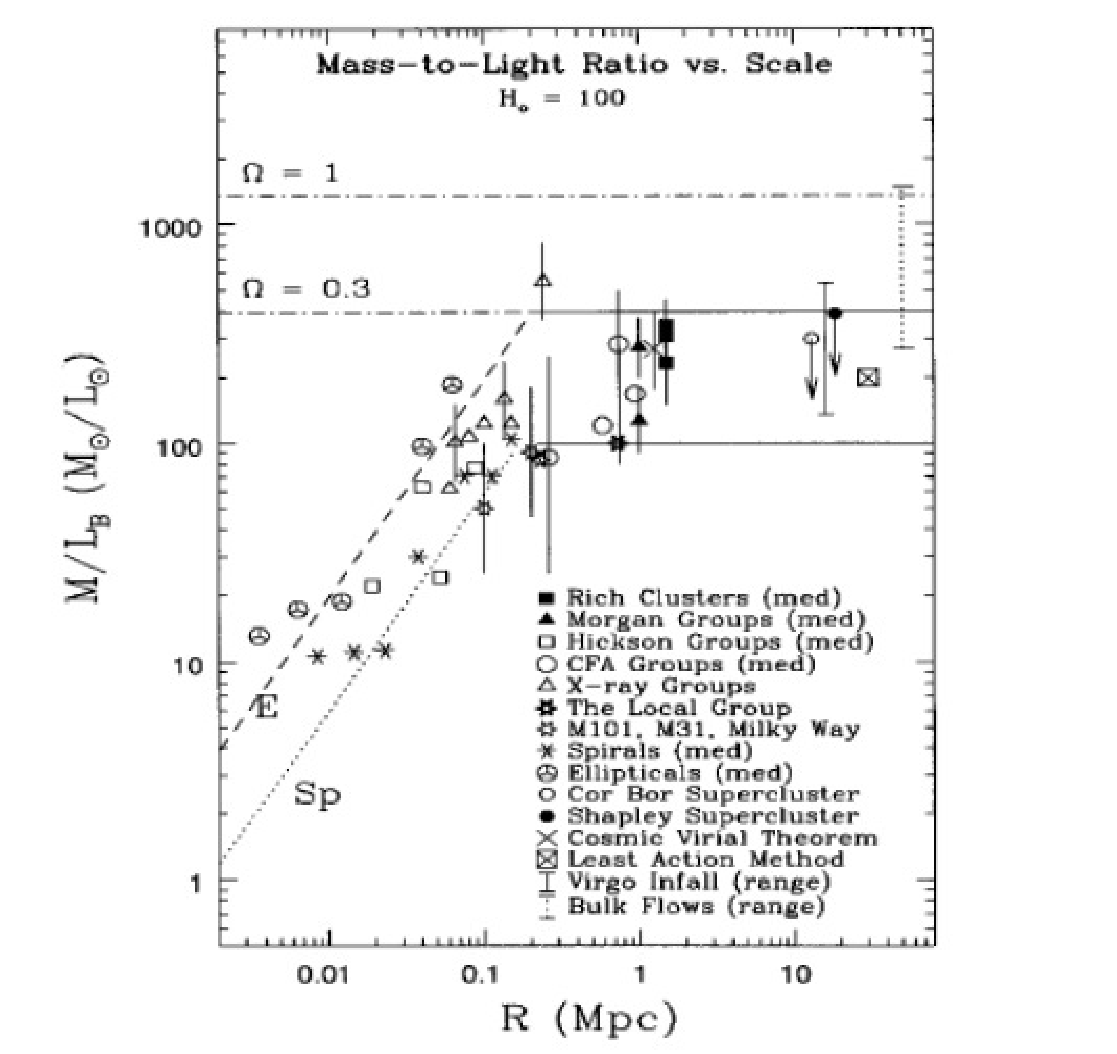
\includegraphics[width=0.7\textwidth]{figure/MoverL.pdf}
  \caption{Rapporto $M/L$ in funzione della scala}
  \label{moverl}
\end{figure}

Si deduce, quindi, che anche per le galassie a spirale $M_{din} = M_{*} +
M_{Dark}$. Se la materia oscura è distribuita con legge di densità $\rho_{Dark}
\simeq r^{-2}$ per $r>R_*$, si ha che $M_{din} \simeq r$ e quindi che
$V_{rot}(r) \propto cost$ fino a grandi distanze. Per le spirali si ottiene che
tipicamente $M_{Dark} \simeq 10 M_{*}$.

A partire dagli anni '80, osservazioni nella banda dei raggi X effettuate con
satelliti (Einstein, ROSAT, XMM, Chandra) hanno dimostrato l'esistenza di
materia oscura anche nelle galassie ellittiche (particolarmente in quelle di
grande massa) e nei clusters di galassie.  All'interno di questi sistemi
autogravitanti è presente gas diffuso (prevalentemente idrogeno ionizzato) che
si trova a temperatura $T_{gas }\simeq (0.1-1) \times 10^6$K nelle ellittiche e
$T_{gas }\simeq (3-10) \times 10^6$K nei clusters di galassie.

Il gas emette raggi X e la luminosità X totale dipende dalla massa totale di gas
$M_{gas}$ (trascurabile rispetto alla massa visibile $M_*$) e dalla temperatura
del gas $T_{gas}$.  Questa, a sua volta, attraverso il teorema del viriale e il
teorema di equipartizione dell'energia, $ m_{gas} v^2_{gas} /2 \simeq (3/2)
kT_{gas} \simeq m_{gas} G M_{din} /R$, dipende dalla massa dinamica $M_{din}$
oltre che dalle dimensioni $R$ del sistema considerato (ellittica o cluster di
galassie).  Anche in questo caso le osservazioni mostrano che $M_{din}$ è
maggiore della sola massa visibile in stelle.  Nel caso di M87, una galassia
ellittica di grande massa al centro del cluster Virgo, si trova $M_{Dark} \simeq
100 M_{*}$.
\begin{figure}
  \centering{}
  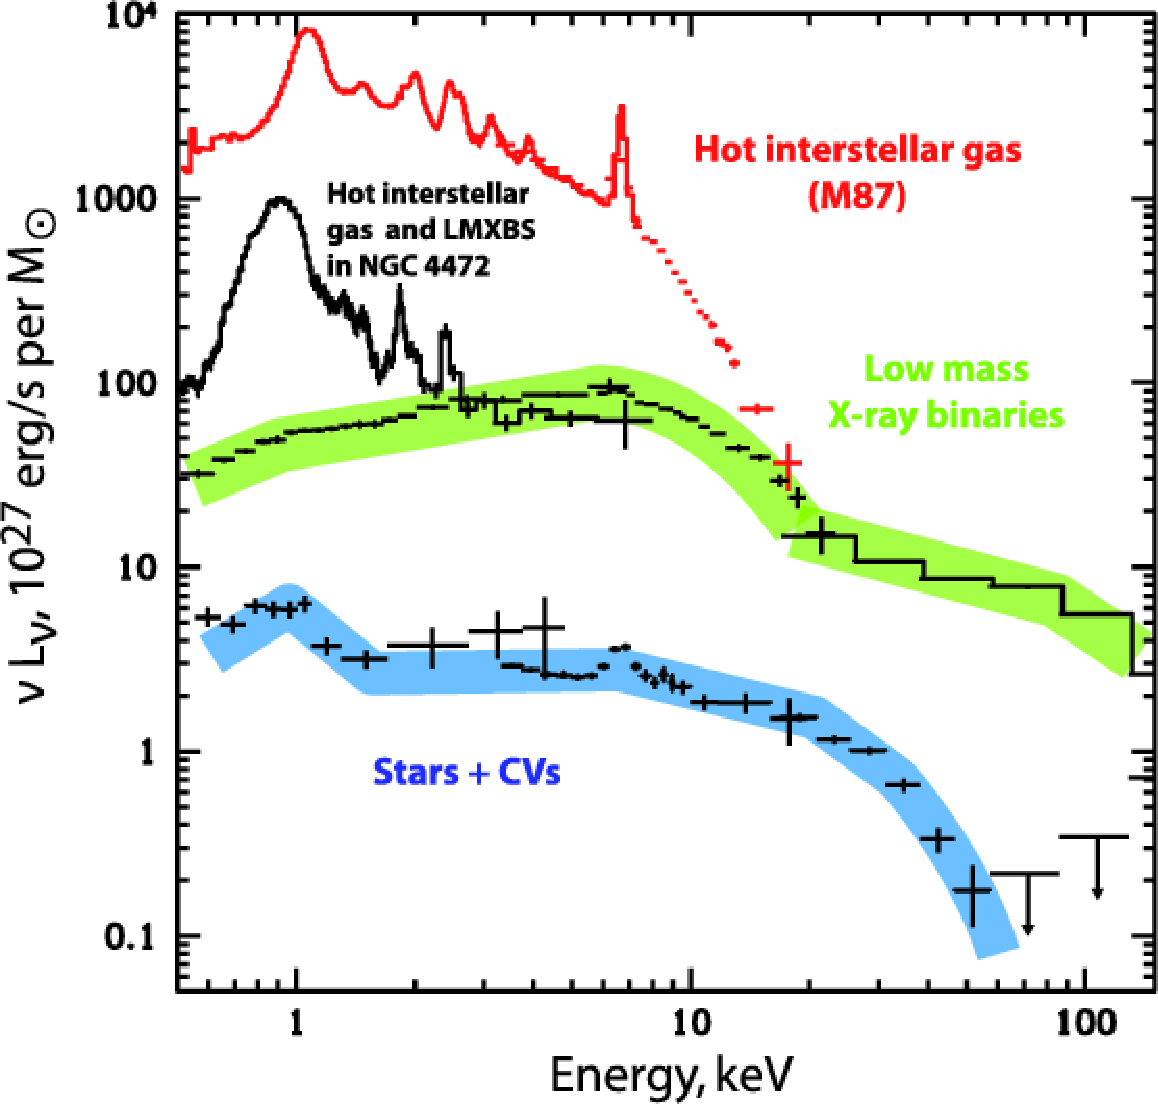
\includegraphics[width=0.7\textwidth]{figure/Xray_ellipt.pdf}
  \caption{Emissione di raggi X in alcune galassie ellittiche}
  \label{XRay_ell}
\end{figure}

\section{Principio Cosmologico}

\begin{figure}
  \centering{}
  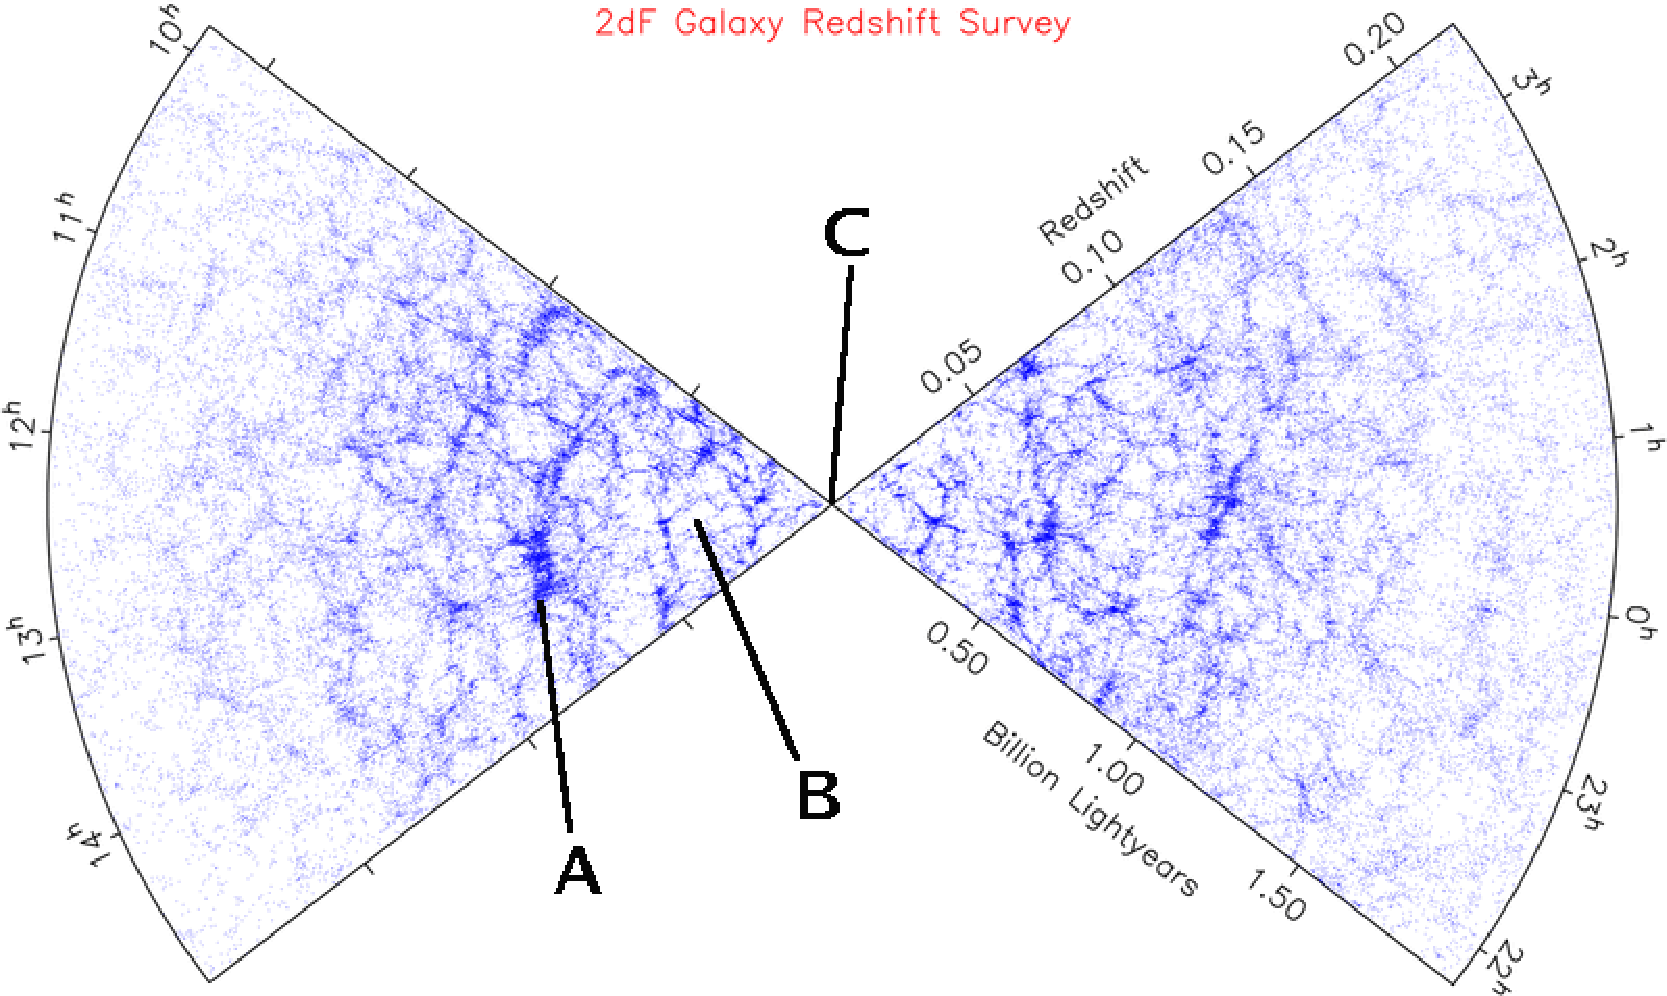
\includegraphics[width=\textwidth]{figure/2dFzcone.pdf}
  \caption{Catalogo 2dFz: distribuzione angolare di sorgenti}
  \label{cat_2d}
\end{figure}
\begin{figure}
  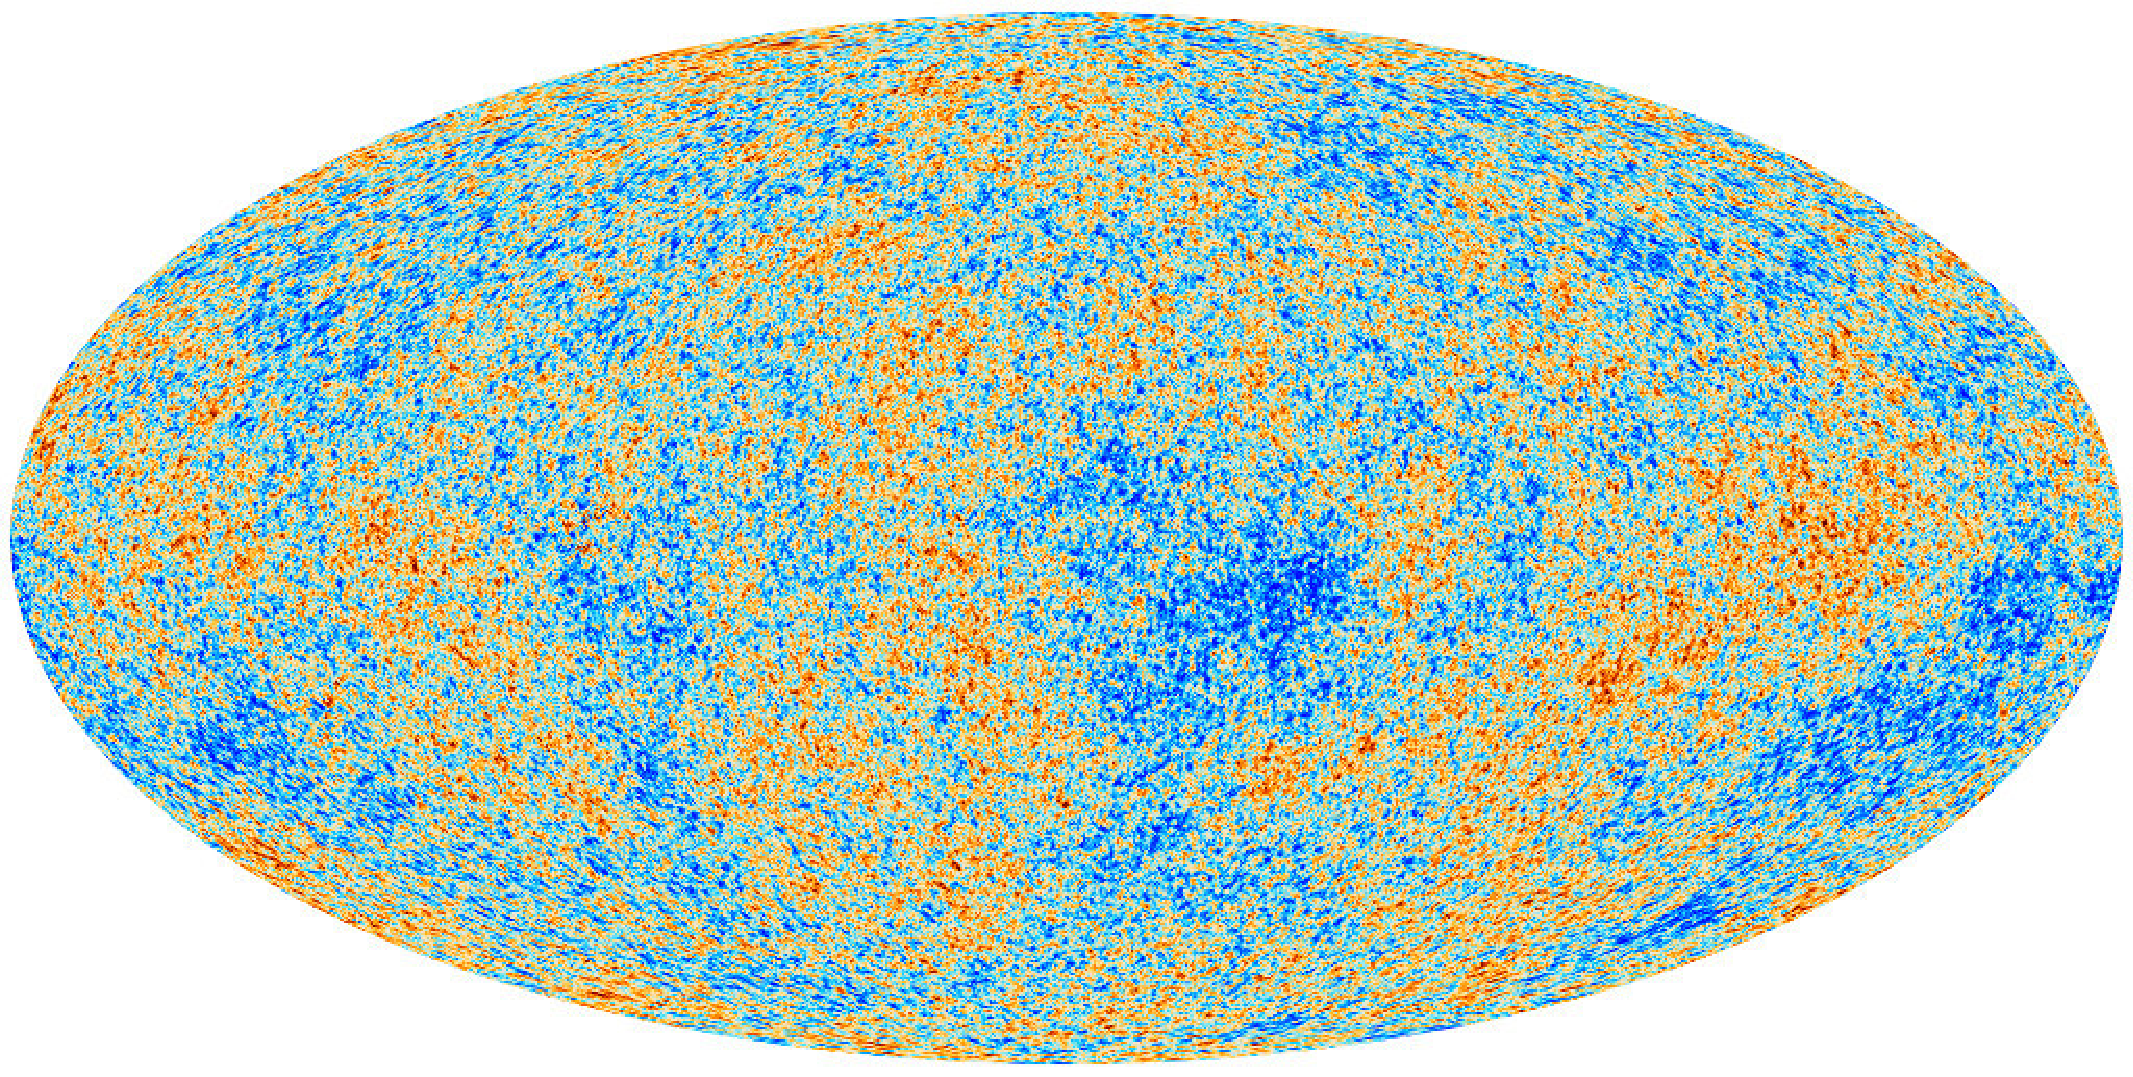
\includegraphics[width=\textwidth]{figure/Planck_CMB.pdf}
  \caption{Satellte Planck e temperatura della CMB}
  \label{sat_Planck}
\end{figure}
Il principio afferma che tutte le posizioni e tutte le direzioni direttamente
osservabili sono equivalenti: l'Universo mostra lo stesso aspetto e le stesse
proprietà fisiche in tutti i punti e in tutte le direzioni.  Le motivazioni di
carattere osservativo sono:
\begin{itemize}
\item non sono risultate anisotropie nella distribuzioni di sorgenti (nelle
  bande radio, ottico, UV, X e gamma) (vedi Fig. \ref{cat_2d}) su scala maggiore
  di 50-100 Mpc;
\item la dipendenza della velocità di recessione delle galassie con la distanza
  è la stessa in tutte le direzioni;
\item la radiazione di fondo cosmico è altamente isotropa (vedi
  Fig. \ref{sat_Planck}) poichè $\Delta T / T \simeq 10^{-5}$.
\end{itemize}

I costituenti elementari dell'Universo sono le galassie ed esiste una sequenza
di strutture (stelle, galassie, ammassi o gruppi, super-ammassi) che si arresta
sulla scala di $\simeq 100$ Mpc, oltre la quale l'Universo appare omogeneo ed
isotropo. Questa scala è molto minore della lunghezza di Hubble $R_H \simeq c
H_0$.

Comunque, non ogni oggetto può essere scelto come un buon osservatorio dal quale
verificare il Principio Cosmologico; si devono considerare solo traiettorie
fondamentali (una per ogni punto dello spazio-tempo) i cui punti possono servire
come origini di sistemi di riferimento di coordinate equivalenti: queste sono le
traiettorie di osservatori privilegiati ai quali lo spazio appare isotropo ed
omogeneo.  In prima approssimazione questi osservatori fondamentali coincidono
con le galassie in quanto ognuna di esse, a meno dei moti peculiari dovuti
all'appartenenza a sistemi autogravitanti, segue l'espansione di Hubble.

Il fatto che l'Universo presenta in ogni punto la stessa storia, fornisce una
sequenza assoluta di eventi temporali e quindi una base per definire un tempo
cosmico $t$.  Esso può essere definito come la densità o la temperatura della
CMB che variano in maniera monotona. Ad esempio per definire l'istante di
partenza di un ipotetico segnale inviato da noi verso civiltà lontane, noi
dovremmo solamente precisare che il segnale è stato inviato a $T_{CMB} =2.7$K.

\section{Geometria nell'Universo: metrica RW}

Dal punto di vista matematico il Principio Cosmologico pone restrizioni sulle
coordinate spazio-temporali ammissibili e la forma della metrica dello
spazio-tempo.

Introduciamo le coordinate spazio-temporali nel seguente modo: preliminarmente
una grandezza scalare che vari in maniera monotona (ad esempio la temperatura
del fondo cosmico nella banda delle microonde, $T_{CMB}$) fornisce un sequenza
assoluta di eventi che può essere usata per definire la scala temporale
nell'Universo.  Diremo che due eventi che accadano in posizioni differenti sono
\emph{simultanei} se una locale misura di $T_{CMB}$, effettuata al verificarsi
degli eventi, dà lo stesso valore.  L'insieme degli eventi simultanei, quindi
con stessa coordinata $t$, definisce una 3-superficie spaziale, che indichiamo
con $^{(3)}S(t)$, detta anche superficie di simultaneità.  Le coordinate
spaziali, ad esempio ($r, \theta , \phi$), sono introdotte per definire eventi
su $^{(3)}S(t)$.

Omogeneità dell'Universo significa che le condizioni fisiche sono identiche in
ogni punto di $^{(3)}S(t)$.  Quindi, queste 3-superfici devono avere curvatura
costante.

Isotropia dell'Universo significa che ad un dato tempo $t$, un osservatore
comovente con il fluido cosmologico (con le galassie) non può distinguere
direzioni spaziali attraverso misure locali.  Questo accade se e solo la
4-velocità delle galassie non ha componenti spaziali, se cioè le linee
d'Universo delle galassie sono lungo l'asse temporale.  Le galassie hanno quindi
coordinate spaziali fisse (comoventi) su $^{(3)}S$ e ciò nonostante (come
vedremo), all'aumentare di $t$, esse si allontanano l'una dall'altra a causa
dell'espansione: al crescere di $t$ la distanza tra le singole
galassie aumenta dello stesso fattore $R(t)$, mentre i rapporti di distanza
rimangono costanti.

In Cosmologia è conveniente introdurre le coordinate dello spazio-tempo in modo
che $g_{00}=-1$ e $g_{0i}=0$ (in particolare la seconda condizione permette di
sincronizzare gli orologi su di un percorso finito - vedi discussione
su~\textcite{landau:campi}).  Questo sistema è detto \emph{sincrono} e
l'espressione generale della metrica dello spazio-tempo assume la forma
\begin{equation}
  \dd\tau^2 \equiv \dd t^2 - \dd l^2 = \dd t^2 - ^{(3)}g_{ij}(t,\bm{x}) \dd x^i
  \dd x^j
\end{equation}
\begin{itemize}
\item La condizione $g_{00}=-1$ implica che per eventi che accadono nello stesso
  posto ($dx^i=0$) la differenza della coordinata temporale $dt$ misura il tempo
  proprio $d \tau$ trascorso tra i due eventi (il tempo segnato da un orologio
  che sia nello stesso posto).
\item La condizione $g_{0i}=0$ implica invece che le linee del tempo
  ($x^{\mu}(\tau)$ con $x^i=\text{cost}$) sono geodetiche dello spazio-tempo.
  Infatti poichè $g_{0i}=0$ si ha che $\tensor{\Gamma}{^{\mu}_{00}}=0$.  Con
  questo risultato (e per la condizione $dx^i=0$ per le linee del tempo),
  l'eq. della geodetica
  \begin{equation}
    \toder[2]{x^{\mu}} {\tau} + \tensor{\Gamma}{^{\mu}_{00}} \toder{x^0}{\tau}
    \toder{x^0}{\tau} = 0
  \end{equation}
  si riduce a
  \begin{equation}
    \toder[2]{x^{\mu}} {\tau} = 0
  \end{equation}
  da cui $x^{\mu}=\text{cost}$ è soluzione.
\item La stessa condizione $g_{01} =0$ implica inoltre che le linee del tempo
  sono ortogonali alle 3-superfici spaziali.  Cioè, se prendiamo un vettore
  orientato nel tempo $T^{\mu}=(1,0,0,0)$ ed uno orientato nello spazio
  $S^{\mu}=(0,S_x,S_y,S_z)$, si ha $T^{\mu} S_{\mu} = g_{0i} T^0 S^i =0$.

  Precedentemente abbiamo osservato che a causa dell'isotropia dell'Universo
  (rispetto ad osservatori fondamentali che coincidono con le galassie) la
  componente spaziale della 4-velocità delle Galassie deve essere nulla, quindi
  $V^{\mu}_G = \ltoder{x^{\mu}_G}{\tau} = (1,0,0,0)$.
\item Dalle considerazioni precedenti, segue allora che le coordinate delle
  Galassie e degli osservatori fondamentali sono fisse (labels) e che le loro
  linee d'universo sono dirette lungo l'asse del tempo risultando ortogonali
  alle 3-superfici spaziali.  Si osserva quindi che la condizione $g_{0i}=0$ è
  una condizione richiesta dall'isotropia di $^{(3)}S$.
\end{itemize}

Ora in Cosmologia, la parte spaziale della metrica $\dd
l^2=^{(3)}g_{ij}(t,\bm{x}) \dd x^i \dd x^j$ deve necessariamente avere la forma
\begin{equation}
  ^{(3)}g_{ij}(t,\bm{v}) = R^2(t) ^{3}\eta_{ij}(\bm{x})
  \label{metrica_eta}
\end{equation}
dove $^{(3)}\eta_{ij}(\bm x)$ è la metrica spaziale su una qualunque delle
3-superfici $^{(3)}S$. Infatti, il rapporto delle distanze tra due
galassie A e B
a tempi differenti non può:
\begin{itemize}
\item dipendere dalle coordinate degli estremi di A e B (omogeneità);
\item dipendere dalla direzione che connette A e B (isotropia);
\item dipendere dal modulo della distanza (per l'additività di piccole
  separazioni).
\end{itemize}
L'unica dipendenza possibile del rapporto di distanze è da una funzione del
tempo che indichiamo con $R(t)$.  Si ha allora
\begin{equation}
  \toder{l(t)}{l(t_I)} = R(t) \implies \dd l^2(t) =
  R^2(t)^{(3)}\eta_{ij}(\bm{x}) \dd x^i \dd x^j.
\end{equation}

L'isotropia attorno ad ogni punto di $^{(3)}S$ impone ulteriormente che il
termine $^{(3)}\eta_{ij}(\bm{x}) \dd x^i \dd x^j$ abbia la forma
\begin{equation}
  ^{(3)}\eta_{ij}(\bm{x}) \dd x^i \dd x^j = F(r) (\dd r^2 +r^2 \dd\Omega^2)
  \qquad\text{con}\qquad \dd\Omega^2 = \dd\theta^2 + \sin^2 \theta \dd\phi^2.
\end{equation}
Pertanto la forma completa della metrica dello spazio tempo in Cosmologia è
\begin{equation}
  \dd \tau^2 = \dd t^2 -  R^2(t) F(r) \left(\dd r^2 +r^2 \dd\Omega^2 \right)
  \label{forma_F(r)}
\end{equation}

Con il formalismo dei vettori di Killing si prova infine che la metrica deve
avere la forma stabilita da Robertson e Walker:
\begin{equation}
  d \tau^2 = dt^2 - R^2(t) \left[ \frac {dr^2}{1-kr^2} + r^2
    \left(d\theta^2+\sin^2 \theta d\phi^2\right) \right].
\end{equation}
dove $k$ è una costante che può assumere i valori $-1$, $0$, $+1$.  Questi 3
casi corrispondono a 3-superfici di curvatura costante negativa, nulla,
positiva.

\subsection{Vettori di Killing e metrica RW}

Un modo di determinare la funzione $F(r)$ in eq. \eqref{forma_F(r)} è di usare
l'omogeneità ed isotropia dello spazio, cioè la possibilità di spostare
l'origine delle coordinate in $^{(3)}S$ conservando la forma della metrica.

Consideriamo una trasformazione infinitesima di coordinate
\begin{equation}
  x^{\mu} \rightarrow x'^{\mu} = x^{\mu} + \epsilon \xi^{\mu}
  \qquad\text{con}\qquad \epsilon \ll 1
  \label{trasf_inf}
\end{equation}
che sia una isometria, cioè che lasci invariante in forma la metrica
\begin{equation}
  g'_{\mu \nu} (y) = g_{\mu \nu} (y)
  \label{inv_forma}
\end{equation}
quindi, eseguendo una trasformazione di coordinate la metrica rimane la stessa
funzione per ogni valore dell'argomento.

Vogliamo dimostrare che dalle condizioni in eq. \eqref{inv_forma} seguono le
eq. di Killing
\begin{equation}
  \xi_{\mu; \nu} + \xi_{\nu; \mu} = 0 \qquad\xi^0=0
  \label{eq_killing}
\end{equation}
La condizione $\xi^0=0$ è stata aggiunta perchè il tempo non è omogeneo.  Queste
eq. permetteranno di definire la metrica.

La dimostrazione procede nel modo seguente.  Preliminarmente, per una generica
trasformazione di coordinate $\xi^{\mu} \leftrightarrow \xi'^{\mu}$ il tensore
metrico covariante si trasforma come
\begin{equation}
  g_{\mu \nu} (x) =
  \frac{\partial x'^{\rho}  }{\partial x^{\mu}}
  \frac{\partial x'^{\sigma}}{\partial x^{\nu}}  g'_{\rho \sigma} (x')
  \label{13.1.2}
\end{equation}
Assumendo valida la condizione \eqref{inv_forma} di invarianza in forma della
metrica, possiamo sostituire nell'eq. \eqref{13.1.2} $g'_{\rho \sigma} (x')=
g_{\rho \sigma} (x')$
\begin{equation}
  g_{\mu \nu} (x) =
  \frac{\partial x'^{\rho}  }{\partial x^{\mu}}
  \frac{\partial x'^{\sigma}}{\partial x^{\nu}}  g_{\rho \sigma} (x')
\end{equation}
Si ha allora
\begin{equation}
  g_{\mu \nu} (x) =
  \left( \delta ^{\rho}_{\mu}   + \epsilon \frac{\partial \xi^{\rho}}{\partial
      x^{\mu}} \right)
  \left( \delta ^{\sigma}_{\nu} + \epsilon \frac{\partial \xi^{\sigma}}{\partial
      x^{\nu}}  \right)
  \left( g_{\rho \sigma} (x) + \frac{\partial g_{\rho \sigma}(x)}{\partial
      x^{\tau}} \epsilon \xi^{\tau} \right)
\end{equation}
e quindi al primo ordine in $\epsilon$,
\begin{equation}
  0 =  \frac{\partial \xi^{\rho}}{\partial x^{\mu}}  g_{\rho \nu} +
  \frac{\partial \xi^{\sigma}}{\partial x^{\nu}} g_{\mu \sigma} +
  \frac{\partial g_{\mu \nu}}{\partial x^{\tau}} \xi^{\tau}
  \label{eq_killing_2}
\end{equation}
che è una forma equivalente dell'eq. di Killing \eqref{eq_killing}.
Pongo ora $\xi^{\rho}   =  g^{\rho   \lambda} \xi_{\lambda}$ e
$\xi^{\sigma} =  g^{\sigma \lambda} \xi_{\lambda}$;
\begin{subequations}
  \begin{align}
    0 &= \frac{\partial ( g^{\rho   \lambda} \xi_{\lambda})  } {\partial
        x^{\mu}}  g_{\rho \nu}  +
        \frac{\partial ( g^{\sigma \lambda} \xi_{\lambda})  } {\partial x^{\nu}}
        g_{\mu \sigma} +
        \frac{\partial g_{\mu \nu}}{\partial x^{\tau}} \xi^{\tau} \\
    0 &=  \xi_{\lambda}     g_{\rho \nu}   \frac{\partial g^{\rho   \lambda}}
        {\partial x^{\mu}}  +
        g^{\rho \lambda}  g_{\rho \nu  } \frac{\partial \xi_{\lambda}     }
        {\partial x^{\mu}}  +
        \xi_{\lambda}     g_{\mu \sigma} \frac{\partial g^{\sigma \lambda} }
        {\partial x^{\nu}}  +
        g^{\sigma \lambda}g_{\mu \sigma} \frac{\partial \xi_{\lambda}      }
        {\partial x^{\nu}}   +
        \frac{\partial    g_{\mu \nu}}        {\partial x^{\tau}} \xi^{\tau}
  \end{align}
\end{subequations}
Per l'identità
\begin{equation}
  g^{\rho \lambda}g_{\rho \nu} =  \delta^{\lambda}_{\nu} \implies
  g_{\rho \nu} \frac{\partial g^{\rho _\lambda}}{\partial x^{\mu}} = -
  g^{\rho \lambda} \frac{\partial g_{\rho \nu}}{\partial x^{\mu}}
\end{equation}
abbiamo ora
\begin{equation}
 \begin{split}
   0 & = - \xi^{\rho} \frac{\partial g_{\rho \nu} } {\partial x^{\mu}} -
   \xi^{\sigma} \frac{\partial g_{\mu \sigma} } {\partial x^{\nu}} +
   \frac{\partial \xi_{\nu}} {\partial x^{\mu}} + \frac{\partial \xi_{\mu}}
   {\partial x^{\nu}} +
   \frac{\partial g_{\mu \nu}}{\partial x^{\tau}} \xi^{\tau} \\
   & = \frac{\partial \xi_{\nu}} {\partial x^{\mu}} + \frac{\partial \xi_{\mu}}
   {\partial x^{\nu}} + \xi^{\tau} \left[ \frac{\partial g_{\mu \nu} } {\partial
       x^{\tau}} - \frac{\partial g_{\tau \nu} } {\partial x^{\mu}} -
     \frac{\partial g_{\mu  \tau}} {\partial x^{\nu}} \right]\\
   & = \frac{\partial \xi_{\nu}} {\partial x^{\mu}} + \frac{\partial \xi_{\mu}}
   {\partial x^{\nu}} - 2 \xi_{\rho} \tensor{\Gamma}{^{\rho}_{\mu \nu}}
\end{split}
\end{equation}
o in maniera compatta
\begin{equation}
  0 = \xi_{\mu ; \nu} + \xi_{\nu ; \mu}.
\end{equation}
Consideriamo ora le componenti $rr$, $\theta \theta $ e $r \theta $ dell'eq. di
Killing nella forma \eqref{eq_killing_2}.  Osserviamo preliminarmente che
\begin{subequations}
  \begin{align}
    g_{\mu \nu} & = 0 \qquad\text{per}\qquad \mu \ne \nu, \\
     \parder{g_{\mu \nu}}{\phi}                  & = 0,   \\
                                         g_{r r} & = R^2(t) F(r), \\
    g_{\theta \theta}                            & = R^2(t) r^2.
  \end{align}
\end{subequations}
Per la componente $rr$ si ha:
\begin{equation}
  \frac{\partial g_{rr}}{\partial r} \xi^r +
  g_{rr}\frac{\partial \xi^r }{\partial r} +
  g_{rr}\frac{\partial \xi^r }{\partial r} =
  \frac{\partial F(r)}{\partial r} \xi^r +
  2 F(r) \frac{\partial \xi^r }{\partial r} = 0
  \label{eq_rr}
\end{equation}
Per la componente $\theta \theta$ si ha:
\begin{equation}
  \frac{\partial g_{\theta \theta}}{\partial r} \xi^r +
  g_{\theta \theta}\frac{\partial \xi^{\theta} }{\partial \theta} +
  g_{\theta \theta}\frac{\partial \xi^{\theta} }{\partial \theta} =
  \xi^r +  r \frac{\partial \xi^{\theta} }{\partial \theta} = 0
  \label{eq_thetatheta}
\end{equation}
Per la componente $r \theta$ si ha:
\begin{equation}
  \frac{\partial g_{r \theta}}{\partial r} \xi^r +
  g_{rr}\frac{\partial \xi^r       }{\partial \theta} +
  g_{\theta \theta} \frac{\partial \xi^{\theta}  }{\partial r} =
  F(r) \frac{\partial \xi^r}{\partial \theta}  +
  r^2  \frac{\partial \xi^{\theta} }{\partial r} = 0
  \label{eq_rtheta}
\end{equation}
Da eq. \eqref{eq_rr} si ha
\begin{equation}
  \frac{1}{\xi^r} \frac{\partial \xi^r}{\partial r} =-\frac{1}{2 F(r)}
  \frac{\partial F(r)}{\partial r}
\end{equation}
la cui soluzione è $\ln \xi^r =-(1/2) \ln F(r) + \text{costante}$ (rispetto a
\(r\)), cioè
\begin{equation}
  \xi^r = C(\theta, \phi) \frac{1}{\sqrt {F(r)}}
  \label{367}
\end{equation}
Da eq. \eqref{eq_thetatheta} si ha
\begin{equation}
  \frac{\partial^2 \xi^{\theta} }{\partial r \partial \theta} = -
  \frac{\partial}{\partial r } \left(\frac{\xi^r}{r}\right)
  \label{368}
\end{equation}
e da eq. \eqref{eq_rtheta}
\begin{equation}
  \frac{\partial^2 \xi^{\theta} }{\partial \theta \partial r} = -
  \frac{\partial}{\partial \theta } \left( \frac{F(r)}{r^2} \frac{\partial
      \xi^r}{\partial \theta}\right)
  \label{369}
\end{equation}
Dalle eq. \eqref{368} e \eqref{369} si ha
\begin{equation}
  F(r) \frac{\partial^2 \xi^r}{\partial \theta^2} +
  r^2 \left( \frac{\xi^r}{r^2} -\frac{1}{r} \frac{\partial \xi^r}{\partial r}
  \right) = 0
\end{equation}
e sostituendo la \eqref{367} nella precedente,  si ottiene
\begin{equation}
  \frac{1}{C} \frac{d^2 C(\theta,\phi)}{d \theta^2} =
  \frac{r^2}{\sqrt{ F(r)}} \frac{d}{dr} \left( \frac{1}{r \sqrt{F(r)}}\right)=
  \text{costante} \equiv D
\end{equation}
Dall'uguaglianza
\begin{equation}
  \frac{1}{C} \frac{d^2 C(\theta,\phi)}{d \theta^2} = D
\end{equation}
segue che necessariamente $D=-1$
\begin{equation}
  \begin{split}
    C(\theta,\phi) \propto \cos \theta & \implies
    \frac{1}{C} \frac{d^2 C(\theta,\phi)}{d \theta^2} = -1 \\
    & \implies
    \frac{r^2}{\sqrt{ F(r)}} \frac{d}{dr} \left( \frac{1}{r \sqrt{F(r)}}\right)=
    -1
  \end{split}
\end{equation}
L'eq. differenziale per $F(r)$ può essere posta nella forma
\begin{equation}
  \frac{1}{r\sqrt{F(r)}}\toder{}{r} \left(\frac{1}{r \sqrt{F(r)}}\right)= -
  \frac{1}{r^3}
\end{equation}
o, equivalentemente,
\begin{equation}
  \frac{1}{2} \dd \left( \frac{1}{r \sqrt{F(r)}} \right)^2 =
  \frac{1}{2} \dd \left(\frac{1}{r^2}\right)
\end{equation}
che si integra facilmente
\begin{equation}
  F(r) \propto \frac{1}{1+E r^2}
\end{equation}
dove $E$ è un costante.  Ridefinendo la coordinata radiale $r$ si può scrivere
infine
\begin{equation}
  F(r) \propto \frac{1}{1+k r^2}
\end{equation}
dove $k$ può assumere i valori +1, 0, -1.

\subsection{Coordinate spaziali}

Con riferimento all'eq. \eqref{metrica_eta} vogliamo ricavare la forma della
matrice $^{(3)}\eta_{ij}$.

\subsubsection{Caso $k=+1$}

L'analoga superficie in 2 dimensioni è la 2-sfera che possiamo visualizzare
nello spazio 3-dimensionale con metrica euclidea
\begin{equation}
  dl^2 = dx^2+dy^2+dz^2
\end{equation}
Appartengono alla 2-sfera i punti di coordinate $(x,y,z)$ con
\begin{equation}
  x^2+y^2+z^2=R^2
\end{equation}
con il cambiamento di variabili
\begin{equation}
  \begin{split}
    & x=R \sin \theta \cos \phi~~~~~~~~~~~~~~~~~~ 0\le \theta \le \pi \\
    & y=R \sin \theta \sin \phi~~~~~~~~~~~~~~~~~~0\le \theta \le 2 \pi \\
    & z=R \cos \theta~~~~~~~~~~~~~~~~~~~~~~~~~~~0\le \theta \le \pi
    \label{coord_sfer}
\end{split}
\end{equation}
si ha
\begin{equation}
dl^2 = R^2(d\theta^2 + \sin^2 \theta d\phi^2).
\end{equation}

In maniera analoga per la 3-sfera nello spazio euclideo 4-dimensionale si ha
\begin{subequations}
  \begin{gather}
    \dd l^2 = \dd x^2 + \dd y^2 + \dd z^2 + \dd w^2 \\
    x^2+y^2+z^2+w^2=R^2
  \end{gather}
\end{subequations}
da cui
\begin{equation}
  0 = 2 x dx + 2 y dy+ 2z dz + 2w dw \implies dw = - \frac {xdx+ydy+zdz}{\left(
      R^2-x^2-y^2-z^2 \right)^{1/2}}
\end{equation}
e quindi
\begin{equation}
dl^2 = dx^2+dy^2+dz^2 - \frac{ \left( xdx+ydy+zdz \right)^2}{\left(
    R^2-x^2-y^2-z^2 \right)}.
\end{equation}
Introduciamo le coordinate polari sferiche:
\begin{equation}
  \begin{split}
    & x=R \sin \chi \sin \theta \cos \phi                 \\
    & y=R \sin \chi \sin \theta \sin \phi~~~~~~~~~~~~~~~~~~~~~0\le \phi  \le 2 \pi \\
    & z=R \sin \chi \cos \theta~~~~~~~~~~~~~~~~~~~~~~~~~~~~~~0\le \theta \le \pi \\
    & w=R \cos \chi ~~~~~~~~~~~~~~~~~~~~~~~~~~~~~~~~~~~~~~0\le \chi \le \pi
\end{split}
\end{equation}
si ha quindi
\begin{subequations}
  \begin{align}
    x^2 + y^2 + z^2     & = R^2 \sin^2 \chi \\
    x dx + y dy + z dz  & = R^2 \sin \chi \cos \chi d \chi \\
    dx^2 + dy^2 + dz^2 & = R^2 \cos^2 \chi d \chi^2 + R^2 \sin^2 \chi d \theta^2
                         + R^2 \sin^2 \chi \sin^2 \theta d \phi^2
  \end{align}
\end{subequations}
da cui segue
\begin{equation}
  dl^2 = R^2 \left[ d \chi^2 + \sin^2 \chi \left( d \theta^2 + \sin^2 \theta d
      \phi^2 \right) \right]
\end{equation}
e posto infine $k=1$
\begin{equation}
  r= \sin \chi \implies d \chi^2 = \frac{dr^2}{1-kr^2}
\end{equation}
si ha la parte spaziale della metrica RW
\begin{equation}
  dl^2 = R^2 \left[ \frac{dr^2} {1-kr^2} + r^2 (d \theta^2+\sin^2 \theta d\phi^2) \right]
\end{equation}

Le 2-superfici a $\chi$ fissato sono 2-sfere, su cui variano $\theta$ e $\phi$,
di raggio $R \sin \chi$.  Su queste 2-sfere la distanza è $dl^2 = R^2 \sin^2
\chi (d \theta^2+\sin^2 \theta d\phi^2)$, quindi
\begin{equation}
  \sqrt{^{(2)}\eta } = R^2 \sin\chi \sin \theta \implies
  ^{(2)}V= \int_0^{\pi} \int_0^{2 \pi} R^2 \sin\chi \sin \theta d \phi d \theta =
  4\pi R^2 \sin \chi
\end{equation}
L'intero volume della 3-sfera è
\begin{equation}
  \sqrt{^{(3)}\eta } = R^3 \sin^2 \chi \sin \theta \implies
  ^{(3)}V = \int_0^{\pi} \int_0^{\pi} \int_0^{2 \pi}  R^2 \sin^2 \chi \sin \theta d
  \phi d \theta d \chi =  2 \pi^2 R^3
\end{equation}

\subsubsection{Caso $k=+0$}

È lo spazio euclideo tridimensionale descitto in coordinate polari sferiche $r=R
\chi$
\begin{equation}
  \begin{split}
    & x=R \chi \sin \theta \cos \phi~~~~~~~~~~~~~~~~~~~   0 \le \chi < \infty \\
    & y=R \chi \sin \theta \sin \phi~~~~~~~~~~~~~~~~~~~~0\le \phi  \le 2 \pi \\
    & z=R \chi \cos \theta~~~~~~~~~~~~~~~~~~~~~~~~~~~~~0\le \theta \le \pi \\
  \end{split}
\end{equation}
e distanza data da
\begin{equation}
  dl^2 = R^2 \left[ d \chi^2 + \chi^2 \left( d \theta^2+\sin^2 \theta d\phi^2
    \right) \right]
\end{equation}
L'intera 3-superficie ha volume infinito.

\subsubsection{Caso $k=-1$}

L'analoga superficie in 2-dimensioni è l'iperboloide di rivoluzione attorno
all'asse $z$ di eq.
\begin{equation}
  z^2 - (x^2+y^2) = R^2
\end{equation}
che visualizziamo immersa nel 3-spazio con metrica pseudo-euclidea
\begin{equation}
  dl^2 = dz^2-(dx^2+dy^2)
\end{equation}

Nel caso della 3-superficie con curvatura negativa abbiamo
\begin{equation}
  w^2 - (x^2+y^2+z^2) = R^2
\end{equation}
e la metrica diventa
\begin{equation}
  dl^2 = dw^2 - (dx^2+dy^2+dz^2)
\end{equation}
Le coordinate sono ora
\begin{equation}
  \begin{split}
    & x=R \sinh \chi \sin \theta \cos \phi~~~~~~~~~~~~~~~~  \\
    & y=R \sinh \chi \sin \theta \sin \phi~~~~~~~~~~~~~~~~~~~0\le \phi  \le 2 \pi \\
    & z=R \sinh \chi \cos \theta~~~~~~~~~~~~~~~~~~~~~~~~~~~~~0\le \theta \le \pi \\
    & w=R \cosh \chi ~~~~~~~~~~~~~~~~~~~~~~~~~~~~~~~~~~~~~  ~0\le \chi \le \infty    \\
  \end{split}
\end{equation}
Procedendo in modo analogo al caso $k=+1$ si ha
\begin{equation}
  dl^2 = R^2 \left[ d \chi^2 + \sinh^2 \chi \left( d \theta^2 + \sin^2 \theta d
      \phi^2 \right) \right]
\end{equation}
e posto $k=-1$
\begin{equation}
  r= \sinh \chi \implies d \chi^2 = \frac{dr^2}{1-kr^2}
\end{equation}
si ha infine
\begin{equation}
  dl^2 = R^2 \left[ \frac{dr^2} {1-kr^2} + r^2 (d \theta^2+\sin^2 \theta
    d\phi^2) \right].
\end{equation}
L'intero volume $^{(3)}V= 4 \pi R^2 \sinh^2 \chi$ è infinito.

\section{Tensore energia-impulso dell'Universo}

Come in Relatività Generale il contenuto dell'Universo (materia, radiazione,
raggi cosmici, campi magnetici, \dots) è descritto dal tensore-energia impulso
$T{\mu \nu}$.  Il Principio Cosmologico richiede che questo tensore abbia la
forma richiesta per un fluido perfetto (omogeneo ed isotropo rispetto agli
osservatori comoventi).

Dalla Relatività Speciale e il Principio di Generale Covarianza segue
\begin{equation}
  T^{\mu \nu} = ( p+ \rho) U^{\mu} U^{\nu} + p g^{\mu \nu}
\end{equation}
in cui $\rho= \rho(t)$ e $p= p(t)$ sono densità di energia e pressione totali
(proprie) misurate da osservatori comoventi.  Esse dipendono solamente dal tempo
cosmico $t$ e non dalle coordinate spaziali.

Con riferimento ai componenti dell'Universo, materia e radiazione si ha
\begin{subequations}
  \begin{align}
  \rho(t) &= \rho_m(t) + \rho_r(t), \\
  p(t) &=p_m(t)+p_r(t).
  \end{align}
\end{subequations}

Con l'uso della meccanica statistica si dimostra che
\begin{subequations}
  \begin{align}
    \rho_m &= \rho_{rm}+ u_m \\
    u_m &= \frac{p_m}{\gamma -1} \\
    \rho_{rm} &= n_m M_m c^2 \\
    p_m &\simeq n_m M_m v^2
  \end{align}
\end{subequations}
dove con $n_m$ abbiamo indicato la densità in numero di particelle, di stessa
massa $M_m$, con $u_m$ l'energia interna (termica), con $\gamma$ il rapporto di
calori specifici --- $\gamma=5/3$ (oppure $4/3$) per particelle
non-relativistiche (o relativistiche) --- e con $v$ la velocità media delle
particelle.  Nel caso di basse velocità, $v<c$, si ha $\rho_m \gg p$ e quindi si
può porre per la materia $p_m \simeq u_m \simeq 0$.

Per quanto riguarda la radiazione si ha sempre
\begin{equation}
  p_r = \frac{\rho_r}{3}
\end{equation}
e per la CMB, che ha distribuzione di corpo nero alla temperatura $T_{CMB}$,
\begin{equation}
  \rho_{CMB} = a T^4_{CMB}
\end{equation}

All'istante attuale (escludendo la Dark Energy) il maggior contributo alla
densità totale di energia nell'Universo $\rho_0$ è dato dalla materia
\begin{equation}
  \rho_0 \simeq \rho_m(0)
\end{equation}
poichè $\rho_m(0) > \rho_*(t_0) \simeq 10^{-31}$ gr cm$^{-3}$ e $\rho_r(t_0)$ è
dominata dai fotoni della CMB per i quali $\rho_{CMB}(t_0) \simeq 10^{-34}$ gr
cm$^{-3}$.

Inoltre, poiché i moti peculiari della materia (le galassie) avvengono a bassa
velocità ($\langle v_{G}\rangle \simeq 1000$ km s$^{-1}$) si può porre $p_0=0$
nell'Universo (in un modello senza DE).

In realtà indietro nel tempo l'Universo ha attraversato una fase in cui era la
radiazione a dominare.  Infatti l'applicazione della Relatività Speciale e del
Principio di Equivalenza implica che il tensore energia-impulso deve soddisfare
l'identità $\tensor{T}{^{\mu \nu}_{;\nu}}=0$ e per
$\nu=0$~\parencite[414]{weinberg:gravitation}
\begin{equation}
  R^3 \frac{dp}{dt} = \frac{d}{dt} \left[R^3 \left( \rho +p \right) \right]
\end{equation}
Questa eq. si può porre anche nella forma ($d/dt \equiv {\dot R} d/dR$)
\begin{equation}
  \frac{d}{dR} \left( \rho R^3 \right)  = -3pR^2
  \label{eq_cons}
\end{equation}
da cui è evidente che
\begin{subequations}
  \begin{align}
    \rho_m  & \simeq R^{-3} \qquad\text{se}\qquad p_m=0 \quad\text{(era
              materia)} \\
    \rho_r  & \simeq R^{-4} \qquad\text{se}\qquad p_r=\frac{\rho_r}{3}
              \quad\text{(era radiazione)}
  \end{align}
\end{subequations}

Allora ad ogni tempo cosmico abbiamo
\begin{subequations}
  \begin{align}
    \rho_m (t) &= \rho_m(t_0) \left( \frac {R(t_0)} {R(t)} \right)^3  \\
    \rho_r (t) &= \rho_r(t_0) \left( \frac {R(t_0)} {R(t)} \right)^4
  \end{align}
\end{subequations}
L'ultima relazione, poiché per la radiazione di fondo cosmico $\rho_r \propto
T^4_{CMB}$, implica che $T_{CMB}(t)$ cambia nel tempo secondo la relazione
\begin{equation}
  T_{CMB}(t) = T_{CMB}(t_0) \left( \frac {R(t_0)} {R(t)} \right).
\end{equation}
Quindi l'Universo oggi è dominato dalla materia, ma poichè indietro nel tempo
$\rho_r(t)$ cresce più velocemente di $\rho_m(t)$, esisterà nel passato un'era
della radiazione in cui $\rho(t) \simeq \rho_r(t)$.

Con riferimento all'epoca in cui le galassie sono già formate, possiamo definire
una densità di corrente di galassie
\begin{equation}
  J^{\mu}_{~G}(t) = n_G(t) U^{\mu}
  \label{154}
\end{equation}
dove $n_G(t)$ è la densità propria di galassie e $U^{\mu}=(1,0,0,0)$ è la
4-velocità delle galassie.  La conservazione del numero di galassie sarà
espressa dalla relazione
\begin{equation}
  J^{\mu}_{G~~;\mu} \equiv \frac{1}{\sqrt{g}} \frac{\partial}{\partial t}
  (\sqrt{g} n_G)
\end{equation}
Il determinante della metrica RW (cambiato di segno) è
\begin{equation}
  g=R^6(t) r^4 (1-kr^2)^{-1} \sin \theta ^2
\end{equation}
e quindi l'eq. \eqref{154} diventa
\begin{equation}
  n_G(t) R^3(t) = \text{costante}.
\end{equation}
Nota che $n_G(t)$ è la densità in numero di galassie per unità di volume
proprio\footnote{L'osservatore comovente usa una misura di lunghezza $l$ che non
  varia con l'espansione dell'Universo, conta il numero totale $N_G$ di galassie
  entro un volume proprio di dimensioni $l^3$ e calcola $n_G = N_G/l^3$.}  ed
esso diminuisce (aumenta) a seconda che l'Universo si espande (si contrae).
Allo stesso tempo $n_G(t) R^3(t)$ è la densità di galassie per unità di volume
comovente, che rimane costante nel tempo.

Allora la dipendenza da $R(t)$ delle densità $\rho_m(t)$ e $\rho_r(t)$ ha una
semplice interpretazione.  Se l'Universo è in espansione, la densità propria di
oggetti (galassie o fotoni) diminuisce come $R^{-3}$.  Per la materia non
relativistica, la cui densità di energia è dominata dalla massa a riposo, si ha
$\rho_m (t) \simeq n_G (t) M_m c^2 \simeq R^{-3}$.  Per quanto riguarda la
radiazione, il numero proprio di fotoni $n_{\gamma} \simeq R^{-3}$, ma la
densità di energia $\rho_r \simeq n_{\gamma} E_{\gamma}$ varia come $\simeq
R^{-4}$, poichè l'energia di ciascun fotone $E_{\gamma} = hc/\lambda$ scala come
$\simeq R^{-1}$.

\section{Distanza propria}

La distanza tra due galassie, ad esempio la nostra Galassia ad $r=0$ ed una
galassia esterna con coordinata radiale $r_1$, si calcola ad ogni tempo dalla
metrica RW ponendo $dt=0$, il che esprime la condizione di contemporameità, e $d
\theta = d \phi =0$, come è sempre possibile fare con una opportuna orientazione
del sistema di coordinate.  In questo modo si ottiene
\begin{equation}
  D_P(t) = R(t) \int_0^{r_1} \frac{dr}{\sqrt{1-kr^2}} \equiv R(t) f(r_1)
  \label{dprop}
\end{equation}
dove $f(r_1)$ è data da
\begin{equation}
  f(r_{1}) =
  \begin{cases}
    \arcsin r_{1}  & \text{se } k = 1, \\
    r_{1}        & \text{se } k = 0, \\
    \arcsinh r_{1} & \text{se } k = -1.
  \end{cases}
\end{equation}
Per piccoli valori di $r_1\ll 1$ si ha
\begin{subequations}
  \begin{align}
    \arcsin r_1 &= r_1 +\frac{r_1^3}{6}  \simeq r_1 \\
    \arcsinh r_1 &= r_1 -\frac{r_1^3}{6}  \simeq r_1
  \end{align}
\end{subequations}
e la distanza propria diventa:
\begin{equation}
  D_P(t) = R(t) r_1 + O(r_1^3) \qquad\text{se}\qquad r_1 \ll 1.
\end{equation}

Dal punto di vista osservativo la distanza propria $D_P(t)$ non ha significato
fisico perchè le misure di distanza eseguibili non possono avvenire a uguale
tempo cosmico $t$.  La misura di distanze in Cosmologia presuppone la
propagazione di segnali elettromagnetici che sono emessi al tempo $t_1$ da una
galassia esterna (nella posizione $r_1$) e che si propagano fino a noi (in
$r=0$) che li riceviamo all'istante $t_0>t_1$.

Si definisce \emph{red-shift cosmologico} la quantità
\begin{equation}
  z = 1 + \frac{R(t_0)}{R(t)}.
\end{equation}
Si stabilisce così una corrispondenza biunivoca tra tempo $t$ e red-shift $z$:
l'istante attuale $t_0$ corrisponde a $z=0$; indietro nel tempo $R(t)$ decresce
così che $z$ cresce, e per $t \to 0$ si ha $z \to +\infty$.  Gli oggetti più
lontani (e più vecchi) che noi oggi osserviamo sono i QSOs che si trovano $z
\simeq 5$.  Il tempo corrispondente a tale valore di $z$ risulta una frazione
apprezzabile dell'età dell'Universo.

Derivando rispetto al tempo la relazione \eqref{dprop} e prendendo il risultato
al tempo attuale, si trova in modo formale la legge di Hubble
\begin{equation}
  V_H = \frac {dD_P(t)}{dt}|_{t=t_0} = \dot{R}_0 f(r_1) = H_0 D
\end{equation}
dove si è definita la costante di Hubble
\begin{equation}
  H_0=\frac{\dot{R}_0}{R_0}.
\end{equation}

\section{Red-shift cosmologico}

Consideriamo un segnale elettromagnetico emesso al tempo $t=t_1$ da una galassia
lontana, con coordinata radiale $r=r_1$.  Il segnale è da noi ricevuto in $r=0$
al tempo $t_0>t_1$.  Dal Principio di Equivalenza la velocità di propagazione è
pari a $c$, e quindi $d \tau= 0$.  Se orientiamo gli assi in modo che $d \theta
= d \phi=0$, dalla metrica RW si ha
\begin{equation}
  dt = R(t) \frac{dr}{\sqrt{1-kr^2}}
\end{equation}
e integrando (osserva che $dr<0$)
\begin{equation}
  \int_{t_1}^{t_0} \frac{dt}{R(t)} = \int_0^{r_1} \frac{dr}{\sqrt{1-kr^2}}
  \equiv f(r_1)
\end{equation}
Si stabilisce quindi una corrispondenza implicita tra $r_1$, $t_1$, $t_0$.

Consideriamo ora una sola lunghezza d'onda: la prima cresta d'onda parte al
tempo $t_1$ e arriva al tempo $t_0$ dato da
\begin{equation}
  \int_{t_1}^{t_0} \frac{dt}{R(t)} =  f(r_1).
\end{equation}
La cresta successiva parte al tempo $t_1+\Delta t_1$ e arriva al tempo $t_0+
\Delta t_0$ dato ancora da
\begin{equation}
  \int_{t_1+ \Delta t_1}^{t_0+ \Delta t_0} \frac{dt}{R(t)} =  f(r_1).
\end{equation}
Da queste due relazioni si ricava l'uguaglianza
\begin{equation}
  \int_{t_1}^{t_0} \frac{dt}{R(t)} =  \int_{t_1+ \Delta t_1}^{t_0+ \Delta t_0}
  \frac{dt}{R(t)}
\end{equation}
che implica
\begin{equation}
  \int_{t_1}^{t_1+\Delta t_1} \frac{dt}{R(t)} =  \int_{t_0}^{t_0+ \Delta t_0}
  \frac{dt}{R(t)}
  \label{169}
\end{equation}

Ora i tempi $\Delta t_1= 1/\nu_1$ e $\Delta t_0 = 1/\nu_0$ corrispondono a
periodi del segnale elettromagnetico in partenza e in arrivo che, anche
considerando le onde di lunghezza d'onda massima che arrivano a terra (nel radio
$\Delta t \simeq 10^{-7}$ sec), sono estremamente più piccoli dei tempi su cui
varia $R$.  Perciò possiamo approssimare l'eq. \eqref{169} con
\begin{equation}
  \frac{\Delta t_1}{R_1} = \frac{\Delta t_0}{R_0}
\end{equation}
o, equivalentemente,
\begin{equation}
  \frac{\nu_0}{\nu_1} = \frac{\lambda_1}{\lambda_0}= \frac{R(t_1)}{R(t_0)}
  \implies \lambda \sim R(t).
\end{equation}
per cui la lunghezza d'onda della radiazione di fondo cosmico scala come $R$. In
termini del red-shift $z$ si ha
\begin{equation}
1+z \equiv \frac {R(t_0)} {R(t_1)} = \frac{\lambda_0} {\lambda_1}
\end{equation}
Le misure di red-shift cosmologico mostrano che $z>0$ e pertanto che l'Universo
oggi è in espansione.

Il red-shift è un effetto di scala e la sua legge generale è $\lambda \sim R$.
Comunque, per oggetti vicini esso si riduce all'effetto Doppler.  Infatti,
ponendo $\Delta t = t_0-t_1 >0 $, in prima approssimazione si ha
\begin{equation}
  1+z = \frac{R_0} {R(t_0-\Delta t)} \simeq \frac{R_0} {R_0 -\dot{R}_0 \Delta t}
  \simeq 1 + \frac {\dot{R}_0} {R_0} \Delta t
\end{equation}
da cui
\begin{equation}
  z \simeq \frac {\dot{R}_0} {R_0} \Delta t
  \label{137}
\end{equation}
Nella stessa approssimazione si ha
\begin{equation}
  \int_{t_0-\Delta t}^{t_0} \frac{dt}{R(t)} \simeq \frac{\Delta t}{R_0}
\end{equation}
mentre
\begin{equation}
  \int_{t_0-\Delta t}^{t_0} \frac{dt}{R(t)} = f(r_1) \simeq r_1
\end{equation}
Dunque $\Delta t =  R_0 r_1$ e sostituendo nella \eqref{137}
\begin{equation}
  z \simeq \frac{\dot{R_0}}{c} r_1 \simeq \frac {v_H}{c}
\end{equation}
che è la forma in cui si pone l'effetto Doppler.  Si ha anche:
\begin{equation}
  v_H \simeq {\dot{R_0}} r_1 = \frac {\dot{R_0} R_0  r_1} {R_0} = {H_0}{D}
\end{equation}
e dunque ancora la legge di Hubble.  Notiamo infine che la legge di Hubble
stabilisce una corrispondenza tra $z$ e $D$
\begin{equation}
  D = \frac{c}{H_0} z = z ~ 4000 ~ {\rm Mpc}  ~
 \left( \frac { 75 ~{\rm km/(s ~ Mpc) }} {H_0} \right)
\end{equation}

\section{Relazione tra red-shift e distanza di luminosità}

In geometria euclidea si definisce la distanza di luminosità $d_L$ a partire
dalla relazione tra flusso osservato $F$ e luminosità assoluta $L$
\begin{equation}
  F = \frac{L}{4 \pi d^2_L} \iff d_L = \left(\frac{L}{4 \pi F} \right)^{1/2}.
  \label{dist_eucl}
\end{equation}
Qui la quantità $4 \pi d^2_L \equiv A$ è l'area della sfera di raggio $d_L$.  In
Cosmologia l'area della sfera comovente di raggio $d_L$, centrata sulla sorgente
che si trova a distanza $r_1$, è calcolata al tempo $t_0$ dalla metrica RW
ponendo $r=r_1$, $t=t_0$ ($dr=0$ e $dt=0$)
\begin{equation}
  A = \int_0^{2 \pi} \int_{0}^{\pi} \sqrt {^{(2)}g} d\theta d\phi = R^2(t_0)
  r^2_1 \int_0^{2 \pi} \int_{0}^{\pi} \sin \theta d\theta d\phi = 4 \pi R^2_0
  r^2_1.
\end{equation}
Quindi per un osservatore fisso in un punto generico della sfera comovente,
nell'ipotesi di propagazione istantanea, il flusso ricevuto sarebbe dato da
\begin{equation}
  F = \frac{L}{4 \pi R^2_0 r^2_1}
\end{equation}
Ora, però, dobbiamo tenere conto dell'espansione dell'Universo per cui:
\begin{itemize}
\item i fotoni arrivano con frequenza minore: $h \nu \to h \nu /(1+z)$;
\item la "distanza temporale" tra i singoli fotoni viene aumentata
  dall'espansione, ovvero il ritmo di arrivo dei fotoni è rallentato rispetto a
  quello di emissione del fattore $1/(1+z)$.  Quindi
  \begin{equation}
    F = \frac{L}{4 \pi R^2_0 r^2_1} \frac{1}{(1+z)^2} = \frac{L}{4 \pi R^2_0
      r^2_1} \frac{R^2_1}{R^2_0} = \frac{L R^2_1}{4 \pi R^4_0 r^2_1}.
  \end{equation}
  Dalla relazione \eqref{dist_eucl} a questo flusso $F$ corrisponde la distanza
  \begin{equation}
    d_L = \frac{R^2_0 r_1} {R_1} \equiv R_0 r_1 (1+z)
    \label{dis_lum}
  \end{equation}
\end{itemize}

{\bf Vogliamo ora ricavare una relazione $d_L=d_L(z)$ tra red-shift e distanza di
luminosità, che sia indipendente da un particolare modello cosmologico}. Tale
relazione, come vedremo, introdurrà due parametri che risultano rilevanti in
Cosmologia. Pertanto un programma osservativo con misure (fotometriche) di
distanza e (spettroscopiche) di red-shift di una stessa classe di oggetti
(candele standard) con luminosità $L$ costante, permetterebbe di determinare i
valori dei parametri cosmologici introdotti.

Consideriamo una classe di indicatori di distanza di stessa luminosità assoluta
$L$. Partiamo dalla relazione \eqref{dis_lum} operando espansioni al 2$^0$
ordine in $z$, $(t_1-t_0)$, $r_1$.  Sia $\Delta t= t_1-t_0 <0$; si ha
\begin{equation}
  R(t_1) \simeq R(t_0) \left( 1+H_0 \Delta t -\frac{1}{2} H^2_0 q_0 \Delta
    t^2+\cdots \right)
\end{equation}
Qui $H_0$ è la costante di Hubble e $q_0$ è il parametro di decelerazione
\begin{subequations}
  \begin{align}
    H_0 &= \frac{{\dot R}_0 }{R_0}, \\
    q_0 &= - {\ddot R}_0 \frac{R_0}{{\dot R}^2_0}.
  \end{align}
\end{subequations}
Abbiamo quindi
\begin{equation}
  \begin{split}
    1+z \equiv \frac{R_0}{R_1} & \simeq \frac{R_0}{R_0 \left[ 1+H_0 \Delta t -
        \frac{1}{2} q_0 H^2_0 \Delta t^2+\cdots\right]} \\
    & \simeq  1- H_0 \Delta t +\frac{1}{2} q_0 H^2_0 \Delta t^2 + H^2_0 \Delta
    t^2+\cdots
  \end{split}
\end{equation}
quindi
\begin{equation}
  z \simeq - H_0 \Delta t +\left( 1+\frac{1}{2} q_0 \right) H^2_0 \Delta t^2
  +\cdots
\end{equation}
da cui, per inversione della serie di potenze, si ricava
\begin{equation}
  -\Delta t \simeq  \frac{1}{H_0} \left[ z - \left( 1 +\frac{1}{2} q_0 \right)
    z^2 +\cdots \right]
\end{equation}
Consideriamo ora la relazione ottenuta dalla metrica RW ponendo $d\tau=0$
\begin{equation}
  \int_0^{r_1} \frac{dr}{\sqrt{1-kr^2}} = \int_{t_1}^{t_0} \frac{dt}{R(t)}
\end{equation}
Il primo termine è $ \simeq r_1 + O(r^3_1)$; il secondo termine è
\begin{equation}
  \int_{\Delta t}^{0} \frac{d(\Delta t')}{R_0} \left[ 1-H_0 \Delta t' + \left(1+
      \frac{1}{2} q_0 \right) H^2_0
    \Delta t' +\cdots \right] \simeq \frac{1}{R_0} \left[ -\Delta t +
    \frac{1}{2} H_0 \Delta t^2+\cdots \right]
\end{equation}
Complessivamente si ha:
\begin{equation}
  \begin{split}
    r_1 & \simeq \frac{1}{R_0} \left[ -\Delta t + \frac{1}{2}H_0 \Delta t^2 + \cdots \right] \\
    & \simeq \frac{1}{R_0} \left[
      \frac{z}{H_0} -
      \frac{1}{H_0} \left(1 + \frac{1}{2} q_0 \right) z^2
      + \frac{H_0}{2} \frac{z^2}{H^2_0} + \cdots \right]
  \end{split}
\end{equation}
da cui si ottiene
\begin{equation}
  r(z) \simeq \frac{z}{R_0 H_0} \left[ 1- \left( \frac{1+q_0}{2}\right) z +
    \cdots \right]
\end{equation}
La distanza di luminosità è allora data da
\begin{equation}
  d_L \equiv R_0 r_1 (1+z)
  \simeq R_0 \frac{z}{R_0 H_0} \left[ 1 - \left( \frac{1+q_0}{2} \right) z +
    \cdots \right] (1+z)
\end{equation}
ed infine
\begin{equation}
  d_L = \frac{cz}{H_0} \left[ 1 + \left( \frac{1-q_0}{2} \right) z + \cdots \right]
  \label{1468}
\end{equation}
{bf Tale relazione è indipendente dal modello cosmologico utilizzato}. All'ordine più
basso riprendiamo la legge di Hubble.

Possiamo esprimere il flusso osservato in termini di $z$.  Si ottiene
\begin{equation}
  F \equiv \frac{L}{4 \pi d^2_L} \simeq \frac{L H^2_0}{4 \pi c^2}
  \left[ \frac {1+\left (q_0-1 \right) z}{z^2} \right]
  \label{160}
\end{equation}
Passando dal flusso $F$ alle magnitudini apparenti $m$ si ha
\begin{equation}
  F = 2.52 \times 10^{-5} \times 10^{-\frac{2}{5} m} \iff
  m = -2.5 \log \frac {F}{2.52 \times 10^{-5}}
\end{equation}
e definendo la magnitudine assoluta $M$ come la magnitudine apparente
che la sorgente avrebbe se posta a 10 pc
\begin{equation}
  L = 3.02 \times 10^{35} \times 10^{-\frac{2}{5} M}.
\end{equation}
La relazione tra $M$ ed $m$ è
\begin{equation}
  M = m +2.5 \log \left( \frac{D(pc)}{10 pc}\right)^{-2}.
\end{equation}

La relazione tra flusso, luminosità assoluta e red-shift in eq. \eqref{160},
diventa ora
\begin{equation}
  m-M = 25 - 5 \log H_0 {\rm(km/s/Mpc)}+ 5 \log cz {\rm (km/sec)}+ 1.086 (1-q_0)
  z
\end{equation}
o, equivalentemente,
\begin{equation}
  \log (cz) = \frac{m}{z} - 0.217 (1-q_0)z +\log H_0 - \frac{M}{5} -5.
\end{equation}

Le quantità misurabili sono $m$ e $z$ e con queste si può costruire un diagramma
osservativo $m-z$ noto come \emph{diagramma di Hubble}.  Nel caso di misure
locali ($z \to 0$) il termine $(1-q_0)z$ si può trascurare; $z$ deve comunque
essere sufficientemente grande da corrispondere a velocità di espansione ($v_H
\simeq zc$) maggiori delle velocità peculiari delle galassie ($\simeq 1000$
km/s).  In questo modo si determina $H_0 \simeq 65 \pm 3$ km/s/Mpc.

Le difficoltà nascono quando si vuole determinare $q_0$, in quanto bisogna usare
come indicatori di distanza galassie lontane ($z \simeq 1$) la cui luminosità
(che deve anche essere grande) è soggetta a forti effetti evolutivi.  Fino agli
anni '90 il programma di Hubble non è stato portato a termine in quanto dai
diagrammi $m-z$ si determina $q_0 = 0.5 \pm 0.5$, quindi con un grande errore.

Verso la fine degli anni '90 il programma è stato ripreso da Perlmutter e Riess
usando come indicatori di distanza Supernovae (di tipo Ia) piuttosto che
galassie.

\section{Relazione di Mattig: $d_L(z)$ per i modelli di Friedmann. }

Cerchiamo una relazione esatta tra coordinata comovente $r_1$ e red-shift $z$ per
il caso in cui $R(t)$ .
Consideriamo un segnale emesso al tempo $t_1$ da una galassia in $r=r_1$ e che
ci raggiunge in $r=0$ all'istante attuale $t_0$. Integrando radialmente la
metrica di RW, si ha
\begin{equation}
  \int_0^{r_1} \frac{dr}{\sqrt{1-kr^2}} = \int_{t_1}^{t_0} \frac{dt}{R(t)} =
  \int_{R_1}^{R_0} \frac{dR}{R \dot{R}}
\end{equation}
Utilizzando l'eq. di Friedmann \eqref{fri} (nella forma \eqref{2.40}), con
$x=R(t)/R_0$ possiamo scrivere l'integrale sopra come
\begin{equation}
  \int_0^{r_1} \frac{dr}{\sqrt{1-kr^2}} = \frac{1}{R_0 H_0}
  \int_{(1+z)^{-1}}^{1} \left(1-2q_0+ \frac{2q_0}{x} \right)^{-1/2} \frac{dx}{x}
\end{equation}
Supponiamo ora di essere nel caso $k=1 \implies q_0>1/2$.  Operiamo la trasformazione
\begin{equation}
  \begin{split}
    & x= \frac{2q_0}{2q_0-1} \sin^2 \theta ~~~\rightarrow~~~ dx = \frac{2q_0}{2q_0-1} 2 \sin \theta \cos \theta \\
    & x=1 ~~~\rightarrow~~~ \frac{2q_0}{2q_0-1} \sin^2 \theta_0 =1 ~~~\rightarrow~~~
    \theta_0= \arcsin \left(\frac{2q_0-1}{2q_0}\right)^{1/2} \\
    & x= \frac{1}{1+z} ~~~\rightarrow~~~ \frac{2q_0}{2q_0-1} \sin^2 \theta= \frac{1}{1+z} ~~~\rightarrow~~~
    \theta = \arcsin \left(\frac{2q_0-1}{2q_0(1+z)}\right)^{1/2} \\
  \end{split}
  \label{posizioni_mattig}
\end{equation}
si ha allora
\begin{equation}
  \begin{split}
    \arcsin r_1 & = \frac{1}{R_0 H_0} \int_{\theta}^{\theta_0}
    \frac{ \left(\frac {2q_0}{2q_0-1}\right)  2 \sin \theta \cos \theta d\theta}
    { \left(\frac{2q_0}{2q_0-1}\right) \sin^2 \theta
      \left( 1-2q_0 + 2q_0 \frac{(2q_0-1)}{ 2q_0 \sin^2 \theta} \right)^{1/2}} \\
    & = \frac{2}{R_0 H_0 \sqrt{2q_0-1}}  \int_{\theta}^{\theta_0}
    \frac{\cos \theta d \theta}{\sin \theta \left(\frac{1}{\sin^2 \theta} -1 \right)^{1/2}} \\
    & = \frac{2}{R_0 H_0 \sqrt{2q_0-1}}  \int_{\theta}^{\theta_0} d \theta \\
    & = \frac{2}{R_0 H_0 \sqrt{2q_0-1}}
    \left[ \arcsin \left(\frac{2q_0-1}{2q_0}\right)^{1/2} -
      \arcsin \left(\frac{2q_0-1}{2q_0(1+z)}\right)^{1/2}  \right]
  \end{split}
\end{equation}
Prendendo il $\sin$ di questa equazione ed usando la relazione $\sin(a-b)= \sin
a \cos b - \ sin b \cos a$ si ha infine la relazione di Mattig
\begin{equation}
  r_1 = \frac{z q_0 +(q_0-1) (-1+\sqrt{2q_0z+1})}{R_0 H_0 q^2_0 (1+z)}
  \label{mattig}
\end{equation}
Questa è un'espressione generale di $r_1=r_1(z)$ valida per i modelli di
Friedmann e per qualunque valore di $q_0$.  Il caso $k=-1$ si ottiene in modo
analogo ponendo $\sinh $ al posto di $\sin$ in eq. \eqref{posizioni_mattig}.  La
distanza di luminosità diventa
\begin{equation}
  d_L \equiv R_0 r_1 (1+z) = \frac{1}{H_0 q^2_0} \left[ z q_0 +(q_0-1)
    (-1+\sqrt{2q_0z+1}) \right].
\label{15324}
\end{equation}
Questa è la formula esatta per i modelli di Friedmann da comparare con la
formula approssimata \eqref{1468}
\begin{equation}
  d_l \simeq \frac{1}{H_0} [z + \frac{1}{2} (1-q_0) z^2] + O(z^3)
\end{equation}
La differenza tra le due formule è zero per $q_0=0$ e $q_0=1$ è minore del 10\%
per $0<z<1.5$~\parencite{weinberg:gravitation}.  Quindi nella determinazione di
$q_0$ attraverso il diagramma di Hubble non vi è una sostanziale differenza tra
la formula esatta e la formula approssimata, almeno fino a che $z$ non è troppo
grande.

\section{Distanza di diametro angolare}

Supponiamo di conoscere la lunghezza propria $D$ di un oggetto (una galassia)
alla distanza radiale $r_1$, disposto per semplicità perpendicolarmente alla
linea di vista.  Misurandone la dimensione angolare $\Delta \theta$ possiamo
definire una \emph{distanza di diametro angolare} $d_A$ per mezzo della
relazione
\begin{equation}
  d_A = \frac{D}{\Delta \theta}
\end{equation}
\begin{figure}
  \centering{}
  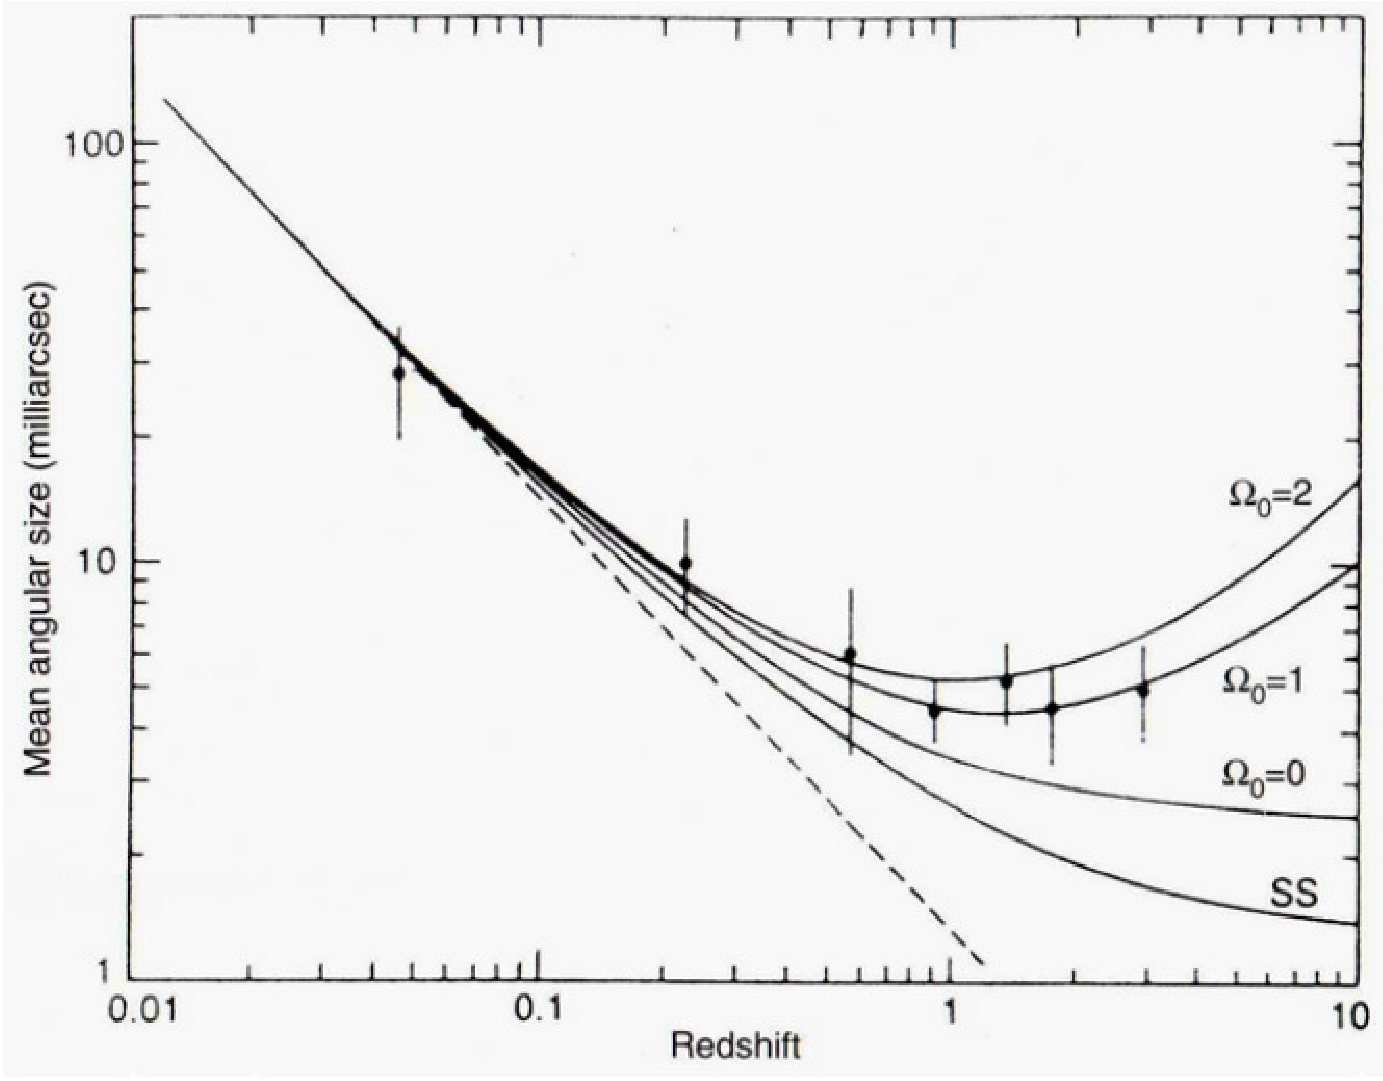
\includegraphics[width=0.8\textwidth]{figure/diametri_angolari_1.pdf}
  \caption{Diametro angolare apparente in funzione del logaritmo di $z$.  Al
    crescere di $q_0$ le curve mostrano un appiattimento a $z \simeq 1$ e quindi
    un aumento del diametro apparente a $z$ più alti}
  \label{diam_angolari_1}
\end{figure}
La lunghezza propria $D$ si calcola dalla metrica RW ponendo $dt=dr=d\phi=0$
\begin{equation}
  D= R(t_1) r_1 \Delta \theta  \implies \Delta \theta = \frac{D} {R(t_1) r_1}
\end{equation}
da cui segue
\begin{equation}
  d_A= R(t_1) r_1.
\end{equation}
Dalle definizioni di $d_L$ in \eqref{dis_lum} e $d_A$ segue
\begin{equation}
  d_A = d_L \left( \frac{R_1}{R_0} \right)^2 = \frac{d_L}{(1+z)^2}
\end{equation}
e quindi usando eq. \eqref{15324}
\begin{equation}
  d_A = \frac { \left[ z q_0 +(q_0-1) (-1+\sqrt{2q_0z+1}) \right] }  {H_0 q^2_0
    (1+z)^2}
  \iff
  \Delta \theta  = D \frac{H_0 q^2_0 (1+z)^2} {\left[ z q_0 +(q_0-1)
      (-1+\sqrt{2q_0z+1}) \right]}
\end{equation}
Qui anticipiamo alcune relazioni che troveremo nel capitolo successivo
\begin{align}
  \Omega_0 &= \frac{\rho_0 }{\rho_c}=2 q_0, \\
  \rho_c   &= \frac{3 H_0^2}{8 \pi G}
\end{align}
La fig.~\ref{diam_angolari_1} illustra l'andamento della dimensione angolare di
una sorgente in funzione di $z$ e la sua dipendenza da $q_0$.  Per $z\ll 1$
l'andamento è quello previsto in un universo Euclideo $\Delta \theta \propto
z^{-1}$ .  All'avvicinarsi a $z=1$ si verifica un appiattimento, e per valori di
$z>1$ una inversione per cui al crescere della distanza (e red-shift) la
dimensione apparente della sorgente cresce.  Tale comportamento, inaspettato in
un universo Euclideo, è dovuto al fatto che per distanze elevate cominciano ad
intervenire effetti di curvatura che modificano le traiettorie dei fotoni
rispetto alla propagazione rettilinea Euclidea.  Poiché la curvatura della
traiettoria di un fotone dipende (a parità di distanza) dalla densità media di
materia gravitante attraversata (che è misurata da $q_0$), vi sarà una
dipendenza di $\Delta \theta$ dai parametri di decelerazione e densità
$\Omega_0$ come mostrato nelle fig.~\ref{diam_angolari_1} \ref{diam_angolari_2}.
Possiamo vedere la cosa come un effetto di ``lente gravitazionale'' operata
dall'intero Universo e il cui effetto è di ingrandire le dimensioni apparenti di
oggetti lontanissimi.
\begin{figure}
  \centering{}
  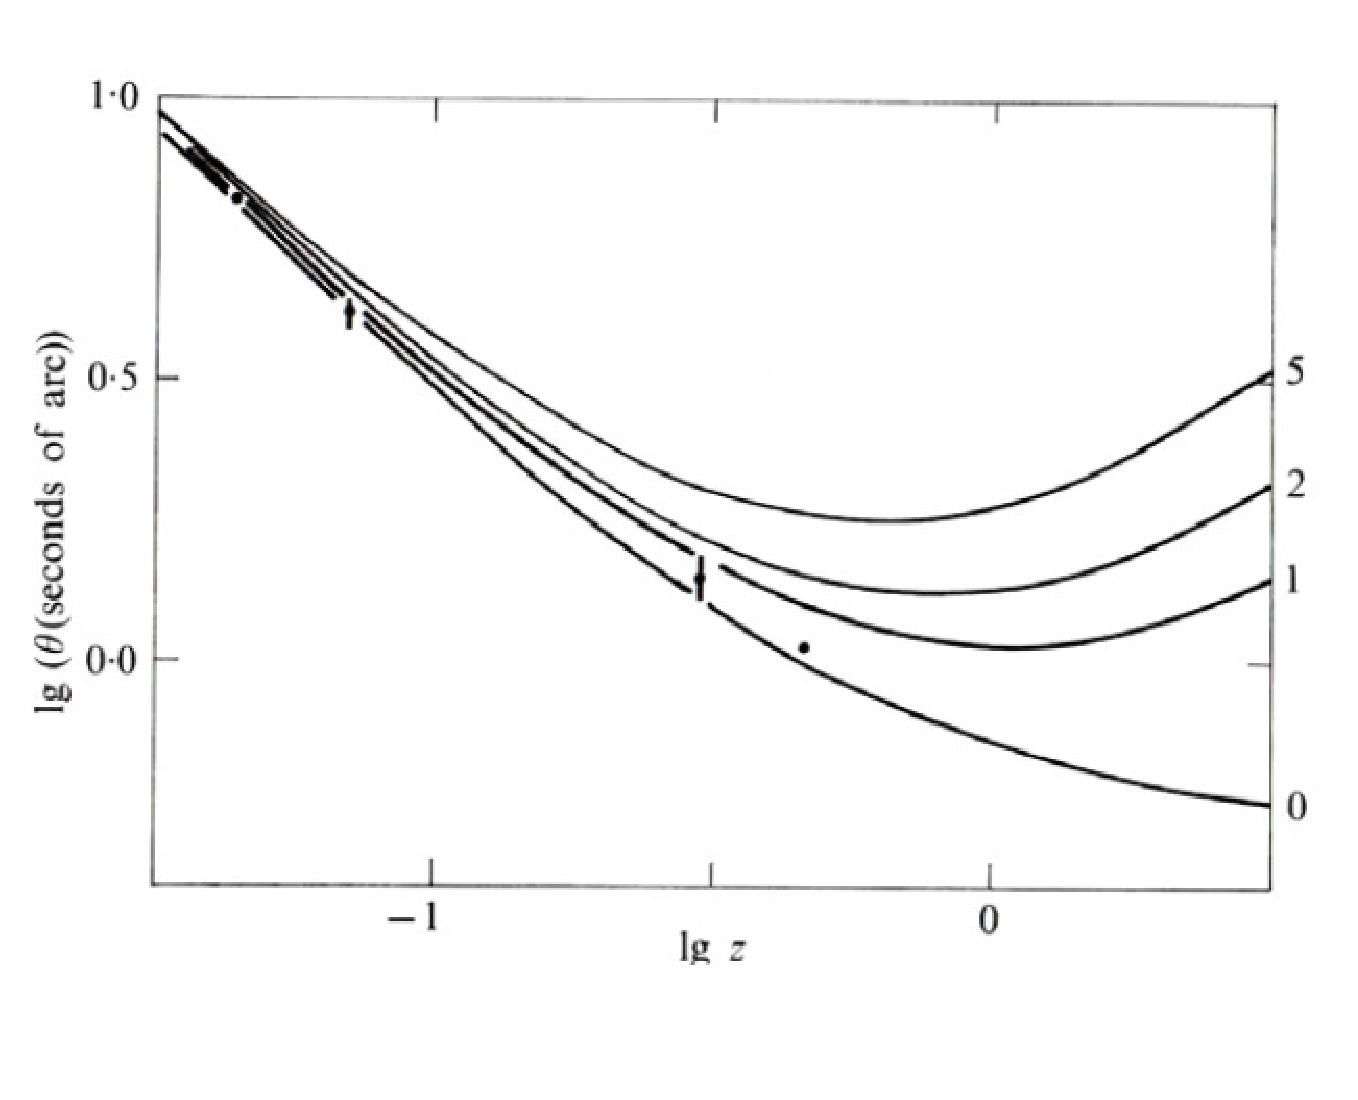
\includegraphics[width=0.75\textwidth]{figure/diametri_angolari_2.pdf}
  \caption{Diametro angolare e parametro di densità $\Omega_0$}
  \label{diam_angolari_2}
\end{figure}
L'utilizzo del test in riferimento alle dimensioni angolari delle radiosorgenti
compatte osservate con il sistema interferometrico ad altissima risoluzione VLBI
è consistente con $q_0=0.5$, come mostrato in fig.~\ref{diam_angolari_2}.

%%% Local Variables:
%%% mode: latex
%%% TeX-master: "../cosmo"
%%% fill-column: 80
%%% End:

\chapter{Cosmologia}
\label{cha:cosmologia}

\section{Equazioni di Einstein: Modello di Friedmann}

Si assume che la dinamica dell'Universo sia governata dalle eq. di Einstein, che
la metrica sia quella di RW e che il tensore energia-impulso sia quello di un
fluido perfetto.  La metrica dello spazio-tempo è
\begin{subequations}
  \label{rw1}
  \begin{align}
    g_{tt} &=-1, \\
    g_{it} &= 0, \\
    g_{ij} &= R^2(t) \tilde{g}_{ij}(x^i),
  \end{align}
\end{subequations}
dove $t$ è il tempo cosmico, $x^{i} = (r,\theta,\phi)$ sono coordinate sferiche
coomoventi e $\tilde{g}_{ij}(x^i)$ è la metrica su $^{3}$S
\begin{subequations}
  \label{rw2}
  \begin{align}
    \tilde{g}_{rr} &= (1-kr^2)^{-1}, \\
    \tilde{g}_{\theta \theta} &= r^2, \\
    \tilde{g}_{\phi \phi} &= r^2 \sin^2 \phi,
  \end{align}
\end{subequations}
tutti gli altri elementi della metrica sono nulli.

Il tensore energia-impulso ha la forma
\begin{equation}
  T_{\mu\nu} = p g_{\mu\nu} + (p+\rho) U_{\mu} U_{\nu}
  \label{fp}
\end{equation}
con $p$ pressione, $\rho$ densità di energia e $U^{\mu}=(1,0,0,0)$ 4-velocità
dei costituenti dell'Universo.

La dinamica dell'Universo è determinata dalle eq. di Einstein
\begin{equation}
  R_{\mu\nu} =-8\pi GS_{\mu \nu},
\end{equation}
con
\begin{equation}
  S_{\mu \nu}=T_{\mu \nu}-\frac{1}{2} g_{\mu \nu} \tensor{T}{^{\lambda}_{\lambda}}.
\end{equation}

Il tensore di Ricci diventa (il punto indica derivazione rispetto al tempo)
\begin{subequations}
  \begin{align}
    R_{tt} &= \frac{ 3 \ddot{R}}{R} \\
    R_{ti} &= 0 \\
    R_{ij} &= -(R\ddot{R}+2\dot{R}^2+2k) \tilde{g}_{ij}.
  \end{align}
\end{subequations}

Osserva che
\begin{equation}
  \tensor{T}{^{\lambda}}{_{\lambda}} = g^{\lambda\nu} T_{\lambda\nu} = p
  \tensor{\delta}{^{\lambda}}_{{\lambda}} + (p+\rho) (-1) = 3p - \rho
\end{equation}
così che il termine di sorgente diventa
\begin{equation}
  S_{\mu \nu} = \frac{1}{2} (\rho-p) g_{\mu\nu}+(p+\rho)U_{\mu} U_{\nu}
\end{equation}
In particolare
\begin{subequations}
  \begin{align}
    S_{tt} &= \frac{1}{2} (\rho-p)(-1)+(p+\rho)(+1) =
             \frac{1}{2} (\rho+3p) \\
    \label{sij}
    S_{ij} &= \frac{1}{2} (\rho-p) g_{ij}=
             \frac{1}{2} (\rho-p) R^2(t) \tilde{g}_{ij}
  \end{align}
\end{subequations}

Dalle eq. di Einstein per la componente $tt$ si ha:
\begin{equation}
  \frac{3 \ddot{R}}{R} = - 4\pi G (\rho+3p)
  \label{e1}
\end{equation}
e per la componente $ij$:
\begin{equation}
  \label{e2}
  \frac{\ddot{R}}{R} +\frac{2\dot{R}^2}{R^2}+\frac{2k}{R^2}= 4 \pi G (\rho-p)
\end{equation}
Si ha inoltre l'eq. di conservazione (da $\tensor{T}{^{\mu \nu}_{;\mu}}=0$, con $\nu =0$)
\begin{equation}
  \dot{p} R^3 = \toder{}{t}[R^3(\rho+p)]  \iff \toder{(\rho R^3)}{R} = -3pR^2
  \label{moto}
\end{equation}

Si osservi che le tre eq.  \eqref{e1}, \eqref{e2} e \eqref{moto} non sono
indipendenti (una può essere derivata dalle altre due).  Pertanto per risolvere
il problema cosmologico, cioè per determinare $R$, $\rho$ e $p$ in funzione del
tempo cosmico, è necessario introdurre un'ulteriore relazione.  Questa è
l'eq. di stato
\begin{equation}
  p=p(\rho)
  \label{stato}
\end{equation}
che ha i casi particolari $p=0$ per l'era della materia, $p=\rho/3$ per l'era
della radiazione.

Osserviamo infine che eliminando $\ddot{R}$ tra le eq.  \eqref{e1} e \eqref{e2},
si ottiene un'equazione differenziale del primo ordine, nota come
\emph{equazione di Friedmann}
\begin{equation}
  \dot{R}^2 +k = \frac{8 \pi G}{3} \rho R^2.
  \label{eq:friedmann}
\end{equation}

In conclusione, le eq. \eqref{eq:friedmann}, \eqref{moto} e \eqref{stato}
permettono di determinare le 3 funzioni incognite $R(t)$, $p(t)$ e $\rho(t)$.
Si otterranno 3 differenti soluzioni a seconda del valore di $k=-1,0,+1$.
Questi modelli cosmologici sono noti come modelli di Friedmann.

\textbf{Osservazione}: senza dare esplicitamente l'eq. di stato è possibile
ricavare informazioni sull'età $t_0$ dell'Universo e sull'andamento del fattore
di scala cosmico $R(t)$.  Infatti:
\begin{itemize}
\item $R(t)$ è una quantità definita positiva;
\item All'istante attuale $t_0$ l'Universo è in espansione ($\dot{R}_0 >0$)
  poichè noi oggi misuriamo red-shift ($z>0$);
\item L'eq. \eqref{e1} mostra che per materia ordinaria e radiazione $ \ddot{R}
  < 0$ sempre.  Quindi $R(t)$ ha concavità rivolta verso il basso ad ogni tempo,
  il che implica che per $t\rightarrow 0$, necessariamente $R \rightarrow 0$.
  Quindi i modelli di Friedmann prevedono l'esistenza di una singolarità
  iniziale.  Inoltre poichè $ \ddot{R} < 0$ sempre, $\dot{R}$ è una funzione
  decrescente e quindi la velocità di espansione dell'Universo $v_H(t) \propto
  \dot{R}$ diminuisce nel tempo, come ci si aspetta con gravità attrattiva.
\item Il termine a destra nell'eq. \eqref{eq:friedmann}, per $t>t_0$ ($t<t_0$)
  decresce (cresce) con il tempo --- rispetto al valore attuale --- almeno come
  $R^{-1}(t)$.
\end{itemize}

Da queste considerazioni segue che l'età dell'Universo è
\begin{equation}
  t_0 < H^{-1}_0  = \frac {R_0}{\dot{R}_0} = 13 \times 10^{9}
  \left(\frac{\SI[per-mode=reciprocal]{75}{\kilo\metre\per\second\per\mega\parsec}}{H_0}\right)
  \si{yr}.
\end{equation}
L'uguaglianza si avrebbe nel caso in cui fosse $\ddot{R} =0$, per cui $R(t)=t
\dot{R}$.  Per quanto riguarda il comportamento di $R(t)$ per $t>t_0$,
dall'eq. \eqref{eq:friedmann} si ha
\begin{itemize}
\item $R(t) \propto t$ nel caso $k=-1$, per il quale per $t \to \infty$,
  $\dot{R} \to 1$;
\item $R(t) \propto t^{2/3}$ nel caso $k=0$, per il quale per $t \to \infty$,
  $\dot{R} \propto R^{-1/2}$;
\item se $k=-1$, $\dot{R}$ decresce dal valore attuale (positivo) ed esisterà un
  istante $\tilde{t}$ a cui ${\dot R}=0$; a tempi successivi, il fattore di
  scala che ha concavità rivolta sempre verso il basso, continuerà a decrescere
  con il tempo fino ad un nuova singolarità.
\end{itemize}

\subsection{Derivazione newtoniana delle eq. di Friedmann}

Il teorema di Birkhoff afferma che un campo gravitazionale a simmetria sferica è
necessariamente statico ed è descritto dalla metrica di Schwarzschild.  Questo
risultato è l'analogo del risultato newtoniano (derivato dal teorema di Gauss)
che il campo all'esterno di una corpo a simmetria sferica è lo stesso che si
avrebbe se tutta la massa del corpo fosse concentrata al centro.  Il teorema di
Birkhoff può essere applicato anche al campo all'interno di una cavità sferica e
vuota che si trovi al centro di una distribuzione omogenea, non necessariamente
statica, di massa-energia.  In questo caso si prova che la metrica all'interno
della cavità è quella di Minkowski dello spazio piatto (cioè, il campo
gravitazionale è nullo all'interno).  L'analogo newtoniano di questa proprietà è
che il campo gravitazionale all'interno di una shell sferica e vuota è nullo.
Questo risultato è vero anche nel caso in cui la distribuzione di materia sia
infinita, l'unica condizione è che la distribuzione sia sfericamente simmetrica.

Consideriamo una cavità sferica di raggio $l$ al centro di una distribuzione
omogenea di massa.  All'interno la metrica è piatta e il campo gravitazionale è
nullo.  Si rimetta ora nella cavità una quantità di massa $m$, scelta in modo
tale che continui a valere la meccanica newtoniana, cioè
\begin{equation}
  \frac{Gm}{l c^2} \ll 1 \iff l \gg r_g(m).
  \label{41}
\end{equation}
La distanza $l$ nell'Universo in espansione è la distanza propria
\begin{equation}
  l(t) = R(t) r_0
\end{equation}
dove $r_0$ è una coordinata comovente che può essere scelta in modo che sia
valida la condizione in eq. \eqref{41}.  Applichiamo l'approssimazione
newtoniana per descrivere il moto di un punto P sulla sfera di raggio $l(t)$.
Si ha
\begin{equation}
  \toder[2]{l}{t} = -\frac{G m}{l^2} = \frac{4 \pi}{3} G \rho l
  \label{1103}
\end{equation}
o anche, moltiplicando per $\dot l$
\begin{equation}
  \frac{l}{2} \toder{\dot{l}^2}{t} = - \dot{l} \frac{G m}{l^2} = Gm  \toder{}{t}
  \left( \frac{1}{l} \right)
\end{equation}
e integrando
\begin{equation}
  \dot{l}^2 = \frac{2G m}{l} + \text{costante}.
  \label{219}
\end{equation}
Questa eq. rappresenta la conservazione dell'energia per unità di massa.
Utilizzando la relazione $l(t)=R(t) r_0$ si ha
\begin{equation}
  r_0^2 \dot{R}^2 = \frac{2Gm}{r_0 R} - k c^2 r_0^2
  \implies \dot{R}^2 = \frac{2G}{r_0^3 R} \frac{4 \pi \rho R^3 r_0^3}{3} - k c^2
\end{equation}
in cui abbiamo posto $\text{costante} = - k c^2 r_0^2$, con $k=-1$, $0$, $+1$, a
seconda del segno della costante.  Si ha quindi
\begin{equation}
  \dot{R}^2 + k c^2 = \frac{8 \pi}{3} G \rho R^2
  \label{1106}
\end{equation}
che è l'eq. di Friedmann \eqref{eq:friedmann}.  Il caso $k=1$ corrisponde a
$\text{costante}<0$ (energia totale negativa) e quindi il caso descrive la
situazione in cui un'eventuale espansione è seguita da collasso; il caso $k=-1$
corrisponde a $\text{costante}>0$ (energia totale positiva) e quindi espansione
continua per sempre.  Il caso $k=0$ corrisponde ad energia totale nulla e
rappresenta la situazione limite con velocità di espansione pari alla velocità
di fuga, per cui l'espansione cessa solamente per $t\to \infty$.

L'eq. \eqref{1106} è stata ottenuta assumendo che la sfera di raggio $l$
contenga solo materia non relativistica.  In Relatività Generale in presenza di
materia relativistica si ha che la densità di materia deve essere rimpiazzata da
(vedi eq. \eqref{e1})
\begin{equation}
  \rho \to  \rho + \frac{3 p}{c^2}
\end{equation}
dove $\rho$ è ora l'energia totale (energia associata alla massa a riposo +
energia interna).  In questo modo l'eq. \eqref{1103} diventa
\begin{equation}
  \ddot R = - \frac{4 \pi G }{3} \left( \rho + 3 \frac{p}{c^2} \right) R,
\end{equation}
che è l'analoga eq. \eqref{e1} ottenuta applicando la Relatività Generale.

Per quanto riguarda l'eq. di conservazione \eqref{moto}, essa si può ottenere
dalla I legge della termodinamica nel caso di espansione dell'Universo
adiabatica ($\dd Q=0$).  Si ha
\begin{equation}
  \dd U + p \dd V=0
\end{equation}
e sostituendo $U=\rho V c^2$, per cui $\dd U= V c^2 d\rho + \rho c^2 \dd V$, si
ha
\begin{equation}
  \rho \dd V + V \dd\rho = - \frac{p}{c^2} \dd V \implies
  \dd\rho= -\left( \rho + \frac{p}{c^2} \right) \frac{\dd V}{V}
\end{equation}
da cui segue
\begin{equation}
  \label{eq:continuita}
  d\rho= - \left( \rho + \frac{p}{c^2} \right) \frac{4 \pi l^2 dl}{4 \pi l^3/3}
  \implies \toder{\rho}{t} +  3 \left( \rho + \frac{p}{c^2} \right) \frac{\dot
    R }{R} =0
\end{equation}
che è equivalente all'eq. \eqref{moto}.

La densità critica $\rho_c$ si può ottenere ponendo in eq. \eqref{219}
$v=v_{c}$.  Si ha
\begin{equation}
  v^2_{c} = \frac{2 G m }{l}=\frac{2G}{l} \frac{4}{3} \pi \rho_c l^3 \implies
  \dot{R}^2= \frac{8 \pi G}{3} \rho_c R^2
\end{equation}
e per l'istante attuale $t_0$
\begin{equation}
\rho_c(t_{0}) = \frac{3 H_0^2}{8 \pi G}.
\end{equation}

\section{Densità e pressione dell'Universo presente}

All'istante attuale densità e pressione sono valutate dalle eq. dinamiche (con $t=t_0$)
\begin{subequations}
  \begin{align}
    \label{rho0}
    \rho_0  &= \frac{3}{8 \pi G} \left(\frac{k}{R_0^2} + H_0^2 \right) \\
    \label{p0}
    p_0 &= -\frac{1}{8 \pi G} \left[\frac {k}{R_0^2}+H_0^2(1-2q_0)\right].
  \end{align}
\end{subequations}
Se si definisce una \emph{densità critica}
\begin{equation}
  \rho_c \equiv  \frac{3 H_0^2}{8 \pi G} = 1.1 \times 10^{-29}
  \left(
    \frac{H_0}{\SI[per-mode=reciprocal]{75}{\kilo\metre \per \second \per
        \mega\parsec}}
  \right)^2
  \si{\gram\per\centi\metre\cubed}
  \label{rhoc}
\end{equation}
l'eq. \eqref{rho0} diventa
\begin{equation}
  \rho_0-\rho_c =  \frac{3 k}{8 \pi G R_0^2},
  \label{temp1}
\end{equation}
per cui l'Universo ha curvatura spaziale positiva o negativa a seconda che sia
$\rho_0 > \rho_c$ oppure $\rho_0 < \rho_c$.

Possiamo mettere in relazione $\rho_0$ e $\rho_c$ con il parametro di
decelerazione $q_0$.  Infatti per l'Universo presente che è dominato dalla
materia, si ha $p_0=0$, così che dall'equazione~\eqref{p0} segue
\begin{equation}
  \frac{k}{R_0^2} = H_0^2 (2q_0-1)
\end{equation}.
Sostituendo nella \eqref{temp1} si ottiene infine
\begin{equation}
  \frac{\rho_0}{\rho_c}=2 q_0
  \label{rho0surhoc}
\end{equation}
pertanto
\begin{itemize}
\item se $q_0 > 1/2 \implies \rho_0>\rho_c$, $k=+1$
\item se $q_0 = 1/2 \implies \rho_0=\rho_c$, $k=0$
\item se $q_0 < 1/2 \implies \rho_0<\rho_c$, $k=-1$
\end{itemize}

Poiché oggi $\rho_*(0) \ll \rho_c$ e inoltre la radiazione di fondo cosmico non
contribuisce in maniera apprezzabile a $\rho_0$, se $q_0 \ge 0.5$ esisterà
nell'Universo DM.  La densità di energia mancante non potrà comunque essere in
forma di barioni (diffusi sotto forma di idrogeno neutro e/o molecolare) poiché
per la Nucleosintesi (come si vedrà) $\rho_B < 0.05 \rho_c$.

\section{Era dominata dalla materia}

All'istante attuale l'Universo è nell'era della materia, e questa si estende
indietro nel tempo fino a valori di red-shift $z \simeq 1000$.  Infatti dalla
relazione
\begin{equation}
  \frac {\rho_m(t)} {\rho_r(t)} \simeq  10^{3} \frac {R(t)} {R_0} \equiv  10^3
  \frac{1}{1+z}
\end{equation}
si ha che l'Universo entra nell'era della radiazione ($\rho_m = \rho_r$) quando
$z = 1000$.  Questo accade (come vedremo) ad un tempo $ \simeq 10^5$ yr (a
partire dalla singolarità iniziale).  Tale valore è trascurabile rispetto al
tempo attuale dell'Universo $t_0 \simeq 14 \times 10^9$ yr e pertanto porremo
l'inizio di tale era a $t=0$.  Riprendiamo in esame l'eq. di Friedmann
\eqref{eq:friedmann} in cui poniamo
\begin{equation}
  \rho = \rho_0 \left( \frac {R_0} {R} \right)^{3}
\end{equation}
È conveniente esprimere $\rho_0$ e $k/R^2$ in termini di $q_0$ ed $H_0$.
Dall'eq. \eqref{p0} segue
\begin{equation}
  \frac{k}{R_0^2}=(2q_0-1) H_0^2~,
\end{equation}
e sostituendo nell'eq. \eqref{rho0} si ha
\begin{equation}
  \frac{8\pi G}{3} \rho_0 = 2q_0 H_0^2
\end{equation}
Usando le relazioni precedenti l'eq. \eqref{eq:friedmann} diventa:
\begin{equation}
  \dot{R}^2 + (2 q_0-1) H_0^2 R_0^2 = \frac{8\pi G}{3} \rho_0 \frac{R_0^3}{R},
\end{equation}
o, equivalentemente,
\begin{equation}
  \left(\frac{\dot R}{R_0}\right)^2 = H_0^2 \left(1-2q_0+2 q_0
    \frac{R_0}{R}\right)
\end{equation}
Con la posizione $x=R(t)/R_0$ si ha infine
\begin{equation}
  \toder{x}{t}= H_0 \left(1-2q_0+ \frac {2q_0}{x}\right)^{1/2},
  \label{2.40}
\end{equation}
la cui soluzione formale è
\begin{equation}
  t= H_0^{-1} \int_0^{R/R_0} dx \left(1-2q_0+\frac{2q_0}{x}\right)^{-1/2}
  \label{efa}
\end{equation}
L'età dell'Universo è ottenuta integrando sino a $x=1$
\begin{equation}
  t_0= H_0^{-1} \int_0^{1} dx \left(1-2q_0+\frac{2q_0}{x}\right)^{-1/2}
\end{equation}
e quindi risulta $t_0< H_0^{-1}$.  L'eq. \eqref{efa} può essere risolta
analiticamente nei tre casi $k=+1$, $0$, $-1$.

\subsubsection{Caso A: $q_0 > 1/2$, $k=+1$, $\rho_0> \rho_c$}

Definiamo l'angolo $\theta$ attraverso la relazione:
\begin{equation}
  1-\cos \theta = \left(\frac{2q_0-1 }{q_0}\right) x \qquad\text{con}\qquad x=0
  \iff \cos \theta=1
  \label{posizioneiniziale}
\end{equation}
da cui segue
\begin{equation}
  \dd x =   \left(\frac{- q_0}{2q_0-1}\right)  \dd \cos \theta
\end{equation}
Con questa posizione l'integrale in eq. (\ref{efa}) diventa:
\begin{equation}
  \begin{split}
    t H_0 &= \int _1^{\cos \theta} \left[1-2q_0+2q_0 \left(\frac{2q_0-1}{q_0}
      \right) \left(\frac{1}{1-\cos \theta} \right) \right]^{-1/2} \dd\cos\theta
    \left(\frac{-q_0}{2q_0-1} \right) \\
    &=\left( \frac{-q_0}{2q_0-1} \right) \int _1^{\cos \theta} \left[
      \frac{1-\cos \theta - 2q_0 + 2q_0 \cos \theta + 4q_0 -2} {1-\cos\theta}
    \right]^{-1/2} \dd\cos\theta \\
    &=\left( \frac {-q_0}{2q_0-1} \right) \int _1^{\cos \theta} \left[ \frac
      {1-\cos \theta} {\cos \theta (2q_0-1) + (2q_0-1)} \right]^{1/2}
    \dd\cos\theta \\
    &= \left( \frac {-q_0}{(2q_0-1)^{3/2}} \right) \int_1^{\cos \theta} \sqrt
    \frac{1-\cos \theta}{1+\cos \theta} \dd \cos \theta
  \end{split}
\end{equation}
Osserva che
\begin{equation}
  \int \sqrt \frac {1-y}{1+y} \dd y = \sqrt {1-y} + \arcsin y.
\end{equation}
Allora si ha
\begin{equation}
  \begin{split}
    t & = \left( \frac {-q_0}{H_0 (2q_0-1)^{3/2}} \right)
    \left[ \sqrt {1-\cos\theta^2} + \arcsin \cos \theta - \arcsin 1 \right] \\
    & = \left( \frac {-q_0}{H_0(2q_0-1)^{3/2}} \right) \left[ \sin \theta +
      {\pi}/{2} - \theta - {\pi}/{2}\right] \\
    & = \left( \frac {-q_0}{H_0(2q_0-1)^{3/2}} \right) \left[ \theta - \sin \theta
    \right].
    \label{sema}
  \end{split}
\end{equation}
(Nella derivazione precedente, applico $\cos \theta = \sin (\pi/2-\theta)$ e
$\arcsin \sin \theta = \theta$.)

Questa relazione insieme alla posizione iniziale \eqref{posizioneiniziale}
\begin{equation}
  R(t)= \left( \frac {R_0 q_0} {2q_0-1} \right) (1-\cos \theta)
\end{equation}
mostra che $R(t)$ si comporta come una cicloide ($R(t$ sia la coordinata di un
punto sulla superficie di un disco che avanza rotolando e senza strisciare): a
partire dal tempo $t=0$ ($\theta=0$) a cui $R(0)=0$, $R(t)$ aumenta fino ad un
valore massimo $R_{max}= {2 q_0 R_0 }/({2q_0-1})$ che si verifica al tempo
$t_{max}= \pi q_0/(2q_0-1)^{3/2}$.  A tempi successivi $R(t)$ decresce e ritorna
a zero quando $t=2t_{max}$ ($\theta =2 \pi$).

L'istante attuale è ottenuto ponendo $R(t)=R_0$
\begin{subequations}
  \begin{align}
    \cos\theta_0 &= \frac {1} {q_0} -1 \\
    t_0 &= \frac {q_0}{H_0 (2q_0-1)^{3/2}} \left(\arccos(\frac {1}{q_0}-1) -
          \frac {1}{q_0}(2q_0-1)^{1/2} \right)
  \end{align}
\end{subequations}
(Nella derivazione, applico $\sin \theta_0= \sqrt{1-\cos^2\theta_0}=
{q_0^{-1}\sqrt{2q_0-1}}$).

Se poniamo $q_0=1$ (cioè $\cos \theta_0=0$), allora avremo $t_0 = H_0^{-1} (\pi
/2-1) = 7.5$ miliardi di anni e $t_{max} = 40$ miliardi di anni.  L'intero ciclo
si compierebbe in $80$ miliardi di anni.  Qui abbiamo usato i valori $H_0^{-1} =
13$ miliardi di anni, corrispondente ad
$H_0 = 75$ km/s/Mpc.

\subsubsection{Caso B: $q_0 = 1/2$, $k=0$, $\rho_0= \rho_c$}

Questo caso è noto come Universo di Einstein-de Sitter.  L'eq. \eqref{efa}
diventa
\begin{equation}
  t = H_0^{-1} \int_0^{R/R_0} \sqrt x dx = H_0^{-1} \frac{2} {3} x^{3/2}
\end{equation}
da cui segue
\begin{equation}
  \frac{R(t)}{R_0} = \left( \frac {3H_0 t}{2} \right)^{2/3}.
\end{equation}
Il fattore di scala cosmico $R(t)$ aumenta senza limiti; l'istante attuale è
$t_0=2H_0^{-1}/3$ e risulta pari a $t_0= 9$ miliardi di anni ($H_0= 75$
km/s/Mpc).

\subsubsection{Caso C: $0< q_0 < 1/2$, $k=-1$, $\rho_0 < \rho_c$}

Con la posizione $\theta = i \phi$ si ottengono risultati analoghi al caso A.
In particolare:
\begin{gather}
  t H_0= \frac {q_0}{(-2q_0+1)^{3/2}} \left( \sinh \phi \ - \phi \right)
  \label{topen} \\
  \cosh \phi -1 = \left( \frac {1-2q_0}{q_0} \right) \frac {R(t)}{R_0}
  \label{cosht}
\end{gather}
Per $t \to \infty$ si ha
\begin{equation}
  \frac{R(t)}{R_0} \simeq \frac {q_0}{2(1-2q_0)} e^{\phi} \simeq \sqrt{1-2q_0}
  H_0 t
\end{equation}
L'istante attuale è ottenuto ponendo $R(t_0)= R_0$ nell'eq. \eqref{cosht}.  Si
ha così $\cosh \phi_0= q_0^{-1}-1$, e sostituendo nella eq. \eqref{topen} si ha
infine
\begin{equation}
  \begin{split}
    t_0 &= \left(\frac {q_0}{H_0 (1-2q_0)^{3/2}} \right)
    \left[- \cosh^{-1} (q_0^{-1}-1) + \sqrt{1+(q_0^{-1}-1)^2} \right] \\
    &= H_0^{-1} \left[ (1-2q_0)^{-1} - q_0 (1-2q_0)^{-3/2} \cosh^{-1}
      (q_0^{-1}-1) \right]
  \end{split}
\end{equation}
Ad esempio se assumiamo $\rho_0 =\rho_*$ (non ci sia DM e tutti i barioni
presenti nell'Universo siano nelle stelle) si ottiene $q_0 = 0.014$ e quindi
$t_0 \simeq 0.96 H_0^{-1} \simeq 13$ miliardi di anni.

Osserviamo che dallo studio delle abbondanze degli isotopi degli elementi
radioattivi si può determinare l'età della Terra $\simeq $ 4.5 miliardi di anni
e della Galassia $\simeq 7$ miliardi di anni.  Comunque gli oggetti più vecchi
nell'Universo sono gli ammassi globulari la cui età $\simeq 14$ miliardi di
anni.

\section{Eq. di Einstein e Costante Cosmologica/Dark Energy}

Prima della scoperta (Hubble 1929) dell'espansione dell'Universo, Einstein ha
modificato le eq. di campo introducendo un termine con costante cosmologica
$\Lambda$, perchè in questo modo le eq. prevedono una soluzione stazionaria con
$R$, $\rho$ e $p$ costanti nel tempo. L'eq. di campo modificate sono
\begin{equation}
  R_{\mu \nu} - \frac{1}{2} g_{\mu \nu} R - \Lambda g_{\mu \nu} =
  - 8 \pi G T_{\mu \nu}
  \label{EECC1}
\end{equation}
Moltiplicando per $g^{\mu \nu}$ si ha $R - (1/2) 4 R - 4\Lambda = -8 \pi G
\tensor{T}{^{\lambda}_{\lambda}}$, cioè $R=8 \pi G
\tensor{T}{^{\lambda}_{\lambda}} - 4 \Lambda$.  Sostituendo l'espressione di $R$
trovata e portando a destra i termini $R g_{\mu \nu}/2$ e $\Lambda g_{\mu \nu}$,
si ha la forma equivalente
\begin{equation}
  R_{\mu \nu} = - 8 \pi G   \left(
    T_{\mu \nu} - \frac {1}{2} g_{\mu \nu} \tensor{T}{^{\lambda}_{\lambda}} +
    \rho_{\Lambda} g_{\mu \nu} \right) \qquad\text{con}\qquad \rho_{\Lambda} =
  \frac {\Lambda c^2} {8 \pi G}
  \label{EECC2}
\end{equation}
Compare quindi un termine di sorgente
\begin{equation}
  S_{\mu \nu}=T_{\mu \nu} - \frac {1}{2} g_{\mu \nu}
  \tensor{T}{^{\lambda}_{\lambda}} + \rho_{\Lambda}
\end{equation}
che include la densità $\rho_{\Lambda}$.  Nel caso $\mu=\nu=0$ si ha
\begin{equation}
  S_{tt} = \frac {1}{2} (\rho+3p) - \rho_{\Lambda},
  \label{945}
\end{equation}
e pertanto, poiché in analogia al caso di materia ordinaria il termine di
sorgente atteso per la costante cosmologica è $(\rho_{\Lambda}+3p_{\Lambda})/2$
e invece abbiamo il termine $-\rho_{\Lambda}$, l'eq. stato sottostante è
$p_{\Lambda} = - \rho_{\Lambda}$.  Osserviamo che questo è un caso particolare
di una più generale eq. di stato per la componente Dark Energy (DE)
\begin{equation}
  p_{DE}= w \rho_{DE} \qquad\text{con } w<0
\end{equation}

Prima di procedere, osserviano che se il termine con costante cosmologica è
sempre dominante per cui $\rho \simeq \rho_{\Lambda}$ e $p \simeq p_{\Lambda}$,
le eq. del moto \eqref{moto} danno la soluzione stazionaria con $\rho (t) \simeq
\text{costante}$ (Universo stazionario).

Vediamo ora come le eq. \eqref{e1}, \eqref{e2} e \eqref{eq:friedmann} sono
modificate per l'introduzione di $\rho_{\Lambda}$ e $p_{\Lambda}$.  Uguagliando
$S_{tt}$ alla componente $R_{tt}= 3 \ddot{R}/R$, in sostituzione
dell'eq. \eqref{e1}, si ha ora:
\begin{equation}
  \frac{3 \ddot{R}}{R} = - 8\pi G \left[ \frac{1}{2}  (\rho+3p) - \rho_{\Lambda}
  \right]
  \label{ecc1}
\end{equation}
e, in termini della densità critica $\rho_c(0)=3H_0^2/(8\pi G)$
\begin{equation}
  \frac {\ddot{R}} {R} = - \frac {H_0^2} {\rho_c(0)}
  \left[
    \frac {1}{2}  (\rho+3p) - \rho_{\Lambda}
  \right]
\label{2.63}
\end{equation}
ed infine ponendo per le componenti ordinarie (materia e radiazione)
$\rho=\rho_m+\rho_r$, $p=p_m+p_r$, per l'era della materia $\rho
\simeq \rho_m$ e $p_m=0$ segue
\begin{equation}
  \label{ddRcc}
  \frac {\ddot{R}} {R} = H_0^2
  \left[ \Omega_{\Lambda} -\frac{\Omega_m (1+z)^3}{2} \right]
\end{equation}
con
\begin{subequations}
  \begin{align}
    \Omega_{\Lambda} &= \frac{\rho_{\Lambda}}{\rho_c(0)}, \\
    \Omega_m       &= \frac{\rho_m(0)}{\rho_c(0)}.
  \end{align}
\end{subequations}
Nella relazione precedente si pone anche $\rho_m(t)=\rho_m(0) [R_0/R(t)]^3 = \rho_m(0) (1+z)^3$.

In maniera analoga il termine $S_{ij}$ diventa
\begin{equation}
  S_{ij}= \left[ \frac {1}{2}(\rho-p)  + \rho_{\Lambda} \right] R^2(t)
  \tilde{g}_{ij}
  \label{sijcc}
\end{equation}
e l'q. \eqref{e2}  è ora sostituita da
\begin{equation}
  \frac {\ddot{R}}{R}+\frac{2\dot{R}^2}{R^2}+\frac{2k}{R^2}=
  8 \pi G \left[ \frac{1}{2}(\rho-p) +\rho_{\Lambda} \right]
\end{equation}
Eliminando $\ddot R$, con l'uso dell'eq. (\ref{ecc1}), si ha
\begin{equation}
  \frac{\dot{R}^2}{R^2} +\frac{k}{R^2} = \frac{8 \pi G}{3} (\rho+\rho_{\Lambda}).
\label{2.67}
\end{equation}
Questa relazione sostituisce l'eq. di Friedmann~\eqref{eq:friedmann}.  Per l'era
della materia l'equazione~\eqref{2.67} diventa
\begin{equation}
  H(z)=H_0\left[\Omega_{\Lambda}+\Omega_{k}(1+z)^2+\Omega_m (1+z)^3\right]^{1/2}
  \label{hzcc}
\end{equation}
dove ora
\begin{equation}
  \Omega_k = - \frac {k}{R_0^2 H_0^2}
\end{equation}
L'eq. \ref{hzcc} riferita all'istante attuale $z=0$ diventa
\begin{equation}
  \Omega_{\Lambda}+\Omega_{k}+\Omega_m = 1
\end{equation}
Per il parametro di decelerazione, da eq.(\ref{2.63}) con $z=0$, si ha invece:
\begin{equation}
  q_0 \equiv  -\frac {\ddot R_0 R_0}{\dot R^2_0} = \frac{\Omega_m}{2}
  -\Omega_{\Lambda}.
  \label{q0cc}
\end{equation}
In particolare, se $\Omega_{\Lambda} > \Omega_m/2$, allora $q_0<0$ e
$\ddot{R}_0>0$ e quindi $\dot{R}_0$ crescente, cioè l'Universo sarebbe oggi in
una fase di espansione accelerata.  Osserviamo infine che se $k=0$, allora
$\Omega_{\Lambda} + \Omega_m = 1$.
\begin{figure}
  \centering{}
  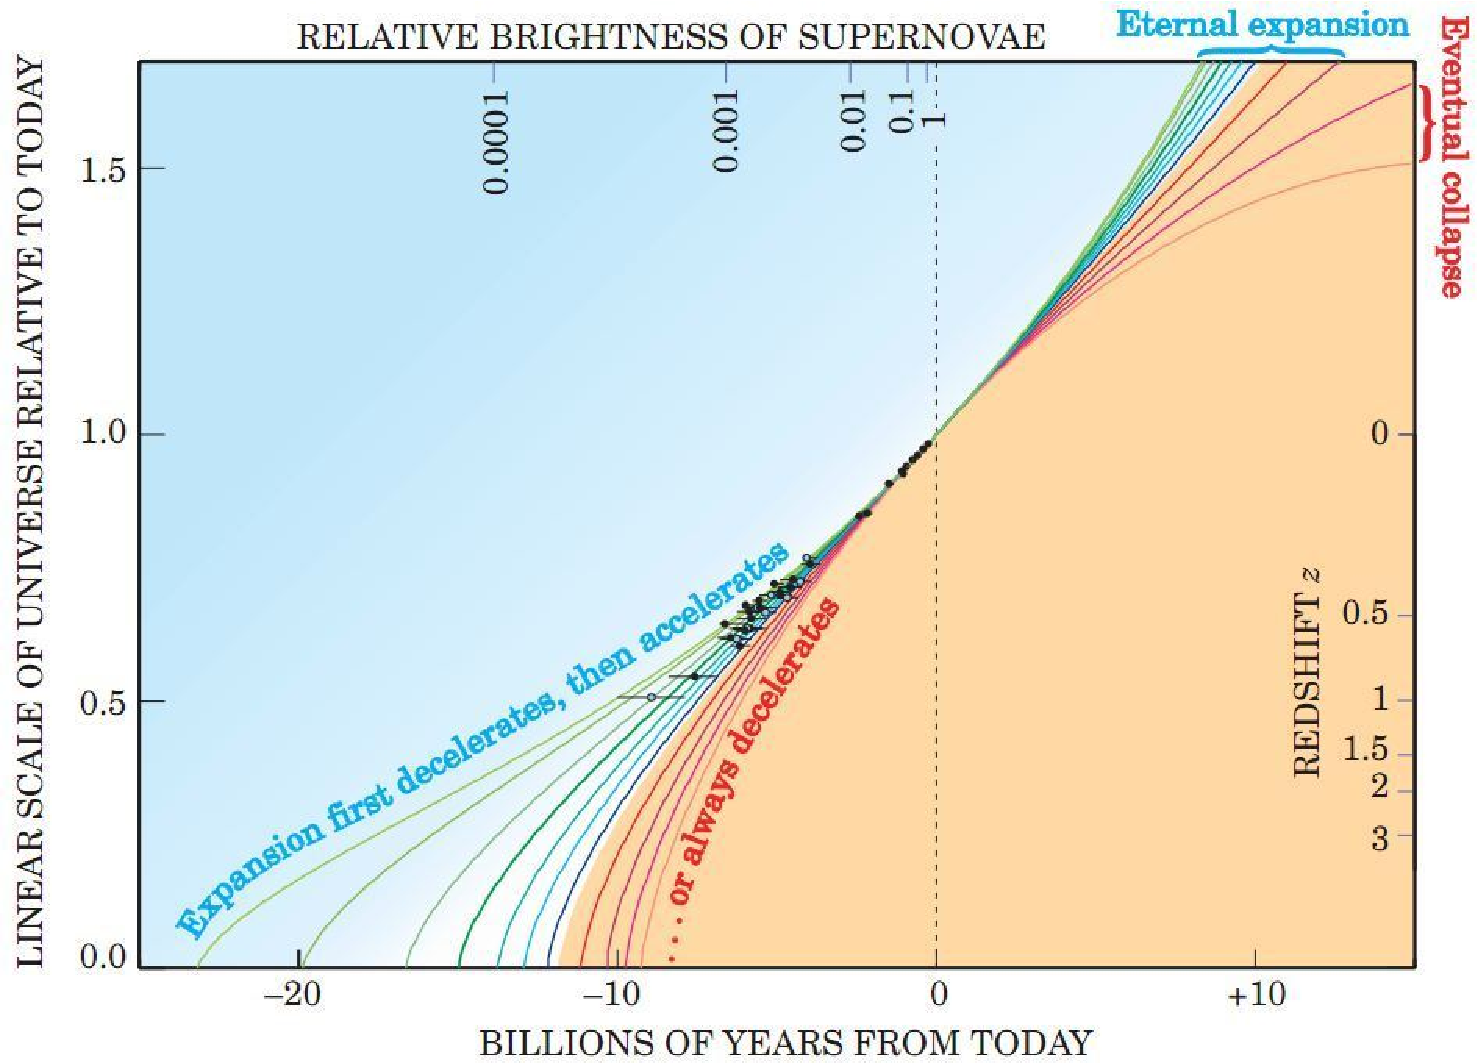
\includegraphics[width=0.8\textwidth]{figure/Scale_Factor_vs-Time.pdf}
  \caption{Andamento $R=R(t)$}
  \label{fig:Rvst}
\end{figure}

Vediamo come sia possibile determinare i parametri di densità $\Omega_i$
attraverso misure di distanza e red-shift.  In effetti, il modo in cui la
costante di Hubble $H(z)$ dipende da $z$ influenza la relazione tra magnitudine
e red-shift.  Preliminarmente osserviamo che dalla definizione $z=R_0/R(t) -1$,
segue
\begin{equation}
  \dd z = -\frac {R_0}{R(t)} H(t) \dd t.
\end{equation}
Consideriamo ora segnali luminosi (per i quali è $d \tau=0$) emessi al tempo $t$
da una galassia che abbia coordinata radiale $r$, e che raggiungono noi (che siamo in
$r=0$) all'istante $t_0$.  Dalla metrica RW si ha
\begin{equation}
  \int_t^{t_0} \frac {\dd t}{R(t)}= \int_0^{r} \frac {\dd r}{\sqrt{1-kr^2}}
  \simeq r + \mathcal{O}(r^3),
\end{equation}
Si ha quindi
\begin{equation}
  r \simeq \int_0^z \frac{\dd z}{R_0 ~ H(t)}.
\end{equation}
La distanza di luminosità $d_L = r R_0 (1+z)$ diventa allora
\begin{equation}
  \begin{split}
    d_L(z) & = (1+z) \int_0^z \frac{\dd z}{H(z)} = \\
           & = (1+z) \int_0^z \frac{\dd z}{H_0
             \left[\Omega_{\Lambda}+\Omega_{k}(1+z)^2+\Omega_m
               (1+z)^3\right]^{1/2}}.
  \end{split}
\end{equation}
Quindi a parità di $z$, gli oggetti osservati (di stessa magnitudine assoluta
$M$) appaiono più o meno lontani a seconda del valore dei parametri cosmologici
(vedere Fig. \ref{fig:Par_Cosm} dove per le supernovae \footnote{In sistemi
  binari di una nana bianca ed una gigante rossa, la massa espulsa dalla gigante
  rossa cade sulla nana bianca, che esplode in supernova quando la sua massa
  supera la massa limite di Chandrasekar. Si ritiene che queste supernovae
  abbiano la stessa luminosità intrinsceca, indipendentemente dalla distanza.}
di tipo Ia (??per la presenza o assenza di particolari righe??) è mostrata la
distanza $d_L$ in funzione del red-shift $z$).  È evidente allora che lo studio
del diagramma $m-z$ per questi oggetti (sufficientemente lontani) permette di
determinare i valori dei parametri $\Omega_{\Lambda}$, $\Omega_{k}$ ed
$\Omega_{m}$.
% In particolare si ha $\Omega_m = 0.27$ ed $\Omega_{\Lambda} =0.73$, se si
% assume $\Omeka_k=0$, il che è dedotto dall'analisi delle anisotropie della
% temperatura della CMB.%


Ricordiamo che per i modelli di Friedmann, la relazione $d_L=d_L(z)$ era
\begin{equation}
  d_L = \frac {1}{H_0} \left[ z+ \frac{1}{2}(1-q_0)z^2\right].
\end{equation}

Questo programma è stato realizzato prendendo come indicatori di distanza le
supernovae di tipo Ia~\parencites{1998AJ....116.1009R}{1999ApJ...517..565P}
\begin{figure}
  \centering
  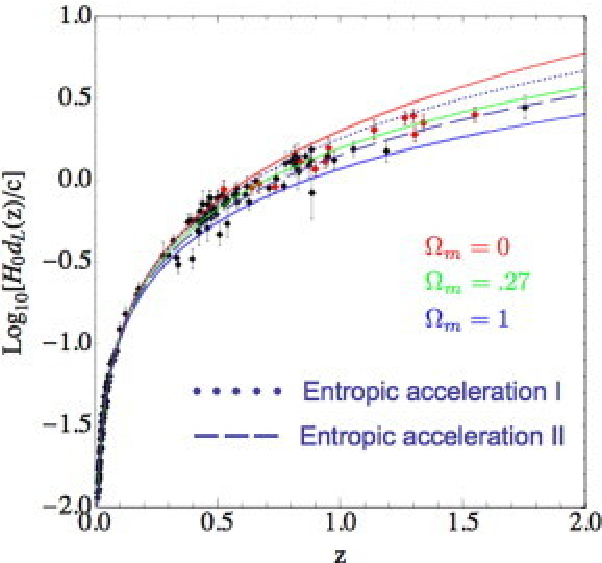
\includegraphics[width=0.8\textwidth]{figure/Hubble_Diagr_1_SNIa.pdf}
  \caption{Diagramma di Hubble SNIa}
  \label{fig:DHSN1}
\end{figure}
% \begin{figure}
%   \centering
%   \includegraphics[scale=1.2]{figure/Hubble_Diagr_2_SNIa.pdf}
%   \caption{Diagramma di Hubble SNIa.}
%   \label{fig:DHSN2}
% \end{figure}
e unitamente all'analisi di dati relativi all'anistrotropia della temperatura
della CMB e della funzione di correlazione angolare di galassie, si sono
determinati i seguenti valori
\begin{subequations}
  \begin{align}
    \Omega_k &= 0, \\
    \Omega_{\Lambda} &\simeq 0.7, \\
    \Omega_{m} &\simeq 0.3.
  \end{align}
\end{subequations}
La figura~\ref{fig:Par_Cosm} mostra che nello spazio dei parametri cosmologici
vi sono tre differenti regioni permesse --- quelle che danno $\chi^2<1$ --- la
cui intersezione determina la regione di valori permessi.
\begin{figure}
  \centering{}
  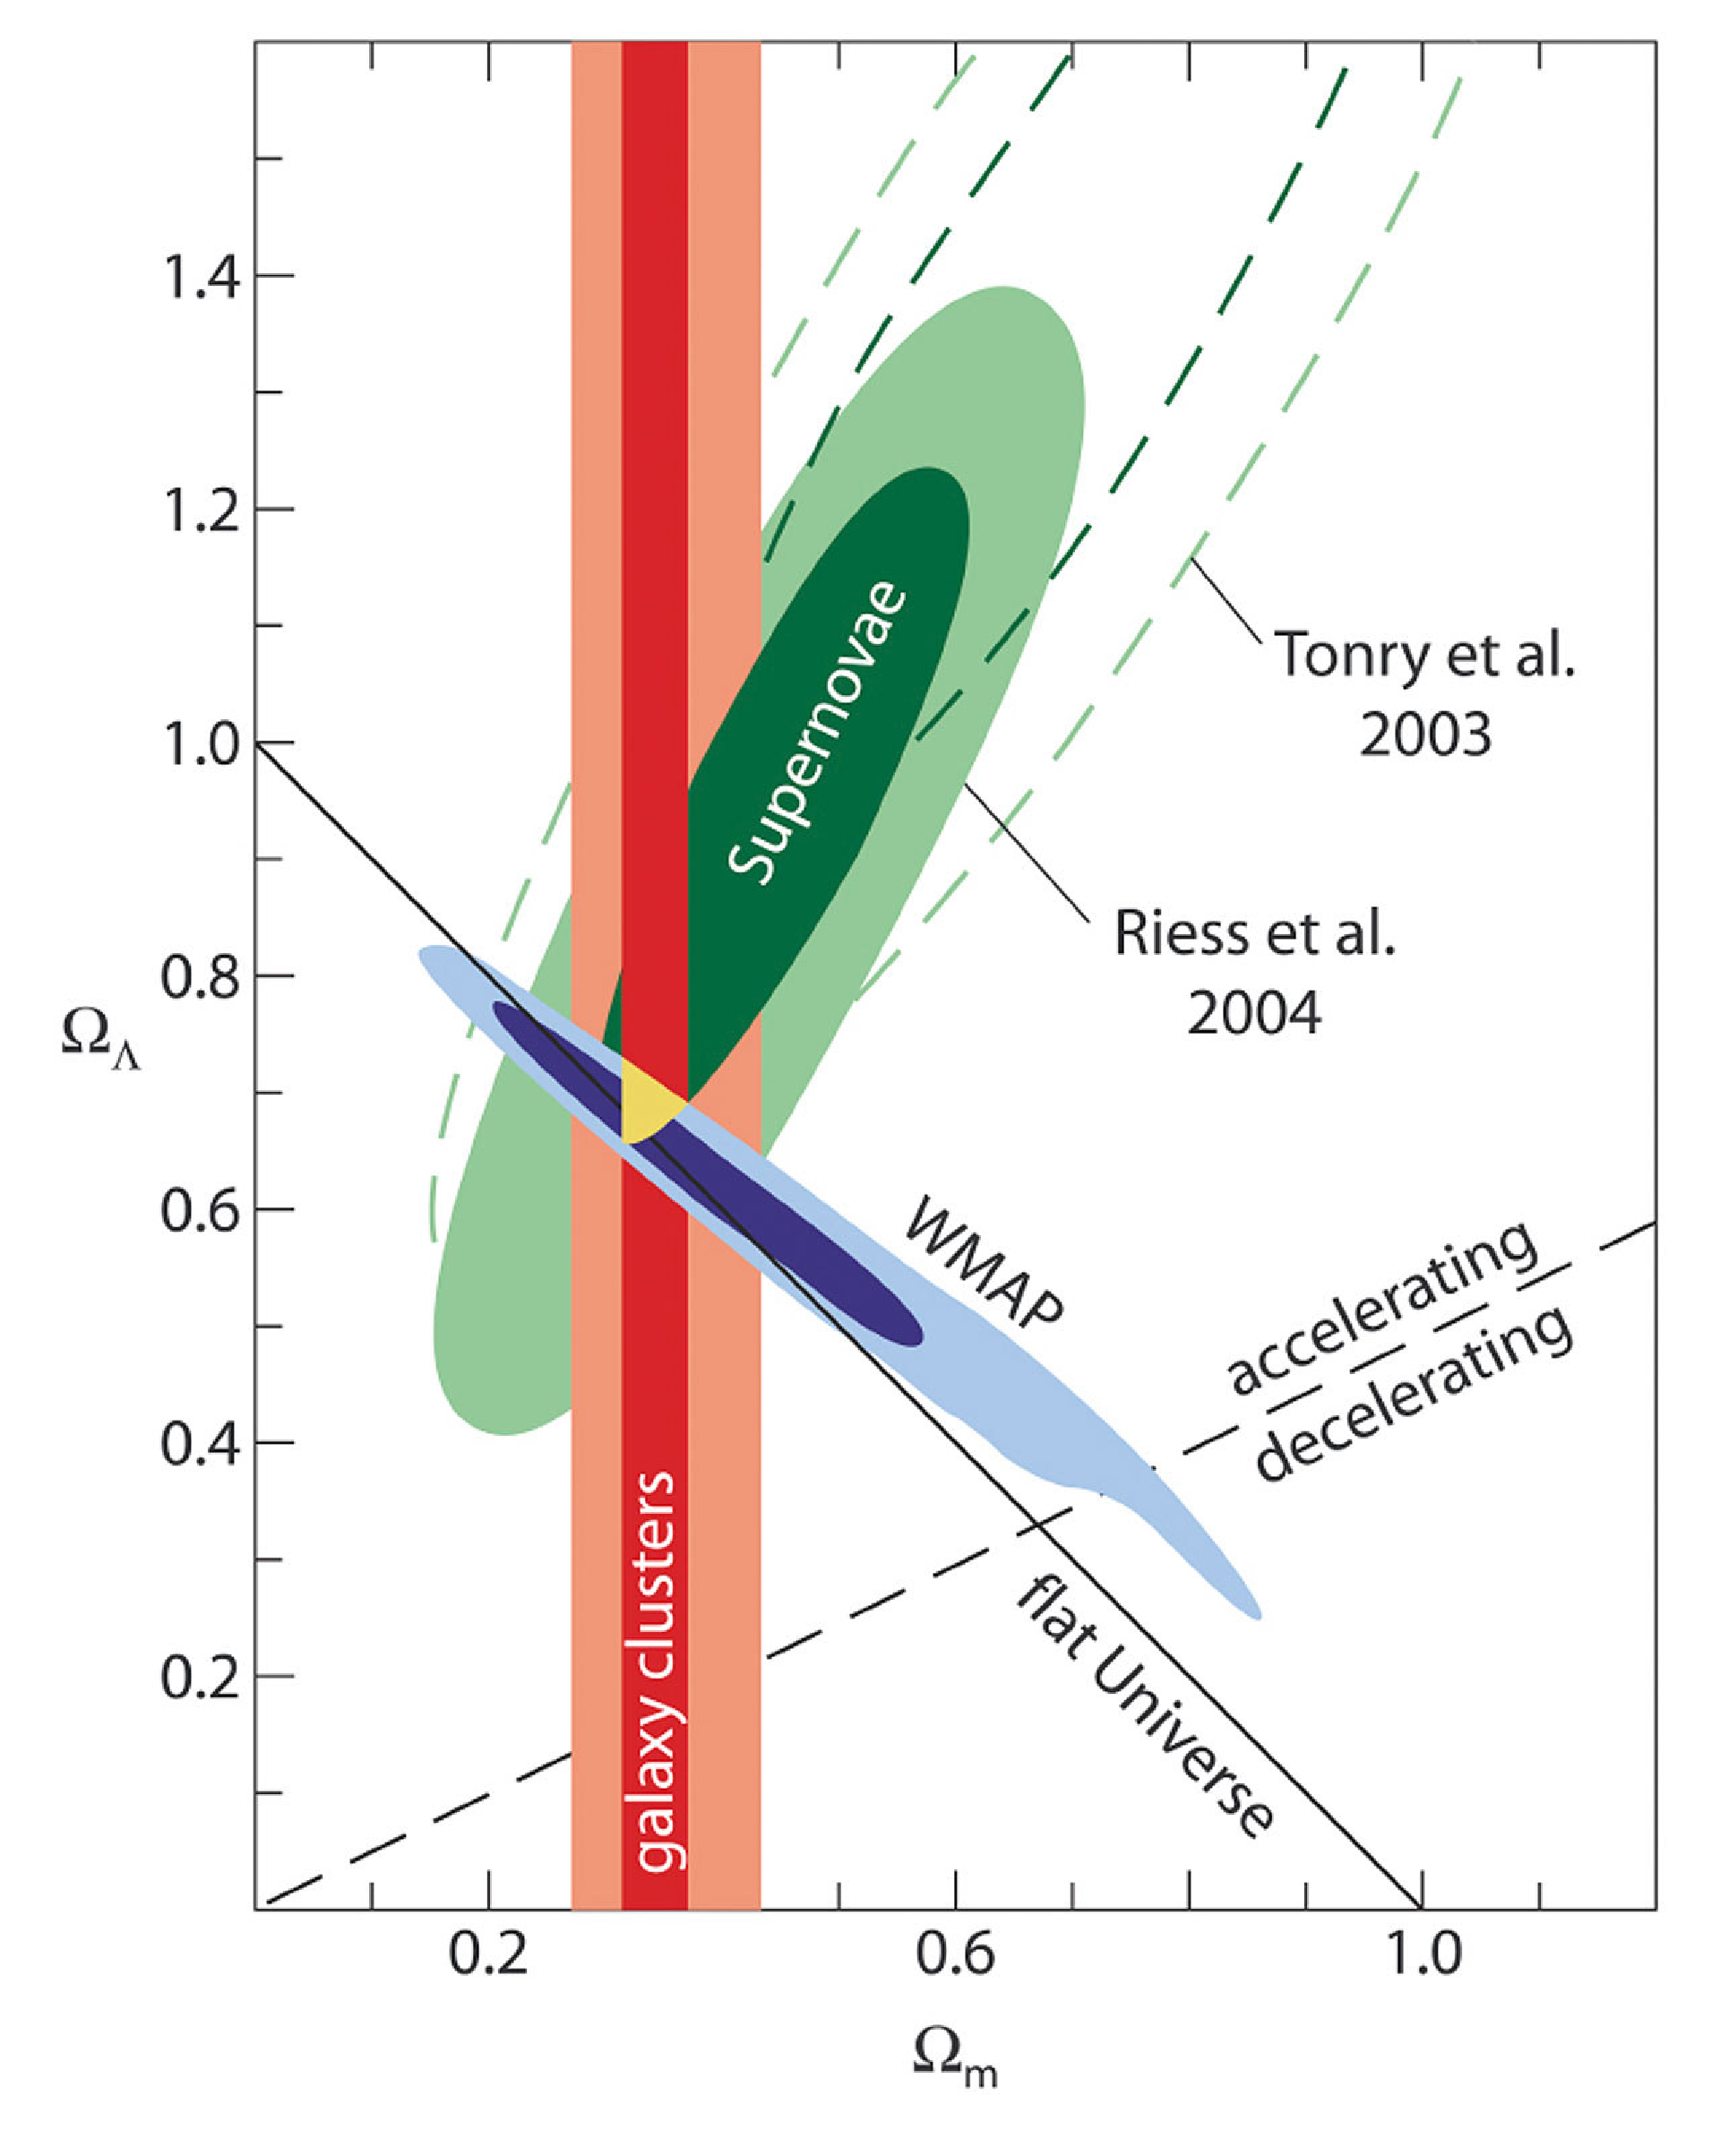
\includegraphics[width=0.6\textwidth]{figure/Cosmological_parameters.pdf}
  \caption{Spazio dei parametri $\Omega_{m}$, $\Omega_{\Lambda}$, $\Omega_k$}
  \label{fig:Par_Cosm}
\end{figure}

\subsubsection{Dark Energy}

Dal punto di vista fenomenologico, invece di introdurre nelle eq. di Einstein (a
sinistra) il termine $g_{\mu \nu}\Lambda$, possiamo introdurre (a destra) un
termine di sorgente con densità $\rho_{DE}$, che attribuiamo ad una nuova
componente dell'Universo nota come Dark Energy.  In generale si assume che la
Dark Energy abbia eq. di stato $p_{DE}=w\rho_{DE}$ con $w<0$.  Il caso $w=-1$
corrispondente alla costante cosmologica.  Ora, se assumiamo che la componente
DE sia disaccoppiata dalla radiazione
\begin{equation}
  \toder{(\rho_{DE} R^3)}{R} = -3 p_{DE} R^2
\end{equation}
si ha
\begin{equation}
  \rho_{DE} \propto \frac {1}{R^{3(1+w)}}
\end{equation}
Pertanto $\rho_{DE}=\text{cost}$ implica $w=-1$ come per il caso
$\rho_{\Lambda}=\text{cost}$, $p_{\Lambda}=-\rho_{\Lambda}$.

Notiamo che il rapporto $\rho_{DE}/\rho_m \propto R^{-3w} \propto (1+z)^{3w}$.
Quindi nel caso $w<0$, per $t < t_0 $ ($z$ crescente a partire dal valore 0), si
ha $\rho_{DE}/\rho_m \to 0$, cioè l'importanza della componente DE diminuisce
indietro nel tempo e i risultati dei modelli di Friedmann non sono modificati
per $z\gg 1$ dalla presenza della componente DE.

L'eq. \eqref{hzcc} risulterà così modificata:
\begin{equation}
  H(z)=H_0 \left[ \Omega_{DE} (1+z)^{3(1+w)} + \Omega_{k} (1+z)^2+ \Omega_m
    (1+z)^3 \right]^{1/2}
  \label{hzccX}
\end{equation}

Anche l'eq. (\ref{ddRcc}) è modificata
\begin{equation}
  \frac {\ddot{R}} {R} = H_0^2
  \left[ - \frac{\Omega_{DE} (1+3w)}{2} (1+z)^{3(1+w)}
    -\frac {\Omega_m (1+z)^3} {2 } \right]
  \label {ddRw}
\end{equation}
da cui per il parametro di decelerazione si ha ora
\begin{equation}
  q_0= \frac{\Omega_{DE}}{2} (1+3w) +  \frac{\Omega_m}{2} + \Omega_{k}
\end{equation}
e, nel caso $k=0$ (poichè $\Omega_m = 1 - \Omega_{DE}$), si ha
\begin{equation}
  q_0= \frac {1+3w \Omega_{DM}}{2},
\end{equation}
per cui se poniamo $\Omega_{DE} \simeq 0.7$ si ha $q_0 =0.5+w$ che diventa
negativo (quindi l'Universo oggi è in una fase di espansione accelerata) se
$w<-0.5$.  In realtà lo studio dei diagramma di Hubble $m-z$ non permette una
precisa determinazione del valore di $w \simeq -0.7$ a causa delle larghe
incertezze dei dati osservativi.

%Tornando indietro alla relazione $d_L(z)$ osserviamo che nel caso $\Omega_{k}=0$
%ed $\Omega_{\Lambda}=0$
%\begin{equation}
%d_L =
%\end{equation}
%mentre se prendo $\Omega_{k}=0$ ed  $\Omega_{m}=0$
%\begin{equation}
%d_L = (1+z) \int_0^z \frac{dz}{H_0 (1+z)^{3(1+w)/2}}
%\end{equation}
%e per $w=-1$ segue $d_L=H_0^{-1} z (1+z)$. Quindi a parità di $z$ oggetti
%appaiono più o meno distanti a seconda del valore dei parametri cosmologici
%$\Omega$.  Vedi figura da cui si ottiene (assumendo $k=0$ $\Omega_{m}=0.32$ ed
%$\Omega_{\Lambda}=0.68$)

L'introduzione della costante cosmologica nelle eq. di Einstein
può essere interpretata in due modi:
\begin{itemize}
\item nel primo caso è come se la lagrangiana della materia sia modificata con
  l'aggiunta di un termine costante
  \begin{equation}
    L_{\textup{matter}} \to L'_{\textup{matter}} = L_{\textup{matter}} -
    \frac{\Lambda}{8 \pi G},
  \end{equation}
  così che l'integrale d'azione diventa
  \begin{equation}
    S_{tot}=S_{g}+S_{m}= \frac {1}{16 \pi G} \int R \sqrt{-g} \dd^4x + \int
    \left( L_{m}- \frac {\Lambda}{8 \pi G} \right) \sqrt{-g} \dd^4 x.
  \end{equation}
  L'eq. del moto per la materia (descritta dal campo $\phi$) che sono ottenute
  variando $S$ rispetto $\phi$ e ponendo $\delta S/\delta \phi=0$, rimangono
  inalterate poiché $\Lambda=\text{cost}$.  In questo caso l'introduzione del
  termine $\Lambda$ introduce solamente uno shift nel livello zero dell'energia
  della materia e non influenza la dinamica della materia, mentre la gravità che
  è accoppiata alla energia totale del sistema ne è influenzata;
\item il secondo caso corrisponde ad un integrale d'azione scritto come
  \begin{equation}
    S_{tot}= \frac {1}{16 \pi G}
    \int (R-2\Lambda)  \sqrt{-g} \dd^4x + \int  L_{m} \sqrt{-g} \dd^4 x,
  \end{equation}
  e la gravità risulta descritta dalle due costanti $G$ e $\Lambda$.  In questo
  secondo caso lo spazio-tempo è curvo anche in assenza di materia.
\end{itemize}

L'eq. di stato $\rho=-p$ ha un'altra importante implicazione in relatività
generale.  La parte spaziale $\bm{g}$ dell'accelerazione geodetica (che misura
l'accelerazione di due particelle di prova molto vicine) soddisfa l'eq.
\begin{equation}
  \nabla \cdot \bm{g} = - 4 \pi G (\rho+3p)~,
\end{equation}
per cui la causa dell'accelerazione geodetica è $\rho+3p$.  Quindi se
$\rho+3p<0$, la gravità diventa repulsiva.

Questo starebbe accadendo oggi nell'Universo poichè all'istante attuale la DE
domina ($\rho_{\Lambda}+3 p_{\Lambda} <0$).  La transizione dalla gravità
attrattiva (dovuta alla materia ordinaria) a quella repulsiva avverrebbe a un
red-shift $\simeq 0.5$.

Quanto vale $\Lambda$?  Preliminarmente osserviamo che $\Lambda$ ha dimensioni
cm$^{-2}$.  La velocità della luce e l'istante attuale $t_0$ definiscono una
lunghezza caratteristica (raggio visibile dell'Universo nel caso $k=1$) $l_0 = c
t_0 \simeq c/H_0 \simeq 10^{28}$ cm $\simeq$3 Gpc.  Poiché l'Universo appare
omogeneo ed isotropo su questa scala (non vi sono effetti indotti da $\Lambda$
nella distribuzione di sorgenti) $\Lambda < 10^{-56}$ cm$^{-2}$.

\section{Radiazione di fondo cosmico}

La radiazione di fondo cosmico nella banda delle microonde (CMB) ha uno spettro
di corpo nero a $T_{CMB}(0) \simeq 2.725$K.  Nella Figura~\ref{fig:radio-gamma}
lo spettro della radiazione extragalactica è mostrato in funzione dell'energia
dei fotoni.  La CMB contribuisce con il 93\% dell'emissione totale.  Definita la
grandezza $f_{\lambda}= \rho_{\lambda}/\rho_{tot}$, si ha:
$f_{CMB}=0.93,$ $f_{IR}= 0.05$, $f_{VIS}=0.02$, $f_{X}=2.5
\times 10^{-4},$ $f_{\gamma}= 2.5 \times 10^{-5}$, $f_{CR} \simeq
\Omega_{CMB}$.
\begin{figure}
  \centering{}
  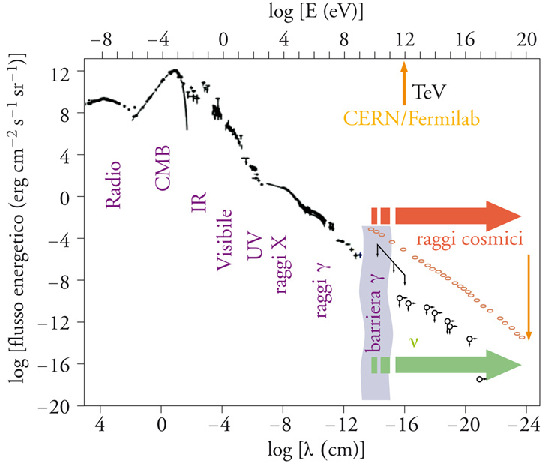
\includegraphics[width=0.8\textwidth]{figure/Radiazione_radio_gamma.pdf}
  \caption{Radiazione dal radio al gamma}
  \label{fig:radio-gamma}
\end{figure}
\begin{figure}
  \centering{}
  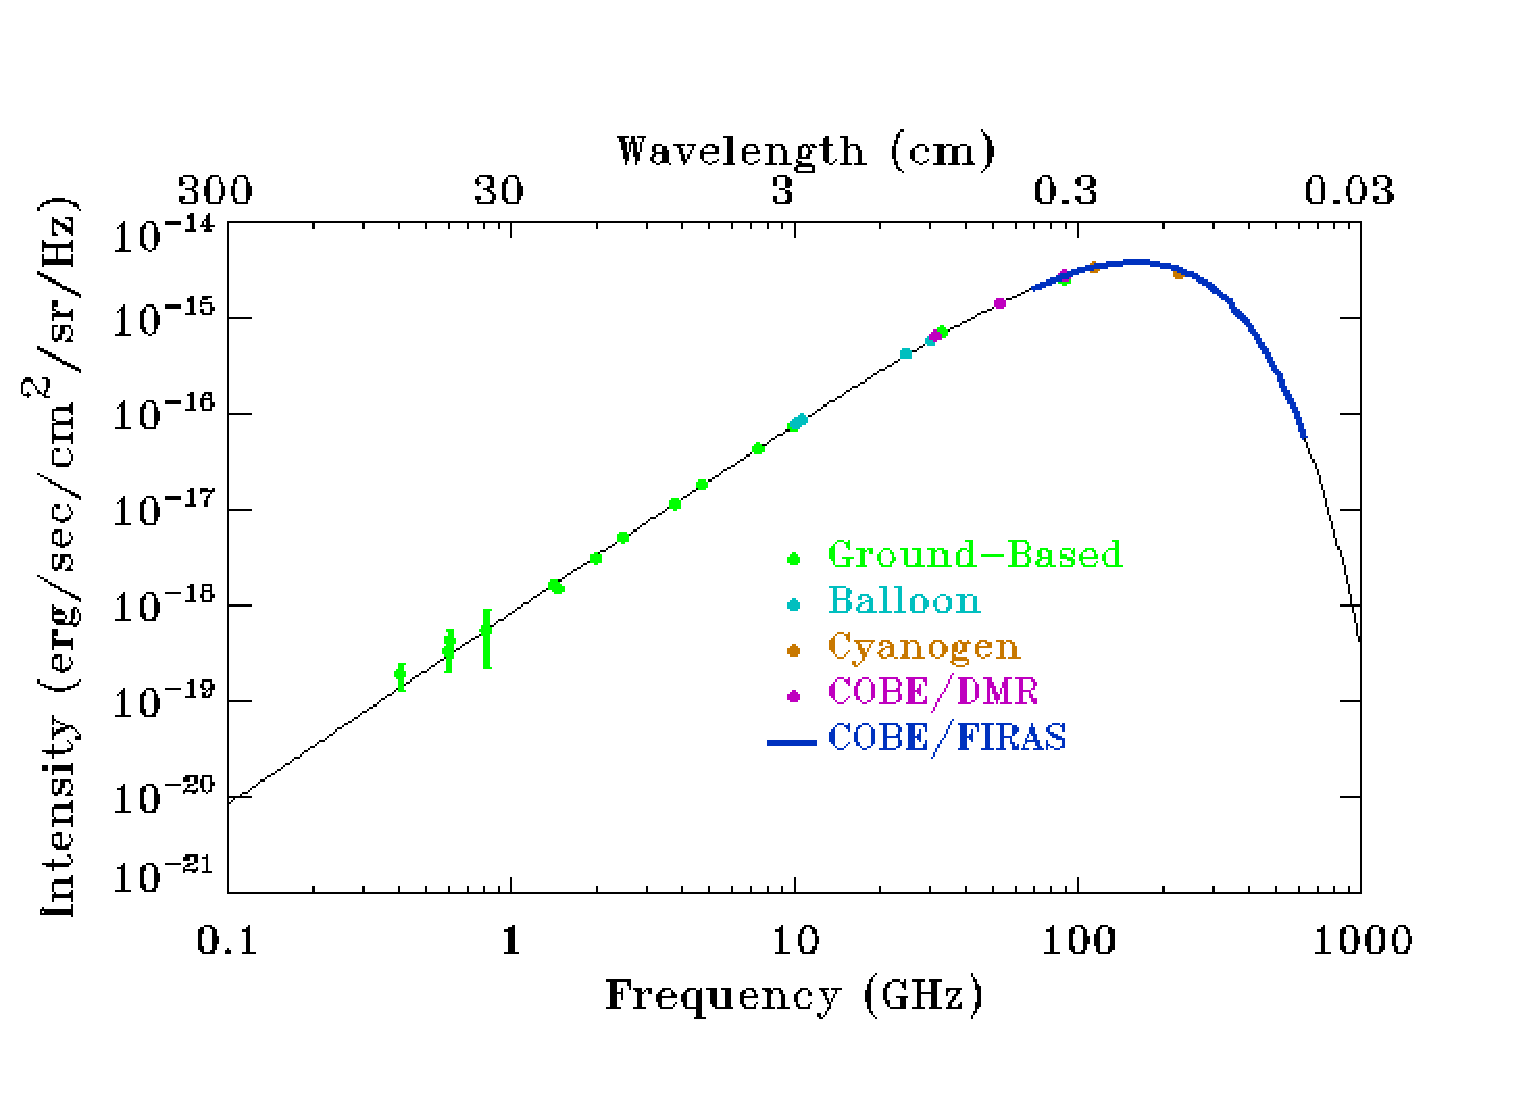
\includegraphics[width=\textwidth]{figure/CMB_intensity.pdf}
  \caption{CMB e distribuzione di Planck a $T_{CMB} = 2.75$K}
  \label{fig:spettro_CMB}
\end{figure}
La densità di energia di un gas di bosoni è
\begin{equation}
  d \rho (p)  = g \frac{4 \pi p^2 dp} {h^3} \frac{1} {\exp[ E(p) / kT ]-1} E(p)
\end{equation}
e poichè (i fotoni sono bosoni di massa nulla) $E(p)=pc=h\nu$ e $g=2$, si ha
\begin{equation}
  d \rho_{\gamma}(\nu) =   \frac{8 \pi h \nu^3 } {c^3} \frac{1} {\exp(h \nu/ kT)
    -1} d\nu
  \label{spettro_BB}
\end{equation}

Posto $x=(h \nu/kT)$, nello spettro di corpo nero si distingue la regione di
Rayleigh-Jeans (con $x\ll 1$) in cui lo spettro cresce come $x^2$ e la regione
di Wien con spettro decrescente come $x^3 \exp(-x)$.  Il massimo dello spettro
si trova derivando l'eq.  \eqref{spettro_BB} rispetto ad $x$ e uguagliando a
zero.  Si ottiene $3(\exp x_{max} -1) = x_{max} \exp(x_{max})$, che ha soluzione
numerica $x_{max} \simeq 2.8$. Quindi $(h \nu_{max}) \simeq 2.8 kT_{max}$, da
cui $(h \nu_{max}) \simeq 2.4 \times 10^{-4}$ eV o, equivalentemente,
$\lambda_{max} \simeq 1.7$ mm, $\nu_{max} \simeq 1.8 \times 10^{11}$ Hz.

La densità totale di energia si calcola integrando lo spettro su tutte le
frequenze
\begin{equation}
  \begin{split}
    \rho_{\gamma}(t_0) &= \int_0^{\infty} \frac{8 \pi h \nu^3 } {c^3}
    \frac{\dd\nu} {\exp (h \nu/
      kT_0) -1} \\
    &= \frac{8 \pi k^4 T^4_0}{c^3 h^3} \int_0^{\infty} \frac{x^3}{e^{x} -1} \dd
    x \\
    & = a T^4_0 \\
    & = 4.64 \times 10^{-34}~~{\rm gr~cm^{-3}} \implies \Omega_{\gamma} =2.47
    \times 10^{-5} h^{-2}
\end{split}
\end{equation}
dove $a=(8 \pi k^4)/(15 h^3 c^3) = 7.56 \times 10^{-15}$ erg cm$^{-3}$
deg$^{-4}$ è la costante di Stefan-Boltzmann, e $h$ è la costante di Hubble in
unità di $100$ km/sec/Mpc, cioè $h=H_0/100$ km/sec/Mpc.

La densità spaziale di fotoni della CMB all'istante attuale è
\begin{equation}
  \begin{split}
    n_{\gamma}(t_0) & = \int_0^{\infty} \frac{\rho_{\gamma}(t_0) } {h \nu }
    \dd\nu
    = \frac{8 \pi k^3 T^3_0 }{c^3 h^3} \int_0^{\infty} \frac{x^2}{e^x -1} \dd x
    \\
    & = \frac{30 a \zeta(3) T^3_0} {\pi^4 k} = 0.3702 \frac{a T^3_0}{k} = 410
    ~{\rm fotoni/cm^3}
  \end{split}
\end{equation}
L'attuale  densità di nucleoni  è invece
\begin{equation}
  n_N (t_0) = \frac{3 \Omega_B H_0^2}{8 \pi G m_N c^2} =
  1.123 \times 10^{-5} \Omega_B h^2 ~{\rm nucleoni/cm^3}
\end{equation}
e il rapporto tra le due densità rimane costante nel tempo (perché entrambe
variano come $\propto R^{-3}$)
\begin{equation}
  \frac{n_{\gamma}(t_0)}{n_N(t_0)} = 3.65 \times 10^{7}.
\end{equation}

A temperature $T>4000~$K l'Universo è opaco alla radiazione con $\gamma$, H$^+$,
e$^-$ in contatto termico alla stessa temperatura e $\gamma$ con spettro di
corpo nero; a $T \simeq 4000$K si forma l'idrogeno neutro e l'Universo diventa
trasparente alla radiazione, nel senso che l'assorbimento di un fotone alla
frequenza $\nu= \Delta E/h$ è seguito da emissione isotropa di un fotone alla
stessa frequenza.

Ma lo spettro continua ad essere di corpo nero. Per dimostrarlo, supponiamo che
la transizione tra Universo opaco e Universo trasparente avvenga istantaneamente
al tempo di ultimo scattering $t_{LS}$ a cui la temperatura ha il valore
$T_{LS}$.

Se consideriamo tempi successivi $t>t_{LS}$ abbiamo le seguenti proprietà
\begin{itemize}
\item fotoni che al tempo $t$ hanno frequenza $\nu$, a $t_{LS}$ avevano
  frequenza (maggiore) $\nu R(t)/R(t_{LS})$
\item a causa dell'espansione la densità propria di fotoni diminuisce come
  $[R(t_{LS})/R(t)]^3$.
\end{itemize}
Quindi, al tempo $t$ la densità di fotoni con frequenza tra $\nu$ e $\nu+d\nu$ è
determinata a partire dalla densità al tempo $t_{LS}$ modificata dalle proprietà
precedenti:
\begin{equation}
  n_{\gamma}(\nu, t) d\nu = \left( \frac {R(t_{LS})} {R(t)} \right)^3
  8 \pi \nu^2 d \nu
  \left( \exp \left[ \frac {h} {k T_{LS}} \frac{\nu R(t)}{R(t_{LS})} \right] -1
  \right)^{-1} \left( \frac {R(t)} {R(t_{LS})} \right)^3
\end{equation}
da ciò si vede che $n_{\gamma}(\nu,t)$ è una distribuzione di corpo nero a ogni
$t$ se
\begin{equation}
  T(t) = T_{LS} \frac {R(t_{LS})} {R(t)}
\end{equation}

Questa conclusione è inalterata se la transizione dall'opacità alla trasparenza
avviene in un tempo finito poichè l'interazione $\gamma H$ è limitata allo
scattering elastico per il quale le frequenze dei $\gamma$ non cambiano.

Dopo il disaccoppiamento tra materia e radiazione si ha $\rho_{\gamma} \propto
R^{-4}$ e poiché $\rho_{\gamma} \propto T^4$, si ha $T_{\gamma} \propto
R(t)^{-1}$.  Ma prima del disaccoppiamento come varia la temperatura dei fotoni
in contatto termico con la materia?  A questo scopo consideriamo un semplice
modello per l'Universo che supponiamo costituito da un gas ideale e radiazione
alla stessa temperatura $T_{\gamma}=T_{m}=T$. Densità e pressione delle due
componenti sono
\begin{subequations}
  \begin{align}
    \rho_{\gamma} & = a T^4 \\
    p_{\gamma} &=\rho/3  \\
    \rho_{m}    & = n_N m c^2 + \frac{p_{m}}{\gamma-1} \\
    p_m &=n_N kT
  \end{align}
\end{subequations}
dove l'indice politropico $\gamma=5/3$ $(4/3)$ per il regime non relativistico
(relativistico).  Per la densità e pressione totali avremo $\rho =
\rho_{m}+\rho_{\gamma}$ e $p=p_{m}+p_{\gamma}$ e sostituendo
nell'eq. \eqref{moto} si trova l'eq. differenziale
\begin{equation}
  \label{TvsR}
  \frac{R}{T} \toder{T}{R} = -
  \left(\frac{\sigma+1}{\sigma+[3(\gamma-1)]^{-1}}\right)
\end{equation}
dove la costante $\sigma = 4 a T^3_{\gamma}/(3 n_N k)$ è l'entropia specifica.  Ora:
\begin{itemize}
\item se $\sigma \ll 1$, dall'eq. \eqref{TvsR} segue $T \propto
  R^{-3(\gamma-1)}$ che è l'usuale relazione temperatura-volume per
  un'espansione adiabatica di un gas ideale, e infine
  $T \propto R^{-1}$ nel caso relativistico (per cui $\gamma=4/3$)
e $ T \propto R^{-2}$ nel caso non-relativistico (per cui $\gamma=5/3$);
\item se $\sigma \gg 1$ si ha sempre $T \propto R^{-1}$.
\end{itemize}

Nel nostro caso $\sigma = 4 a T^3_{\gamma}(0)/(4 n_N(0) k) \simeq 10^8$ e quindi
prima del disaccoppiamento la materia (nonostante sia in un regime
non-relativistico) segue la radiazione con $T_m=T_{CMB} \propto R^{-1}$.  Dopo
il disaccoppiamento la temperatura della materia $T_{m}\propto R^{-2}$.

\subsection{Anisotropia di dipolo}

Supponiamo che vi sia un sistema di riferimento fondamentale in cui la
radiazione di fondo cosmico sia isotropa (e con spettro di Planck) e che la
Terra si muova con velocità $v_{\oplus}$ rispetto a questo sistema.  Nel sistema
fondamentale, i fotoni nell'angolo solido $\sin \theta \dd \theta \dd \phi$ e
con frequenza tra $\nu$ e $\nu + \dd\nu$ contribuiscono al tensore energia
impulso della radiazione di fondo cosmico con
\begin{equation}
  \dd T^{\mu \nu}=  \left( \frac{p^{\mu} p^{\nu}}{h^2 \nu^2} \right)
                  \left( \frac{\sin\theta \dd\theta \dd\phi}{4\pi} \right)
  \rho_{\gamma 0}(\nu) \dd\nu
\label{521}
\end{equation}
Nella relazione precedente si è tenuto conto che il tensore energia impulso è
proporzionale a $p^{\mu} p^{\nu}$ (vedi~\cite[44]{weinberg:gravitation}); gli
altri termini sono introdotti in modo che integrando sull'intero angolo solido
$\dd T^{00} = \rho_{\gamma 0} \dd \nu$.  Si ha quindi
\begin{equation}
  \dd T^{\mu \nu}= \left( 2 \frac{ p^{\mu} p^{\nu} }{h} \right)
                   \left( \frac{1} { \exp (h \nu/ kT_{\gamma 0 }) } \right)
  \sin \theta \dd\theta \dd\phi \nu \dd\nu
\label{522}
\end{equation}
con
\begin{equation}
  p^{\mu} \equiv (E, p_x, p_y, p_z) =
  h \nu ( 1, \sin \theta \cos \phi , \sin \theta \sin \phi, \cos \theta)
\end{equation}

Nel sistema della Terra il tensore energia impulso della radiazione di fondo è
\begin{equation}
  \dd T'^{\mu \nu} = \tensor{\Lambda}{^{\mu}_{\rho}} \tensor{\Lambda}{^{\nu}_{\sigma}}
  \dd T^{\rho\sigma}
\end{equation}
dove $\Lambda$ è la matrice di Lorentz con $\vec{v} = - \vec{v}_{\oplus}$.
Allora possiamo esprimere $\dd T'^{\mu \nu}$ in termini di quantità nel sistema
della Terra.  Osserviamo preliminarmente
\begin{equation}
  p'^{\mu } = \tensor{\Lambda}{^{\mu}_{\nu}} p^{\nu}
\end{equation}
e che orientando gli assi in modo ($\phi=0$) che l'asse z sia nella direzione della
velocità della Terra,  si ha
\begin{subequations}
  \begin{gather}
    \nu' = \nu \frac{[1-v_{\oplus}\cos\theta]}{[ 1 - v_{\oplus}^2]^{1/2}}, \\
    \cos\theta' = \frac{[- v_{\oplus} + \cos\theta]}{[1 - v_{\oplus}
      \cos\theta]}, \\
    \phi' = \phi
  \end{gather}
\end{subequations}
dove ora $\theta$ è l'angolo tra la velocità della Terra e il fotone.
Il tensore energia impulso differenziale nel sistema terra ha necessariamente la forma
\begin{equation}
  \dd T^{\prime \mu \nu}= \left( 2 \frac{ p^{\prime \mu} p^{\prime \nu} }{h} \right)
                   \left( \frac{1} { \exp (h \nu/ kT_{\gamma 0 }) } \right)
  \sin \theta \dd\theta \dd\phi \nu \dd\nu
\end{equation}
poiché in eq.~\eqref{522} il termine a sinistra è un tensore di rango 2
controvariante, il prodotto $p^{\mu} p^{\nu}$ è un tensore dello stesso tipo e
rango e quindi la parte restante a destra è un invariante.  Ora, l'angolo solido
ha la regola di trasformazione (?)
\begin{equation}
 \sin \theta^{\prime} \dd\theta^{\prime} \dd\phi^{\prime}
= \left( \frac {\nu}{\nu^{\prime}} \right)^2 \sin \theta \dd\theta \dd\phi
\end{equation}
da cui segue
\begin{equation}
  \dd T^{\prime \mu \nu}= \left( 2 \frac{ p^{\prime \mu} p^{\prime \nu} }{h} \right)
                   \left( \frac{1} { \exp (h \nu^{\prime}/ kT^{\prime}_{\gamma 0 }) } \right)
  \sin \theta^{\prime} \dd\theta^{\prime} \dd\phi^{\prime} \nu^{\prime} \dd\nu^{\prime}
\end{equation}
dove si \'e posto
\begin{equation}
T^{\prime}_{\gamma 0} \equiv \left( \frac{\nu ^{\prime}}{\nu} \right) T_{\gamma 0} =
\left[ \frac{(1- v_{\oplus} \cos \theta)}{(1-v_{\oplus}^2)^{1/2} } \right] T_{\gamma 0}
\end{equation}
Quindi, rispetto alla Terra la radiazione di fondo cosmico ha ancora una distribuzione di Planck
ma con una temperatura differente.
Per velocit\'a piccole, cio\'e per $v_{\oplus}/c << 1$, segue che
\begin{equation}
\Delta T_{\gamma 0} = T^{\prime}_{\gamma 0} - T_{\gamma 0} = - \frac{ v_{\oplus}} {c} T_{\gamma 0}
\end{equation}
Questa relazione determina un'anisopropia di dipolo in due direzioni opposte.
Da misure recenti si trova $v_{\oplus} \simeq 300$ km/s (nel direzione ....) e quindi
$  \Delta T_{\gamma 0} / T_{\gamma 0} \simeq 10^{-3}$.

\subsection{Effetto GZK}

I raggi cosmici, prevalentemente protoni, sono prodotti da acceleratori cosmici
(SN galattiche fino ad energia $E_{CR} \simeq 10^{15}$ eV, AGN extragalattici
per energie maggiori) ed hanno uno spettro che si estende da circa $10^9$ ev fino a $10^{21}$ ev
seguendo semplici leggi di potenza. (Vedi Fig. \ref{fig:CR1})
 \begin{figure}
   \centering{}
   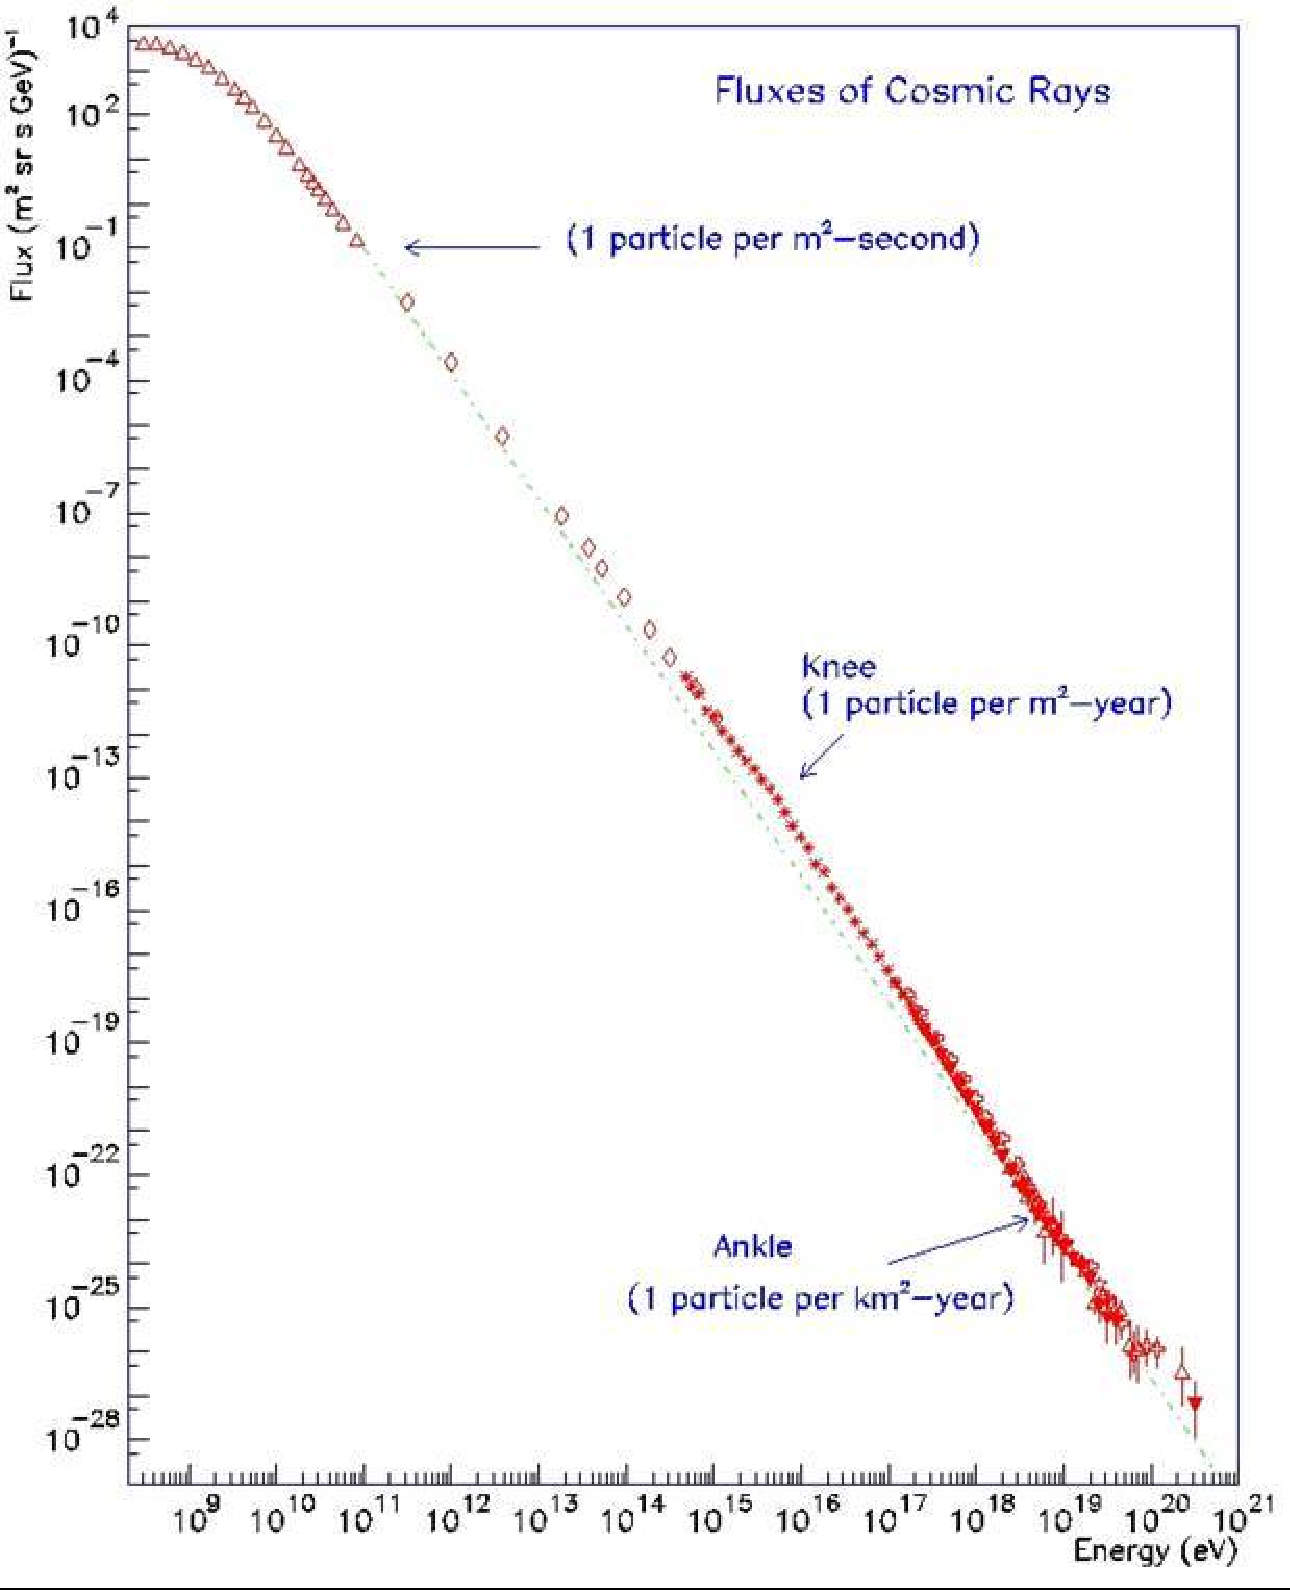
\includegraphics[width=0.8\textwidth]{figure/CR_spectrum_1.pdf}
  \caption{Spettro dei Raggi Cosmici}
  \label{fig:CR1}
\end{figure}
Comunque ad energie $E_{CR} \simeq 10^{20}$ eV si osserva nello spettro dei CR
una perdita di flusso che è una dimostrazione indiretta dell'esistenza della
CMB: protoni di alta energia interagiscono con i fotoni del fondo cosmico dando
luogo ad interazioni forti del tipo $p \gamma_{CMB} \to p \pi^0$ e $\gamma_{CMB}
p \to n \pi^+$, e quindi non ci raggiungono.  Tali processi, comunque, avvengono
attraverso la creazione di risonanze (stati metastabili intermedi)
$\Delta^{++}$, $\Delta^{+}$, $\Delta^{0}$ e il loro successivo decadimento.
L'effetto è stato predetto
da~\textcites{1966PhRvL..16..748G}{1966JETPL...4...78Z}.

La massa della risonanza $m_{\Delta} \simeq 1236$ MeV pone un limite inferiore
all'energia dei protoni dei CR capaci di attivare il processo di annichilazione.
Consideriamo la cinematica del processo.  Nel sistema del laboratorio sia
\begin{subequations}
  \begin{align}
    P^{\mu}_{\gamma}       &= (q, \bm{q}), \\
    P^{\mu}_{\ \textup{p}}   &= (\sqrt{p^2+m^2_\textup{p}}, \bm{p}), \\
    P^{\mu}_{\ \textup{tot}} &= ( q+\sqrt{p^2+m^2_\textup{p}}  ,  \bm{q} + \bm{p}) \\
    \sqrt{s} &= \sqrt{ P^{\mu}_{\ \textup{tot}} P_{\mu \ \textup{tot}} } =
                        \left[ \left( q+\sqrt{p^2+m^2_\textup{p}} \right)^2 -
                        \left(\bm{q}+ \bm{p} \right)^2 \right]^{1/2} \\
                      & \simeq \left[ 2qp \left(1-\cos \theta \right) +
                        m_\textup{p}^2 \right]^{1/2}.
  \end{align}
\end{subequations}
La reazione può avvenire se $\sqrt{s} > m_{\Delta} c^2$.  La tipica energia
$\langle E_{\gamma}\rangle$ dei fotoni della CMB è $6 \times 10^{-4}$ eV e il
massimo di $(1-\cos \theta)=2$.  Si ha quindi
\begin{equation}
  p_{\textup{th}} \simeq \frac{m^2_{\ \Delta} c^4 - m^2_{\ p} c^4} {4 \langle
    \ E_{\gamma}\rangle} \simeq 10^{20}~~~{\rm eV}
\end{equation}
Nella figura~\ref{fig:CR2} è riportato lo spettro dei raggi cosmici attorno al
taglio GZK.
\begin{figure}
  \centering{}
  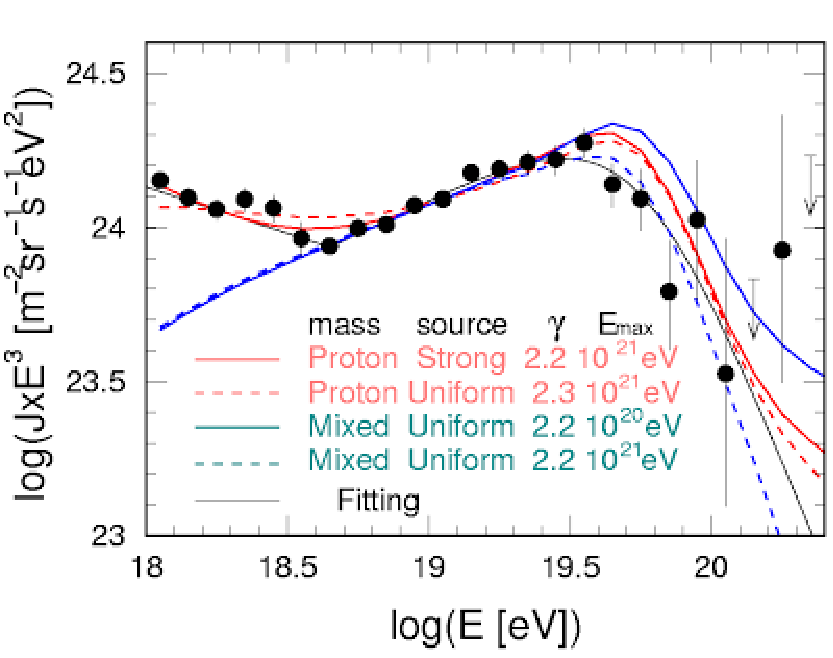
\includegraphics[width=\textwidth]{figure/CR_spectrum_2.pdf}
  \caption{Spettro dei Raggi Cosmici a $E \simeq 10^{20}$ eV}
  \label{fig:CR2}
\end{figure}

\section{Conservazione dell'entropia}

Si consideri un gas perfetto con densità e pressione $\rho= \rho(T)$ e $p=p(T)$.
Le leggi della termodinamica sono
\begin{subequations}
  \label{leggi_termo}
  \begin{align}
    \dd Q &= \dd U+p\dd V \\
    \dd S &= \frac{\dd Q}{T}
  \end{align}
\end{subequations}
in cui $dQ$ è il calore assorbito, $dU=d(\rho c^2 V)$ la variazione di energia
interna, $pdV$ il lavoro eseguito, $dS$ la variazione di entropia, $V$ infine è
il volume occupato dal gas.

Dalle leggi della termodinamica si ha
\begin{equation}
  \begin{split}
    \dd S &=  \frac{1}{T} \left( \dd( \rho c^2 V) + p \dd V \right) \\
    &= \frac{1}{T} \left( V \dd(\rho c^2) + (\rho c^2+p) \dd V \right) \\
    &= \frac{1}{T} \left( V \toder{(\rho c^2)}{T} \dd T + (\rho c^2+p) \dd V
    \right).
  \end{split}
\end{equation}
Poichè $S=S(V,T)$ segue
\begin{equation}
  \dd S = \left( \frac{\partial S}{\partial T} \right)_V \dd T +
  \left( \parder{S}{V} \right)_T \dd V
\end{equation}
dal confronto tra le precedenti eq. si ha
\begin{subequations}
  \begin{align}
    \left(\parder{S}{V}\right)_T &= \frac{1}{T} (\rho c^2+p) \\
    \left(\parder{S}{T}\right)_V &= \frac{V}{T} \toder{(\rho c^2)}{T}.
  \end{align}
\end{subequations}
La condizione di integrabilità
\begin{equation}
  \frac{\partial}{\partial T} \left( \frac{\partial S}{\partial V} \right) =
  \frac{\partial}{\partial V} \left( \frac{\partial S}{\partial T} \right)
\end{equation}
conduce alla relazione
\begin{equation}
  \toder{p}{T} = \frac{1}{T} (\rho c^2 +p).
  \label{integrab}
\end{equation}
Usando questa relazione nella legge di conservazione dell'energia \eqref{moto}
si ha
\begin{equation}
  \begin{split}
    \toder{}{t} [R^3(\rho c^2 +p)] & = R^3 \toder{p}{t} \\
    & = R^3 \toder{p}{T} \toder{T}{t} \\
    & = R^3 (\rho c^2 +p) \frac{1}{T} \toder{T}{t}
  \end{split}
\end{equation}
da cui segue
\begin{equation}
  \toder{}{t} \left( \frac{R^3}{T} (\rho c^2 + p) \right) = 0.
\end{equation}
Se indichiamo con $S(t)$ l'entropia contenuta nel volume comoving, abbiamo
\begin{subequations}
  \begin{align}
    S(t) & =  \left( \frac{R^3}{T} (\rho c^2 + p) \right) \\
    \toder{S(t)}{t} & = 0 \iff S(t)= \text{cost}
  \end{align}
  \label{cons_entropia}
\end{subequations}
che esprime la conservazione dell'entropia contenuta in un volume comoving (che
scala come $R^3$).

Verifichiamo che la definizione di $S$ è consistente con la $2^a$ legge della
termodinamica in eq. \eqref{leggi_termo}, che riscriviamo nella forma
\begin{equation}
  \dd S  = \frac{1}{T} \left( \dd(\rho c^2 V) + \dd(pV) - V \toder{p}{T} dT
  \right)
\end{equation}
e usando l'eq. \eqref{integrab}
\begin{equation}
  \begin{split}
    \dd S &= \frac{1}{T} \left( \dd(\rho c^2 V + pV) -  \frac{V}{T}   (\rho c^2
      +p) \dd T \right) \\
    &= \dd\left( \frac{V (\rho c^2 + p)} {T}  \right)
  \end{split}
\end{equation}
che è la relazione in eq. \eqref{cons_entropia} poiché $V \propto R^3$.

\section{Universo primordiale}

Si prende ora in esame l'era dell'Universo dominata dalla radiazione, per cui
\begin{equation}
  \rho(t)=\rho_0 \left(\frac{R_0}{R(t)} \right)^4
  \label{293}
\end{equation}
La dinamica dell'Universo è descritta dall'eq. \eqref{eq:friedmann}, in cui ora
però si può trascurare il termine $k$
\begin{equation}
  \dot{R}^2 = \frac{8 \pi G}{3} \rho R^2,
  \label{fri_pri}
\end{equation}
in quanto il termine $(8 \pi G /3) \rho R^2$ risulta essere $\gg 1$ nell'era
della radiazione.  Infatti, all'istante attuale $t_0$ si ha
\begin{equation}
  \frac{8 \pi G}{3} \rho_0 R^2_0 = \frac{2q_0}{|2q_0-1|} > 0.03
\end{equation}
poichè $q_0>0.014$.  D'altra parte indietro nel tempo, tale termine cresce
almeno come $z$ e quando $z\simeq 1000$ (inizio era radiazione) risulta $>30$.

Da eq. \eqref{293} e \eqref{fri_pri} si ha
\begin{equation}
  \frac{\dot \rho}{\rho} = -4 \frac{\dot R}{R} = - 4 \left( \frac{8 \pi G
      \rho}{3} \right)^{1/2}
\end{equation}
da cui segue la relazione tra $t$ e $\rho$
\begin{equation}
  t = \left( \frac{3}{32 \pi G \rho} \right)^{1/2} + \text{cost}\ .
  \label{tvsrho}
\end{equation}

L'obiettivo ora è quello di ricavare $\rho= \rho(T)$.  Ovviamente ci riferiamo
ad un era in cui le galassie non si erano ancora formate ed il fluido
cosmologico è diffuso con densità (quasi) uniforme.  In realtà all'interno della
materia (prevalentemente dark) e della radiazione sono presenti (i semi delle
galassie) le fluttuazioni di densità (prodotte da transizioni di fase tra
$10^{-43} - 10^{30} sec$, durante l'epoca inflazionaria) che si accrescono a
causa del meccanismo di Jeans (instabilità gravitazionali di sistemi di
dimensioni maggiori della lunghezza d'onda di Jeans).  Al disaccoppiamento,
comunque, i contrasti di densità sono ancora molto piccoli, poiché $\Delta \rho
/ \rho \simeq \Delta T / T \simeq 10^{-5}$ durante l'era in cui ci è contatto
termico tra materia e radiazione. I picchi di densità successivamente si
accrescono fino alla creazione di strutture autogravitanti di materia oscura. Si
formano quindi prima sistemi autogravitanti di materia oscura e poi su queste
buche di potenziale gravitazionale cadono i barioni, che attraverso processi
dissipativi, alla fine danno luogo alle strutture visibili ammassi, galassie,
stelle.

A partire dal tempo a cui le interazioni deboli ed elettromagnetiche si sono separate,
$t > 10^{-30}$ secondi, $T < 100 $ Gev, i costituenti dell'Universo vanno ricercati
tra le seguenti particelle:
\begin{itemize}
\item gli adroni = barioni (n,p,..) \& mesoni ($\pi$, k, ...) e rispettive
  antiparticelle;
\item i leptoni = e, $\mu$, $\tau$, $\nu_e$, $\nu_{\mu}$, $\nu_{\tau}$ e
  rispettive antiparticelle;
\item i fotoni,
\end{itemize}
e la composizione del fluido cosmologico ad ogni $T(t)$ è caratterizzata da:
\begin{itemize}
\item particelle di massa $m$ in equilibrio con la radiazione, con $mc^2\ll kT$;
\item particelle di massa $m$ disaccoppiate dalla radiazione, con $mc^2\gg kT$;
\item particelle in transizione con $mc^2 \simeq kT$.
\end{itemize}
Nel primo caso la temperatura dei fotoni è sufficientemente alta così che le
reazioni di creazione e di annichilazione
\begin{equation}
  \text{particella + antiparticella} \to \gamma \gamma
\end{equation}
procedono con la stessa rate nei due sensi.

Nel secondo caso, la temperatura è bassa (rispetto alla massa a riposo) e le
reazioni avvengono prevalentemente nel verso dell'annichilazione, il che produce
rapidamente la scomparsa delle antiparticelle (si ipotizza che l'Universo nasca
con un eccesso di particelle) lasciando alla fine tracce di particelle.


Con riferimento alle masse delle particelle e alla relazione $m c^2 = kT$, si
definisce una scala di temperatura (K$^{-1} = 11604$ Kelvin/eV):
\begin{table}
  \centering{}
  \caption{Corrispondenza $m c^2 = kT$}
  \label{massa_temp}
  \begin{tabular}{ccc}
    \toprule
    T (deg)         & Energia    & T (K)              \\
    \midrule
    $m_n c^2$       & 939.55 MeV & $1.090 \times 10^{13}$ \\
    $m_p c^2 $      & 938.25 MeV & $1.088 \times 10^{13}$ \\
    $m_{\tau}c^2$   & 177    MeV & $2.1   \times 10^{12}$ \\
    $m_{\pi} c^2$   & 140    MeV & $1.6   \times 10^{12}$ \\
    $m_{\mu} c^2 $  & 106    MeV & $1.2   \times 10^{12}$ \\
    $(m_n-m_p) c^2$ & 1.3    MeV & $1.5   \times 10^{10}$ \\
    $m_e c^2      $ & 511    KeV & $5.8   \times 10^{9 }$ \\
    temperatura di dissociazione del deuterio \\
    \bottomrule
  \end{tabular}
\end{table}
in cui si distinguono le seguenti fasi:
\begin{itemize}
\item[(A)] $T \gg 10^{13}$K: tutte le particelle presenti (era adronica);
\item[(B)] $T \simeq 10^{12}$K: gli adroni sono scomparsi; rimangono tracce di
  adroni (n,p) in eccesso rispetto alle antiparticelle inizialmente presenti, e
  tutti leptoni;
\item[(C)] $T < 10^{12}$K: i leptoni pesanti $\mu$ e $\tau$ scompaiono e i
  neutrini $\nu_e$, $\nu_{\mu}$ e $\nu_{\tau}$ disaccoppiano con temperatura
  $T_{\nu}$; il fluido cosmologico è composto da n, p, e$^-$, e$^+$, $\gamma$ in
  equilibrio alla stessa temperatura $T$;
\item[(D)] $T < 10^{11}$K: la differenza di massa tra neutroni e protoni produce
  un eccesso di protoni;
\item[(E)] $T < 5 \times 10^{9}$K: ($t \simeq $ 4 sec dalla singolarità), le
  coppie $\text{e}^- \text{e}^+ \to \gamma \gamma$, lasciando tracce di p, n,
  e$^-$, $\gamma$ in equilibrio ad una temperatura $T > T_{\nu}$ dei neutrini
  già disaccoppiati;
\item[(F)] $T \simeq 10^{9}$K: ($t \simeq 180$ sec) i nuclei di deuterio
  diventano stabili e i neutroni sopravvissuti al decadimento in protoni
  rapidamente si fondono nei nuclei degli elementi leggeri; da questo momento
  fino alla ricombinazione l'Universo è costituito da un plasma ionizzato,
  prevalentemente $H^+$, $^4He^2$ ed elettroni (nella percentuale di 1 atomo di elio per
  ogni 11 atomi di idrogeno), in equilibrio con i $\gamma$, mentre i neutrini
  già disaccoppiati sono a temperatura più bassa;
\item[(G)] tra $(4000 < T < 10^{9})$K: espansione libera con $T_m = T \propto
  R^{-1}$ e $\gamma$ termalizzati (con spettro di corpo nero) fino alla
  ricombinazione;
\item[(H)] tra $(10^3 -10^5)$K, l'Universo entra nell'era della materia.
\end{itemize}

Ricorrendo ai metodi della meccanica statistica è possibile ora esprimere le
densità di energia delle particelle presenti nell'Universo alle varie epoche in
funzione della temperatura.  Infatti, nell'approssimazione di gas perfetto,
fermioni e bosoni sono descritti dalle statistiche di Fermi-Dirac e
Bose-Einstein. Per la specie $i$, la densità in numero di particelle con impulso
tra $q$ e $q+dq$ è
\begin{equation}
  n_i(q) \dd p = \frac{g_i 4 \pi q^2 \dd q} {h^3} \left( \exp\left[{
        {\frac{E(q)-\mu_i}{KT}} }\right] \pm 1 \right)^{-1}
\end{equation}
in cui l'energia $E =(q^2+m^2)^{1/2}$, $\mu_i$ è il potenziale chimico, il segno
$+$ per fermioni, il segno $-$ per bosoni, $g_i$ la molteplicità rispetto allo
spin ($g_i=2 s_i+1$ per particelle di massa $m_i \ne 0$, $g_i=2$ per fotoni e
neutrini).

Con la semplificazione $\mu_i=0$ (particelle e antiparticelle uguali in numero)
ed $E \simeq q$ (tutti i leptoni sono relativistici) si ha:
\begin{subequations}
  \begin{align}
    \rho_{\gamma} & = a T^4 \\
    \rho_e &=\rho_{\mu}=\rho_{\tau} = \frac{7}{8} a T^4 \\
    \rho_{\nu}    & = \frac{7}{16} a T^4.
  \end{align}
\end{subequations}
Queste relazioni permettono di esprimere $\rho$ ad ogni epoca in funzione di $T$
(trascurando le tracce di barioni).

Nell'intervallo di temperatura $(10^{10} < T < 10^{12})$K la densità totale del
fluido cosmologico è
\begin{equation}
  \rho = 2 \left(\rho_{\nu_\textup{e}} + \rho_{\nu_{\mu}} + \rho_{\nu_{\tau}} +
    \rho_{\textup{e}} \right)+\rho_{\gamma}=\frac{43}{8}a T^4
\end{equation}
con neutrini disaccoppiati dal fluido e $T_{\nu}=T$.  Quando la temperatura
$T<10^{10}$K, ma prima dell'annichilazione delle coppie e$^+$ e$^-$, l'entropia
del fluido cosmologico (elettroni, positroni, fotoni e tracce di nucleoni) è
\begin{equation}
  S_{\textup{prima}}= \frac{R^3}{T} (\rho c^2 +p) = \frac{11}{3} a (RT)^3
\end{equation}
mentre per $T<5 \times 10^9$K (dopo l'annichilazione delle coppie e$^{-}$ e$^+$)
sono presenti solamente fotoni con tracce di nucleoni ed elettroni; allora
\begin{equation}
  S_{\textup{dopo}}= \frac{4}{3}\frac{R^3}{T} \rho_{\gamma} = \frac{4}{3} a (RT)^3
\end{equation}
Poichè $S_{\textup{prima}} = S_{\textup{dopo}}$ (entropia nel volume comoving è
costante), ci deve essere un brusco salto della temperatura dei fotoni (di cui
non risente la componente dei neutrini già disaccoppiati).  Man mano che
l'Universo si espande la temperatura delle due componenti, fondo cosmico e di
neutrini, diminuisce come $R^{-1}$ ed oggi vi sono due fondi di radiazione a
temperatura diversa
\begin{equation}
  T_{\nu}(t_0) = \left(\frac{4}{11}\right)^{4/11} T_{CMB}(t_0)
\end{equation}

Per $T<10^9$K la densità di energia della radiazione (fotoni e neutrini) è data
da $\rho_r \simeq 1.45 a T^4$.  Questo valore di densità deve essere confrontato
con la densità della materia $\rho_m(t) \simeq n_N(t) m_N c^2$ che invece scala
come $R^{-3}$ (la materia è in un regime non relativistico).  Esisterà allora
una temperatura critica $T_{\textup{crit}}$ a cui le densità si uguagliano,
$\rho_r(T_{\textup{crit}}) = \rho_m (T_{\textup{crit}})$ e al di sotto della
quale, l'Universo diventa dominato dalla materia.  Tale valore di temperatura
dipende da $n_N(t_0)$
\begin{equation}
  T_{crit} \simeq 4200\text{K} \left( \frac {m_N n_N(0)}{10^{-30}~{\rm gr~ cm}^{-3}} \right)
\end{equation}
e per valori di $m_N n_N(0)$ nel range $(2 \times 10^{-29} - 3 \times 10^{-31})$
gr cm$^{-3}$ risulta nel range di valori $(1200 < T_c < 84.000)$K.

Infine, a $T_R \simeq 4000$K si forma l'idrogeno neutro, la CMB si disaccoppia
dalla materia e si propaga fino a noi, mantenendo ``l'imprinting della
\emph{superficie di ultimo scattering}''.  Quanto tempo trascorre dalla
singolarità al disaccoppiamento?  Dalla relazione~\eqref{tvsrho} si ha che
partendo da $T=10^{12}$K passano 0.01 sec perché la temperatura cada a
$10^{11}$K e altri 1.07 sec perché $T=10^{10}$K.  Alla fine della sintesi degli
elementi sono trascorsi 180 sec; il disaccoppiamento tra materia e radiazione
avviene a circa 400.000 anni.  (Vedi la tabella~\ref{storia_termica},
da~\textcite[550]{weinberg:gravitation}.)
\begin{table}
  \centering{}
  \caption{Storia termica dell'Universo a partire dall'annichilazione $\mu+ \mu^-$)}
  \label{storia_termica}
  \begin{tabular}{cccc}
    \toprule
    T (K)               & $R/R_0$               & $T/T_{\nu}$ & t(sec)                \\
    \midrule
    $10^{12}  $         & $1.9 \times 10^{-12}$ & 1.000       & 0                     \\
    $10^{11}  $         & $1.9 \times 10^{-11}$ & 1.000       & 0.01                  \\
    $3 \times  10^{10}$ & $6.4 \times 10^{-11}$ & 1.001       & 0.121                 \\
    $10^{10}   $        & $1.9 \times 10^{-10}$ & 1.008       & 1.103                 \\
    $3  \times 10^{9}$  & $5.9 \times 10^{-10}$ & 1.081       & 13.83                 \\
    $1  \times 10^{9}$  & $2.6 \times 10^{-9}$  & 1.346       & 182                   \\
    $1  \times 10^{8}$  & $2.7 \times 10^{-9}$  & 1.401       & $1.92 \times 10^4$    \\
    $1  \times 10^{6}$  & $2.7 \times 10^{-6}$  & 1.401       & $1.92 \times 10^8$    \\
    $1  \times 10^{4}$  & $2.7 \times 10^{-4}$  & 1.401       & $1.92 \times 10^{12}$ \\
    $4 \times 10^{3}$   & $6.3 \times 10^{-4}$  & 1.401       & $1.20 \times 10^{13}$ \\
    \bottomrule
  \end{tabular}
\end{table}

\section{Sistesi dell'elio}

Gli elementi più abbondanti oggi nell'Universo sono l'idrogeno neutro H e l'elio
$^4$He (2n+2p), presenti nella percentuale di 1 atomo di elio per ogni 11 atomi
di idrogeno; insieme costituiscono $\simeq 99$\% di tutti gli elementi, la
restante parte, con numero atomico $A>4$, sono i metalli (l'abbondanza in
metalli è indicata con $Z$).  L'abbondanza in massa in $^4$He viene indicata con
$Y= m_{^4He}/m_{Totale} = 4 m_N/(4 m_N + 11 m_N) \simeq 0.25$.

Una possibile spiegazione per la presenza di $^4$He è la nucleosintesi nel core
delle stelle.  La teoria, sviluppata da Bethe intorno al 1938, spiega l'energia
emessa dalle stelle attraverso reazioni di fusione termonucleare in cui elementi
leggeri si fondono in elementi più pesanti (ma con massa totale minore della
massa degli elementi di partenza).  Ad esempio nel caso del sole le reazioni più
importanti sono (ciclo pp)
\begin{subequations}
  \begin{align}
    p + n      & \leftrightarrow ^2H + \gamma \\
    ^2H + ^2H  & \leftrightarrow ^3He + n \leftrightarrow ^3H + p \\
    ^3H + ^2H  & \leftrightarrow ^4He + n
  \end{align}
  \label{ciclopp}
\end{subequations}

Le stelle sono però bruciatori troppo lenti per spiegare l'abbondanza osservata.
Infatti, la fusione di 4 protoni in un nucleo $^4$He comporta un rilascio di
energia nelle stelle di 27 Mev, che è emessa prevalentemente in $\gamma$.  Ora,
poiché la massa di un atomo di $^4$He è pari a 3728 Mev$/c^2$, se tutto l'elio
fosse sintetizzato nelle stelle
\begin{equation}
  \frac{\rho_r}{\rho_{He}} > 27/3728 \simeq 0.007
\end{equation}
in cui il simbolo "maggiore di" indica che nell'Universo ci potrebbe essere
radiazione elettromagnetica di origine diversa.  Poiché oggi si osserva $Y
\simeq 0.25$, si ha
\begin{equation}
  \rho_{He} \simeq 0.25 \rho_G
\end{equation}
dove con $\rho_G$ abbiamo indicato la densità di massa delle galassie, o la
densità di massa dei barioni.  Dalle ultime due eq. segue
\begin{equation}
  \frac{\rho_r} {\rho_G} > 0.002
\end{equation}
Quindi se prendiamo $\rho_G \simeq \rho_* \simeq 10^{-31}$ gr cm$^{-3}$,
dovremmo avere
\begin{equation}
  \rho_r > 2 \times 10^{-34}~{\rm gr~ cm}^{-3}
\end{equation}
Dalle osservazioni si determina la densità di energia della radiazione a
differenti lunghezze d'onda.  Dall'esame della Tab. \ref{tab_den_rad_bande}
concludiamo che non più del 10\% dell'elio presente nell'Universo può avere
origine stellare.
\begin{table}
  \centering{}
  \caption{Densità di energia della radiazione in diverse bande}
  \label{tab_den_rad_bande}
  \begin{tabular}{cc}
    \toprule
    banda            & densità di energia {\rm (gr cm$^{-3}$)} \\
    \midrule
    radio             &  $\simeq          10^{-40} $  \\
    microonde (2.7 K) &  $     4.4 \times 10^{-34} $  \\
    visibile          &  $                10^{-35} $  \\
    X-ray             &  $                10^{-37} $  \\
    $\gamma$-ray      &  $                10^{-38} $  \\
    \bottomrule
  \end{tabular}
\end{table}
Il problema della Nucleosintesi trova soluzione in Cosmologia.  Per $t>1$ sec e
$t<200$ sec dalla singolarità iniziale, la temperatura nell'Universo è nel range
$(10^{10}-5 \times 10^{9})$K, cioè nella scala delle energie $\simeq$ MeV dei
processi nucleari.

Il calcolo dell'abbondanza di $^4He$ procede in due passaggi:
\begin{itemize}
\item per primo si calcola il rapporto $n/(n+p)$ tenendo conto dei processi (di
  interazione debole) che alterano il numero di neutroni e protoni a partire da
  $n/(n+p)=0.5$.  Questi sono
  \begin{subequations}
    \label{w1571}
    \begin{align}
      n + \nu  & \longleftrightarrow p  + e^-             \\
      n + e^+  & \longleftrightarrow p +        {\bar\nu} \\
      n        & \longleftrightarrow p + e^-  + {\bar\nu}
    \end{align}
  \end{subequations}
\item quindi si considerano le reazioni che portano alla formazione dell'elio.
\end{itemize}

Le velocità con cui procedono le reazioni \eqref{w1571} sono date
in~\textcite{weinberg:gravitation}; esse dipendono da $T_{\nu}$, $T$ e dal
parametro $Q$ che è la differenza di massa tra $n$ e $p$
\begin{equation}
  Q= m_n c^2 - m_p c^2 \simeq 1.293 {\rm Mev}
\end{equation}
In particolare, a causa della differenza di massa tra $n$ e $p$ le reazioni
procedono con velocità maggiore nel verso della diminuzione del numero di
neutroni.  Le velocià totali sono ($\lambda$ ha dimensioni sec$^{-1}$) (vedi
Winberg)
\begin{subequations}
  \begin{gather}
    \lambda (n \to p) = \lambda (n + \nu \to p + e^-) + \lambda (n + e^+ \to p +
    {\bar \nu}) + \lambda (n \to p + e^- +{\bar \nu }) \\
    \lambda (p \to n) = \lambda (p + e^- \to n + \nu ) + \lambda (p + {\bar \nu}
    \to n + e^+ + \lambda (p + e^- +{\bar \nu} \to n)
  \end{gather}
\end{subequations}
L'eq. differenziale per il rapporto $X_n= n/(n+p)$ è
\begin{equation}
  -\toder{X_n}{t} =  \lambda (n \to p) X_n + \lambda (p \to n) (1-X_n)
\end{equation}
con soluzione numerica data in~\textcite[549]{weinberg:gravitation} e riportata
nella tabella~\ref{X_nvsT}
\begin{table}
  \centering{}
  \caption{Rapporto $X_n=n/(n+p)$ in funzione della temperatura e del tempo}
  \label{X_nvsT}
  \begin{tabular}{ccc}
    \toprule
    T (deg)            & t (sec)    & $X_n$ \\
    \midrule
    $10^{12} $           & 0         & 0.496 \\
    $10^{11}  $          & 0.01      & 0.462 \\
    $3 \times  10^{10}$  & 0.121     & 0.380 \\
    $10^{10}   $         & 1.103     & 0.241 \\
    $1  \times 10^{9}$   &  13.83    & 0.170 \\
    $3  \times 10^{9}$   &  182      & 0.137 \\
    $1  \times 10^{8}$   &  18700    & $10^{-8}$ \\
    \bottomrule
  \end{tabular}
\end{table}
A grandi linee:
\begin{itemize}
\item per $T>10^{10}$K, si ha $T_{\nu}=T$ e $\lambda(p\to n)/\lambda(n\to p)
  \simeq \exp(-Q/kT)$.  Questa dipendenza conduce alla soluzione $X_n \simeq
  [1+\exp (Q/kT)]^{-1}$, per cui partendo da $X_n \simeq 0.5$ a $T= 10^{12}$K si
  ha $X_n=0.38$ quando $T= 3 \times 10^{10}$K.  In questo primo periodo è la
  differenza di massa $Q$ che gioca un ruolo maggiore e tra le reazioni
  \eqref{w1571} le prime due sono le più importanti;
\item per $T<1.4 \times 10^{9}$K, la sola reazione efficace è la terza delle
  \eqref{w1571}) in cui $\lambda \simeq 1013$ sec$^{-1}$, così che
  $X_n(t) \simeq X_n(T=1.4 \times 10^{9}\text{K}) \times  \exp(-t/1013)$. \\
\end{itemize}
Quindi, se non ci fossero le reazioni di sintesi tutti i neutroni decadrebbero
in protoni entro un tempo $\simeq 2 \times 1013$ sec.  Invece a temperature di
circa $10^9$K si avviano le reazioni di nucleosintesi, che procedono molto
velocemente, così che tutti i neutroni ancora presenti a questo tempo sono
velocemente sintetizzati in nuclei di $^4$He
\begin{equation}
  Y = X_{He^4} \text{(dopo la nucl.)} \simeq 2X_n \text{(quando la nucl. si
    avvia)}
\end{equation}
Secondo calcoli dettagliati la temperatura di avvio della nucleosintesi
$T_{Nucl}$ dipende dalla densità di nucleoni presenti.  Con riferimento alla
densità attuale si ha
\begin{itemize}
\item $T_{Nucl} \simeq 0.9 \times 10^9~^0K$ se $\rho_N(0) = 7 \times 10^{-31}$
  gr cm$^{-3}$
\item $T_{Nucl} \simeq 1.1 \times 10^9~^0K$ se $\rho_N(0) = 2 \times 10^{-29}$
  gr cm$^{-3}$.
\end{itemize}
All'aumentare di $\rho_N(0)$ l'Universo si espande più velocemente, e quindi
\begin{itemize}
\item meno tempo intercorre per una diminuzione di temperatura;
\item meno tempo per arrivare all'avvio delle reazioni di nucleosintesi;
\item più neutroni sopravvivono al decadimento.
\end{itemize}

Nella Tab. \ref{tab_abbondanze}~\parencite[555]{weinberg:gravitation} sono
riportate le abbondanze degli elementi leggeri con $A<4$.
\begin{table}
  \centering{}
  \caption{Abbondanze cosmologiche di $^4$He e D in funzione di $\rho_N(t_0)$}
  \label{tab_abbondanze}
  \begin{tabular}{cccccc}
    \toprule
           &                     &                     & $\rho_N(t_0)$ (g/cm$^{3}$) &                      &              \\
    \midrule
           & $10^{-31}         $ & $ 10^{-30}        $ & $3.1\times 10^{-29}$       & $ 10^{-29}         $ & $10^{-28}$   \\
    \midrule
    D      & $6.2\times 10^{-4}$ & $2.3\times 10^{-5}$ & $2.7\times 10^{-7} $       & $2.5\times 10^{-12}$ & $ <10^{-12}$ \\
    He$^4$ & 0.236               & 0.263               & 0.272                      & 0.281                & 0.299        \\
    \bottomrule
  \end{tabular}
\end{table}
Si trova che $Y$ dipende poco da $\rho_N(t_0)$ ed è l'abbondanza osservata per
il deuterio ($\simeq 2 \times 10^{-5}$) che pone un limite superiore
$\rho_N(t_0) \simeq 6 \times 10^{-31}$ gr cm$^{-3}$ --- corrispondente a
$\Omega_B <0.05$ --- alla densità attuale di barioni. Vedi anche la
Fig. \ref{fig:abbondanza}
\begin{figure}
  \centering{}
  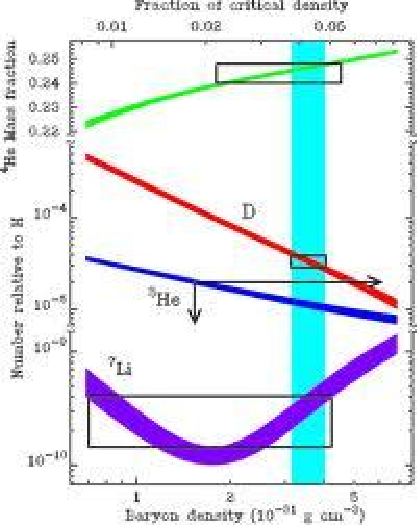
\includegraphics[width=0.5\textwidth]{figure/Abundances.pdf}
  \caption{Abbondanza vs $\rho_B(t_0)$}
  \label{fig:abbondanza}
\end{figure}

\section{Teoria dell'inflazione}
\label{sec:inflazione}

\emph{Queste note sono basate sulle lezioni di Inflazione tenute da Danièle
  Steer (APC Paris) durante l'IDPASC School 2015.}

\subsection{Problemi del modello standard della cosmologia}
\label{sec:problemi-cosmologia}

Il modello dell'Hot Big Bang è perfettamente soddisfacente per tempi \(t\gtrsim
\SI{e-3}{\second}\) dopo la singolarità iniziale, quindi prima della
nucleosintesi del Big Bang.  Questo modello è compatibile con la legge di Hubble
e descrive bene la nucleosintesi, la presenza di una radiazione di fondo a
microonde e la formazione e crescita delle struttura a larga scala.

Tuttavia, il modello è incompleto dal momento che le condizioni iniziali devono
essere fissate a mano.  Inoltre, ci sono alcuni problemi tuttora irrisolti, fra
i quali:
\begin{itemize}
\item l'origine e la natura della materia e dell'energia oscura,
\item il \emph{problema dei monopoli magnetici},
\item il \emph{problema della piattezza},
\item il \emph{problema dell'orizzonte}.
\end{itemize}
La teoria dell'\emph{inflazione}, sviluppata a partire dagli anni '70 del secolo
scorso soprattutto da parte di Guth e Linde, afferma che pochi istanti dopo il
Big Bang c'è stata una breve fase di rapida espansione accelerata dell'Universo,
quindi caratterizzata da \(\ddot{R}>0\).  La fase di inflazione sarebbe iniziata
circa \SI{e-36}{\second} dopo il Big Bang e sarebbe terminata fra circa
\SI{e-34}{\second} e \SI{e-32}{\second} dopo la singolarità iniziale.  Questo
fenomeno, se fosse avvenuto realmente, risolverebbe in un colpo solo tutti gli
ultimi tre problemi elencati.

La teoria dell'inflazione è un'aggiunta al modello standard della cosmologia,
non una nuova teoria alternativa a quella finora illustrata che rimane per il
resto inalterata.  A oggi non sono ancora state trovate evidenze sperimentali
che dimostrino la validità dell'inflazione, anche se ci sono forti motivazioni
teoriche che la fanno apparire ben fondata.

Nei seguenti paragrafi illustreremo i problemi dei monopoli magnetici, della
piattezza e dell'orizzonte, facendo inoltre vedere come la fase di inflazione li
risolverebbe.

\subsection{Problema dei monopoli magnetici}
\label{sec:problema-monopoli}

Secondo alcune teorie della grande unificazione, al termine della fase di
unificazione delle forze (\SI{e-36}{\second} dopo il Big Bang) si sarebbe
formato un gran numero di \emph{monopoli magnetici} (ipotetiche particelle
dotate di singola carica del campo magnetico) dotate di massa elevata.  Secondo
alcune stime~\parencite[143-145]{2002coec.book.....C}, i monopoli magnetici
dovrebbero avere massa \(m_{\textup{M}} \approx \SI{e16}{\giga\electronvolt}\) e
densità numerica attuale, escludendo che ci sia stata una fase di inflazione,
almeno dello stesso ordine di quella dei barioni.  Questo è chiaramente
incompatibile con le osservazioni attuali perché i monopoli magnetici non sono
mai stati trovati ma, soprattutto, la loro elevata massa combinata con la loro
densità numerica significherebbe che la densità di materia oggi dovrebbe essere
\(16\) ordini di grandezza più grande di quella misurata.

La fase di inflazione risolverebbe questo problema perché l'espansione
accelerata si collocherebbe dopo la formazione dei monopoli magnetici ma prima
della creazione della materia ordinaria che costituisce l'Universo che
conosciamo.  Pertanto, la rapida espansione porterebbe a una forte diminuzione
della densità dei soli monopoli magnetici, senza alterare la densità della
materia barionica.  Per fissare le idee, anticipiamo che il fattore di scala fra
l'inizio e la fine della fase di inflazione sarebbe aumentato di circa \num{e26}
volte, quindi la densità di monopoli sarebbe diminuita di un fattore dell'ordine
di \num{e78}.

\subsection{Problema della piattezza}
\label{sec:problema-piattezza}

Richiamiamo l'equazione di Friedmann~\eqref{eq:friedmann} nella forma
\begin{equation}
  \label{eq:friedmann2}
  H^{2}(t) = \left(\frac{\dot{R}(t)}{R(t)}\right)^{2} = \frac{8\pi G}{3}\rho(t)
  - \frac{k}{R^{2}(t)}.
\end{equation}
Con il parametro di densità \(\Omega(t) = \rho(t)/\rho_{\textup{c}}(t)\) si può
riscrivere come
\begin{equation}
  \label{eq:friedmann-densita}
  \Omega(t) - 1 = \frac{k}{R^{2}(t)H^{2}(t)}.
\end{equation}
Secondo gli ultimi dati del telescopio Planck~\parencite{2015arXiv150201589P},
oggi risulta \(\abs{\Omega(t_{0}) - 1} = \num{0.000(5)}\), cioè
\(\abs{\Omega(t_{0}) - 1} < \num{0.005}\).  Questo significa che oggi l'Universo
appare pressoché piatto.  Dall'analisi
dell'equazione~\eqref{eq:friedmann-densita} possiamo dedurre che
\begin{itemize}
\item o la costante \(k\) è nulla e quindi \(\Omega(t) - 1\) è sempre stata
  uguale a \(0\),
\item oppure \(\abs{\Omega(t) - 1}\) si evolve nel tempo come \((R(t)H(t))^{-2}
  = \dot{R}^{-2}(t)\).
\end{itemize}

Prima di procedere, ricordiamo che dall'equazione di
continuità~\eqref{eq:continuita} \(\dot{\rho} + 3H(p + \rho) = 0\) si ricava che
\begin{equation}
  \rho(R) \sim R^{-3(1+w)}
\end{equation}
con \(w = p/\rho\).  Poiché stiamo considerando un Universo approssimativamente
piatto, poniamo per semplicità \(k=0\) nell'equazione~\eqref{eq:friedmann2} e
inserendo il risultato precedente si ha
\begin{equation}
  \begin{split}
    H^{2} = \left(\frac{\dot{R}}{R}\right)^{2} \sim \rho = R^{-3(1+w)} &\implies
    \frac{1}{R} \toder{R}{t} \sim R^{-3(1+w)/2} \\
    &\implies R^{(3w+1)/2}\dd R \sim \dd t.
  \end{split}
\end{equation}
La soluzione di questa equazione differenziale dipende dal valore di \(w\).  Se
\(w\neq -1\) allora si trova che
\begin{equation}
  R(t) \sim t^{2/3(w+1)} = t^{\beta}
\end{equation}
con
\begin{equation}
  \beta = \frac{2}{3(w+1)} =
  \begin{cases}
    2/3 & \text{per la materia (\(w = 0\))}, \\
    1/2 & \text{per la radiazione (\(w = 1/3\))}.
  \end{cases}
\end{equation}
Invece se \(w = -1\) si ha che
\begin{equation}
  R(t) \sim \e^{Ht}.
\end{equation}
Ricapitolando abbiamo determinato
\begin{equation}
  R(t) \sim
  \begin{cases}
    t^{\beta} & \text{se \(w\neq -1\)}, \\
    \e^{Ht}  & \text{se \(w = -1\)}.
  \end{cases}
\end{equation}

\begin{figure}
  \centering
  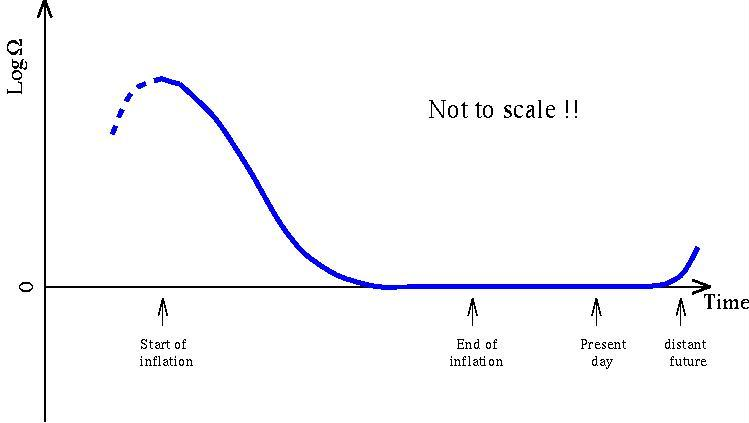
\includegraphics[width=\textwidth]{figure/flatness}
  \caption[Come l'inflazione risolve il problema della piattezza]{La teoria
    dell'inflazione risolve il problema della piattezza introducendo una fase in
    cui \(\abs{\Omega(t) - 1}\), rappresentata sull'asse delle ordinate, tende
    rapidamente verso \(0\), partendo da una condizione iniziale qualsiasi.  Al
    termine della fase di inflazione, \(\abs{\Omega(t) - 1}\) ha ripreso
    lentamente ad aumentare fino a raggiungere il valore attuale.  Immagine
    tratta da \url{https://ned.ipac.caltech.edu/level5/Liddle/Liddle4_1.html}}
  \label{fig:piattezza}
\end{figure}
Ora possiamo calcolare l'evoluzione di \(\abs{\Omega(t) - 1}\) con il tempo.
Supponiamo che l'Universo sia stato dominato solo dalla radiazione e dalla
materia, quindi possiamo assumere che risulti sempre \(\beta < 1\).  In questo
modo vediamo che
\begin{equation}
  \label{eq:omega-t}
  \abs{\Omega(t) - 1} \sim \dot{R}^{-2}(t) \sim \frac{t^{2(1-\beta)}}{\beta^{2}}
\end{equation}
è una funzione crescente col tempo.  Dunque, oggi l'Universo ha una densità
prossima alla densità critica, ma per quanto abbiamo trovato in passato la
densità era ancora più vicina alla densità critica.  Possiamo stimare quanto è
aumentato \(\abs{\Omega(t) - 1}\) fra il tempo di Planck \(t = t_{\textup{Pl}}
\sim \SI{e-43}{\second}\) e oggi (\(t = t_{0} \sim \SI{e17}{\second}\)).  Per
fare questo supponiamo un Universo sempre dominato dalla radiazione, quindi vale
sempre \(\beta = 1/2 \implies \abs{\Omega(t) - 1} \sim t\), da cui
\begin{equation}
  \frac{\abs{\Omega(t_{0}) - 1}}{\abs{\Omega(t_{\textup{Pl}}) - 1}} \sim
  \frac{10^{17}}{10^{-43}} = 10^{60}.
\end{equation}
Inoltre abbiamo visto che oggi si ha \(\abs{\Omega(t_{0}) - 1} \lesssim
10^{-3}\), quindi
\begin{equation}
  \abs{\Omega(t_{\textup{Pl}}) - 1} \lesssim 10^{-63}.
\end{equation}
Con questi approssimativi calcoli abbiamo trovato che subito dopo il Big Bang la
densità dell'Universo doveva differire dalla densità critica al più per una
parte su \(10^{-63}\).  Il modello standard della cosmologia non prevede che
l'Universo dovesse essere all'inizio praticamente piatto o quasi, bisogna
imporlo come condizione iniziale.  Questo non è un vero e proprio problema di
per sé, ma è un difetto nella teoria del modello standard perché comporta
fissare forzatamente la densità iniziale dell'Universo a un valore molto
particolare, quando non ci sono motivi per ritenere che questo valore fosse più
probabile di qualsiasi altro.  Si usa dire che questo è un problema di
\emph{fine-tuning}.

Il problema della piattezza sarebbe risolto se ci fosse stata una fase, nel
passato, in cui \(\abs{\Omega(t) - 1}\) fosse rapidamente sceso verso \(0\).
Questa è proprio la fase di inflazione.  Dall'equazione~\eqref{eq:omega-t} si
vede che questo è possibile se risulta \(\beta > 1\).  In questo caso
\(\abs{\Omega(t) - 1} \to 0\) è un attrattore per l'evoluzione del sistema,
qualunque sia stato il valore iniziale.  L'inflazione risolve dinamicamente il
problema del \emph{fine-tuning}: la densità iniziale dell'Universo aveva
effettivamente un valore qualsiasi, solo successivamente si è evoluta verso la
densità critica, per poi allontanarsi lentamente da essa al termine della fase
di inflazione, come mostrato nella figura~\ref{fig:piattezza}.

Osserviamo che se \(\beta>1\) risulta \(\ddot{R} = \beta(\beta-1)t^{\beta-2}
\implies \ddot{R} > 0\), cioè espansione accelerata dell'Universo, proprio come
prescritto dalla teoria dell'inflazione.  D'altra parte \(\beta = 2/3(w+1)>1\)
equivale a \(-1 < w < -1/3\) e dall'equazione di accelerazione
\(\ddot{R}/R=-4\pi G(\rho+3p)/3\) si ha che si ha espansione accelerata solo se
\(w < -1/3\).

\subsection{Problema dell'orizzonte}
\label{sec:problema-orizzonte}

L'origine di questo problema è la \emph{causalità}: la velocità della luce nel
vuoto fissa un limite superiore alla velocità di propagazione di qualsiasi
segnale.  Le mappe della radiazione cosmica di fondo realizzate dai telescopi
WMAP e Planck hanno mostrato che l'intero cielo a noi oggi visibile ha la stessa
temperatura, a meno di anisotropie dell'ordine di \(10^{-5}\), quindi
trascurabili in prima analisi.  È possibile che tutti i punti di una così vasta
regione dello spazio fossero in connessione causale al momento del
disaccoppiamento, in modo tale da giustificare un processo di termalizzazione
che abbia coinvolto tutto l'Universo visibile?

Definiamo \emph{orizzonte} \(d_{\textup{H}}(t,t_{i})\) come la massima distanza
percorsa da un raggio di luce emesso al tempo \(t_{i}\) e osservato al tempo
\(t\).  Questa quantità determina la distanza massima che ci può essere fra due
punti che sono in connessione causale l'uno con l'altro.  Matematicamente
abbiamo
\begin{equation}
  d_{\textup{H}}(t, t_{i}) = R(t)\int_{t_{i}}^{t} \frac{\dd t'}{R(t')} =
  \frac{R(t)}{1-\beta}(t^{1-\beta} - t_{i}^{1-\beta})
\end{equation}
avendo usato \(R(t)\sim t^{\beta}\).  Vogliamo determinare cosa succede provando
a considerare un segnale partito molto indietro nel tempo, diciamo per \(t_{i}
\to 0\).  Ci sono due possibilità:
\begin{itemize}
\item \(d_{\textup{H}}(t, t_{i})\) converge a un valore finito per \(t_{i} \to
  0\) e in questo caso il segnale emesso non può essere visto più lontano della
  distanza \(d_{\textup{H}}(t, t_{i})\),
\item oppure l'integrale diverge a un valore infinito, quindi è possibile
  ricevere segnali emessi a tempi sufficientemente remoti da qualsiasi sorgente
  comovente.
\end{itemize}
In un Universo sempre dominato solo da radiazione e materia risulta \(\beta<1\)
e quindi
\begin{equation}
  d_{\textup{H}}(t, t_{i}) \xrightarrow[t_{i}\to 0]{} \frac{R(t)
    t^{1-\beta}}{1-\beta} = \frac{\beta}{1-\beta} \frac{1}{H(t)}
\end{equation}
A parte il fattore numerico legato al valore di \(\beta\), la dimensione
dell'orizzonte è essenzialmente data dal raggio di Hubble \(1/H(t)\) e ci
troviamo nella prima delle due situazioni illustrate sopra.  Secondo questo
modello, col passare del tempo aumentano le frazioni dell'Universo che sono in
connessione causale.  Quindi esistono nella radiazione cosmica di fondo delle
regioni che erano disconnesse causalmente.  Ma a questo punto sorge il problema:
come è possibile spiegare l'omogeneità delle condizioni iniziali al momento
dell'ultimo scattering, quando è iniziata la radiazione cosmica di fondo?
Ancora una volta l'inflazione risolve il problema introducendo una fase con
\(\beta>1\), che abbiamo visto implicare espansione accelerata \(\ddot{R}>0\).
In questo caso si ha
\begin{equation}
  d_{\textup{H}}(t, t_{i}) \xrightarrow[t_{i}\to 0]{} \infty
\end{equation}
e sarebbe quindi stato possibile, per tutti i punti della radiazione che
osserviamo oggi, essere in connessione causale l'uno con l'altro.

\begin{figure}
  \centering
  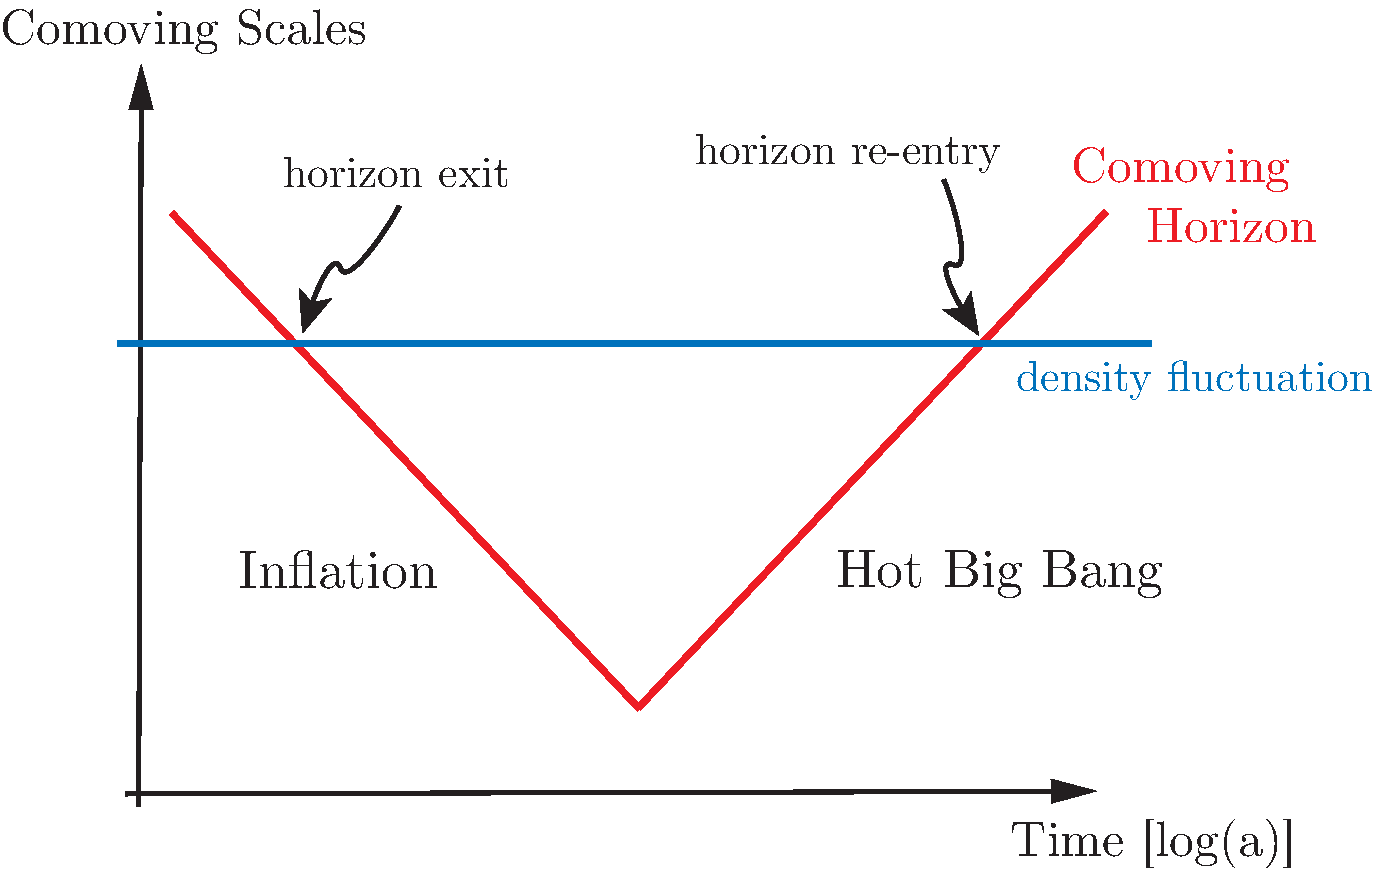
\includegraphics[width=0.55\textwidth]{figure/scales}\hfill
  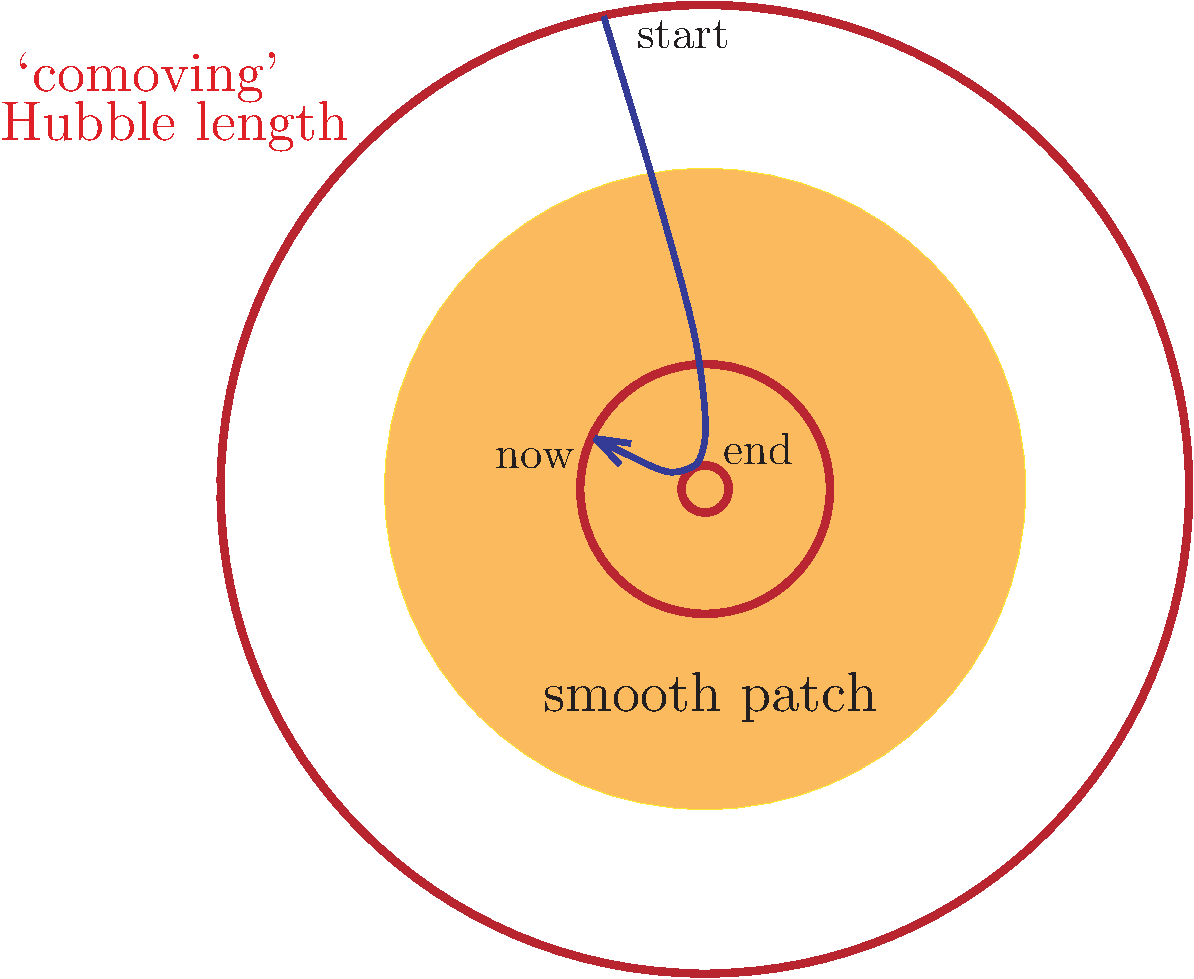
\includegraphics[width=0.4\textwidth]{figure/horizon}
  \caption[Come l'inflazione risolve il problema
  dell'orizzonte]{\emph{Sinistra}: andamento schematico del raggio comovente di
    Hubble \((RH)^{-1}\) con il tempo.  Durante l'inflazione è diminuito, per
    poi crescere nelle epoche della radiazione e della materia, previste dal
    modello dell'Hot Big Bang.  I punti che si trovano a una distanza pari al
    raggio comovente di Hubble attuale oggi sono in contatto causale, ma secondo
    quest'ultimo modello non possono mai esserlo stato nel passato.  Invece, se
    c'è stata una fase di inflazione le distanze dell'ordine di \((RH)^{-1}\)
    attuale sono state al di sotto dell'orizzonte in tempi sufficientemente
    remoti.  \emph{Destra}: evoluzione del raggio comovente di Hubble.  La sfera
    comovente di Hubble si è ristretta durante l'inflazione e allargata in
    seguito.  Figure tratte da~\cite[27]{2009arXiv0907.5424B}}
  \label{fig:orizzonte}
\end{figure}
Proviamo a illustrare un altro argomento che presenta il problema
dell'orizzonte.  Già nel problema della piattezza abbiamo incontrato
l'importante quantità
\begin{equation}
  \frac{1}{R(t)H(t)}
\end{equation}
chiamata \emph{raggio} o \emph{parametro di Hubble comovente}.  Il nome deriva
dal fatto che \(c/H(t) = 1/H(t)\) è il \emph{raggio di Hubble}, che indica la
tipica lunghezza di scala alla quale un processo fisico nell'Universo opera
coerentemente.  Dividendo per il fattore di scala si ottiene la corrispondente
grandezza comovente, che tiene conto della variazione di \(R(t)\).  Vediamo come
si evolve il parametro di Hubble comovente con il tempo.  Per parametrizzare il
tempo usiamo il fattore di scala, che sappiamo avere andamento \(R(t)\sim
t^{\beta}\), se \(w\neq -1\).  Nel caso dell'Universo dominato dalla radiazione
\(\beta = 1/2\), quindi
\begin{equation}
  \ln \frac{1}{RH} = \ln \frac{1}{\dot{R}} \sim \ln t^{1/2} \sim \ln R.
\end{equation}
Invece, nella fase dell'Universo dominato dalla materia abbiamo \(\beta = 2/3\),
da cui
\begin{equation}
  \ln \frac{1}{RH} = \ln \frac{1}{\dot{R}} \sim \ln t^{1/3} \sim \ln R^{1/2} =
  \frac{1}{2}\ln R.
\end{equation}
Quindi in ogni caso \(\ln (RH)^{-1}\) è una funzione crescente di \(\ln R\).  Ma
questo significa che regioni che oggi vediamo essere in contatto causale in
passato non potevano esserlo, dato che il raggio comovente di Hubble in passato
era molto più piccolo, quindi non c'è potuto essere un processo di
termalizzazione su una scala così grande.  Il problema si risolverebbe se in
passato, prima dell'inizio dell'epoca dominata dalla radiazione, c'è stata una
fase in cui \((RH)^{-1}\) è diminuito con il tempo, e quindi con \(R\).
Condizione necessaria affinché \((RH)^{-1}\) diminuisca con il tempo è che la
sua derivata temporale sia negativa, cioè
\begin{equation}
  0 > \toder{}{t} \frac{1}{RH} = \frac{1}{\dot{R}} =
  -\frac{\ddot{R}}{(\dot{R})^{2}} \iff \ddot{R}>0.
\end{equation}
Abbiamo di nuovo trovato che una fase inflazionaria di espansione accelerata
risolverebbe il problema dell'orizzonte: l'Universo prima dell'inflazione aveva
un raggio comovente di Hubble più grande di quello attuale, durante l'inflazione
il raggio è diminuito rapidamente, per poi ricominciare a crescere durante le
epoche della radiazione e della materia.  Le scale che noi oggi vediamo entrare
in connessione casuale lo erano già state in passato, prima dell'era della
radiazione, ed è in quel periodo che erano in corso i processi di
omogeneizzazione delle condizioni iniziali che hanno poi permesso alla
radiazione cosmica di fondo di avere una temperatura uniforme fra regioni che
credevamo non aver mai potuto comunicare fra di loro.  Per concretezza, durante
l'inflazione si assume che \(H\) sia rimasto costante, quindi
\begin{equation}
  \ln \frac{1}{RH} = \ln \frac{1}{R \cdot \text{costante}} \sim \ln \frac{1}{R}
  = - \ln R.
\end{equation}
Nella figura~\ref{fig:orizzonte} è rappresentato schematicamente l'andamento del
raggio comovente di Hubble secondo la teoria dell'inflazione.

\subsection{Quanta inflazione?}
\label{sec:quanta-inflazione}

Vogliamo determinare quanta inflazione c'è stata, cioè di quanto è aumentato il
fattore di scala durante la fase inflazionaria.  Calcoleremo questa quantità
prendendo spunto dal problema della piattezza.

Nella teoria dell'inflazione si quantifica l'espansione con il logaritmo del
rapporto fra il fattore di scala alla fine dell'inflazione (\(t_{f}\)) e
all'inizio (\(t_{i}\))
\begin{equation}
  N_{*} = \ln \frac{R(t_{f})}{R(t_{i})}.
\end{equation}
Questa quantità è chiamata \emph{numero di \(\e\)-foldings}, perché indica
quante \(\e = 2.718\dots\) volte si è espanso l'Universo in quella fase.

Assumiamo, senza perdita di generalità, che \(\abs{\Omega(t) - 1}\) all'inizio
dell'inflazione fosse dell'ordine dell'unità,\footnote{L'importante è che sia
  sostanzialmente diversa da \(0\).} quindi \(\abs{\Omega(t_{i}) - 1} \sim 1\).
Oggi sappiamo che risulta al più \(\abs{\Omega(t_{0}) - 1} \sim 0.001\), per
determinare \(\abs{\Omega(t_{f}) - 1}\) sfruttiamo \(\abs{\Omega(t) -1} \sim
t^{2(1-\beta)}\) e andiamo a ritroso nel tempo.  Ricordiamo che
\begin{itemize}
\item l'era della radiazione (\(\beta = 1/2\)) è iniziata al termine
  dell'inflazione (\(t \sim \SI{e-34}{\second}\)) ed è finita a \(t =
  \SI{4.7e4}{y} = \SI{1.5e12}{\second}\);
\item l'era della materia (\(\beta = 2/3\)) è iniziata al termine dell'era della
  radiazione ed è continuata quasi fino ai giorni nostri\footnote{Trascuriamo
    l'era dell'energia oscura, ininfluente ai fini di questi calcoli.} \(t =
  \SI{13.8e9}{y} = \SI{4.4e17}{\second}\).
\end{itemize}
Quindi risulta
\begin{equation}
  \abs{\Omega(t_{f}) - 1} = \abs{\Omega(t_{f}) - 1}
  \left(\frac{\num{4.4e17}}{\num{1.5e12}}\right)^{2(2/3-1)}
  \left(\frac{\num{1.5e12}}{\num{e-34}}\right)^{2(1/2-1)} = \num{1.5e-53}.
\end{equation}
Durante l'inflazione si assume \(H(t) = \text{costante}\), quindi in questa fase
\(\abs{\Omega(t_{f}) - 1} \sim R^{-2}\) e
\begin{equation}
  \frac{R(t_{f})}{R(t_{i})} = \sqrt{\frac{\abs{\Omega(t_{i}) -
        1}}{\abs{\Omega(t_{f}) - 1}}} = \num{2.6e26},
\end{equation}
da cui troviamo infine
\begin{equation}
  N_{*} = \ln \frac{R(t_{f})}{R(t_{i})} \approx 61.
\end{equation}
Dunque, usando come punto di partenza il problema dell'orizzonte, abbiamo
trovato che durante la breve fase di inflazione il fattore di scale è aumentato
di un fattore dell'ordine di \(10^{26}\), corrisponde a un numero di e-foldings
pari a circa \(60\).

\subsection{Inflazione vs energia oscura}
\label{sec:inflazione-energia-oscura}

Sia la fase di inflazione sia l'era dominata dall'energia oscura nella quale ci
troviamo oggi sono caratterizzate dall'espansione accelerata dell'Universo,
\(\ddot{R} > 0\), ma ci sono due differenze sostanziali fra queste due
situazioni
\begin{itemize}
\item le energie in gioco sono completamente differenti, infatti si calcola che
  il potenziale associato all'inflazione è dell'ordine di (\(M_{\textup{Pl}} =
  1/\sqrt{8\pi G}\) è la massa di Planck)
  \begin{equation}
    V_{\textup{inflazione}} \sim (M_{\textup{Pl}})^{4}
  \end{equation}
  mentre per l'energia oscura si trova
  \begin{equation}
    V_{\textup{energia oscura}} \sim (10^{-30}M_{\textup{Pl}})^{4}.
  \end{equation}
  Questo giustifica anche il fatto che il fattore di scala durante l'inflazione
  è aumentato in maniera molto più rapida rispetto all'aumento in corso oggi;
\item la fase di inflazione si è dovuta arrestare a un certo punto della storia
  dell'Universo, per dare spazio alle ere di dominio della radiazione e della
  materia, mentre non conosciamo ancora il destino dell'espansione attuale
  guidata dall'energia oscura, che in base alle nostre conoscenze potrebbe anche
  durare per sempre.
\end{itemize}

\subsection{Regime di slow-roll e potenziale di inflazione}
\label{sec:slow-roll}

La costante cosmologica è un esempio di modello per descrivere un Universo in
espansione accelerata, ma abbiamo ricordato che l'inflazione deve avere
necessariamente avuto una fine.  Affinché questo sia avvenuto, c'è bisogno di
introdurre una dipendenza dal tempo nel modello dell'inflazione e si fa questo
introduce un campo scalare inflatonico \(\phi\) che guida l'evoluzione
dell'Universo in questa fase, con un potenziale associato \(V(\phi)\) che evolve
nel tempo.  In questo paragrafo vedremo sotto quali condizioni si verifica la
fase di inflazione.

Per descrivere l'inflazione si aggiunge all'azione del campo gravitazionale
l'azione associata al campo inflatonico \(\phi\) data da
\begin{equation}
  S_{\phi} = \int\dd^{4}x
  \sqrt{-g}\left(-\frac{1}{2}(\partial_{\mu}\phi)(\partial^{\mu}\phi) -
    V(\phi)\right)
\end{equation}
da cui si ricava il tensore di energia-impulso
\begin{equation}
  T_{\mu\nu} = \frac{2}{\sqrt{-g}} \frac{\delta S_{\phi}}{\delta g_{\mu\nu}}
  = \partial_{\mu}\phi \partial_{\nu}\phi -
  g_{\mu\nu}\left(\frac{1}{2}\partial_{\sigma}\phi \partial^{\sigma}\phi -
    V\right)
\end{equation}
e l'equazione del moto
\begin{equation}
  \nabla_{\mu}\nabla^{\mu}\phi = \toder{V}{\phi}.
\end{equation}
Inoltre si possono calcolare la pressione e la densità del campo inflatonico
\begin{align}
  \rho &= -\tensor{T}{^{0}_{0}} = \frac{1}{2}\dot{\phi}^{2} + V, \\
  p &= \frac{1}{2}\dot{\phi}^{2} - V.
\end{align}
L'equazione del moto si può riscrivere come
\begin{equation}
  \ddot{\phi} + 3H\dot{\phi} + V' = 0,
\end{equation}
in cui \(V' = \ltoder{V}{\phi}\).  L'equazione di stato stato del campo
inflatonico è
\begin{equation}
  w = \frac{p}{\rho} = \frac{\dot{\phi}^{2}/2 - V}{\dot{\phi}^{2}/2 + V}.
\end{equation}
Risulta \(-1<w<1\), con \(-1\) corrispondente al caso limite \(\dot{\phi}^{2}/2
\ll V\) e \(1\) al caso \(\dot{\phi}^{2}/2 \gg V\).  L'inflazione richiede che
ci sia espansione accelerata e come abbiamo già visto questo corrisponde alla
condizione \(w < -1/3\), quindi l'energia cinetica del campo è molto più piccola
del potenziale.  Questo porta alla definizione del \emph{regime di slow-roll},
durante il quale, secondo le moderne teorie dell'inflazione, è avvenuta
l'espansione accelerata primordiale.  Lo slow-roll è caratterizzato da due
condizioni
\begin{itemize}
\item energia cinetica del campo inflatonico molto più piccola del suo
  potenziale, \(\dot{\phi}^{2}/2 \ll V\);
\item accelerazione del campo trascurabile nell'equazione del moto,
  \(\abs{\ddot{\phi}}\ll \abs{3H\dot{\phi}}\), \(\abs{V'}\).
\end{itemize}
Dalla prima condizione abbiamo che l'equazione di Friedmann si può scrivere come
\begin{equation}
  H^{2} = \frac{8\pi G}{3}\rho \approx \frac{8\pi G}{3}V
\end{equation}
e dalla seconda condizione l'equazione del moto diventa
\begin{equation}
  3H\dot{\phi} + V' = 0.
\end{equation}
Inoltre risulta \(w \approx -1\), quindi durante l'inflazione il fattore di
scala va come \(R(t)\sim \e^{Ht}\).

Nelle teorie d'inflazione si introducono due parametri
\begin{align}
  \epsilon_{V} &\equiv
  \frac{M_{\textup{Pl}}^{2}}{2}\left(\frac{V'}{V}\right)^{2}, \\
  \eta_{V} &\equiv M_{\textup{Pl}}^{2}\frac{V''}{V}.
\end{align}
Usando entrambe le condizioni che determinano il regime di slow-roll si vede che
affinché si abbia l'inflazione deve risultare
\begin{align}
  \epsilon_{V} &\ll 1, \\
  \abs{\eta_{V}} &\ll 1.
\end{align}
La fase di inflazione termina quando le condizioni di slow-roll non sono più
soddisfatte.  In particolare, calcolando \(\dot{H} = \ddot{R}/R - H^{2}\) si può
ricavare che \(\ddot{R}/R = H^{2}(1 - \epsilon_{V})\), quindi l'inflazione ha
avuto fine quando si è raggiunta la condizione
\begin{equation}
  \ddot{R} = 0 \implies \epsilon_{V} = 1.
\end{equation}

Esistono diversi modelli di inflazione: tutti prevedono una breve fase di rapida
espansione accelerata, ma cambiano i parametri del sistema, come il numero di
e-foldings, e l'espressione del potenziale inflatonico.  Riportiamo che in base
alle ultime analisi fatte dalla collaborazione di
Planck~\parencite{2015arXiv150202114P} il potenziale che risulta favorito è il
\emph{potenziale di Starobinsky}
\begin{equation}
  V(\phi) \propto (1 - \e^{\sqrt{2/3}\phi/M_{\textup{Pl}}})^{2}
\end{equation}
e con \(N_{*} = 60\).  Questo modello è anche chiamato \emph{inflazione
  \(R^{2}\)} perché si modifica l'azione del campo gravitazionale aggiungendo un
termine quadratico nella curvatura scalare \(S \sim \int\dd^{4}x\sqrt{-g}(R +
R^{2})\).

%%% Local Variables:
%%% mode: latex
%%% TeX-master: "../cosmo"
%%% fill-column: 80
%%% End:


\backmatter{}

\cleardoublepage{}
\phantomsection
\addcontentsline{toc}{chapter}{\refname}
\printbibliography

% \cleardoublepage{}
% \phantomsection
% \addcontentsline{toc}{chapter}{\indexname}
% \printindex{}

\end{document}

%%% Local Variables:
%%% mode: latex
%%% TeX-master: t
%%% fill-column: 80
%%% End:
